\documentclass[10pt]{book}
\usepackage[fontsize=9pt]{scrextend}

\setcounter{section}{0}
\setlength\parindent{10pt}

\usepackage[b5paper,
    inner=16mm,         % Inner margin
    outer=24mm,         % Outer margin
    bindingoffset=10mm, % Binding offset
    top=28mm,           % Top margin
    bottom=28mm,        % Bottom margin
]{geometry}
\usepackage[utf8]{inputenc}
\usepackage{amsmath, amsthm, amsfonts, kotex, enumitem, setspace, lipsum, amssymb, tabularray, mathtools, chngcntr, tikz, tikz-cd, graphicx, scalerel, graphbox, stmaryrd, float, colortbl, multirow, multicol, caption, subcaption, pgffor, appendix, makeidx, physics, gensymb, footnote, cancel}
\usepackage[colorlinks=true,linkcolor=blue,citecolor=blue]{hyperref}
% \let\Bbbk\relax
% \usepackage{newtxtext, newtxmath}
\usepackage{libertineRoman, libertineMono}
\usepackage[T1]{fontenc}
\usepackage[notextcomp]{stix}
\setstretch{1.4}
\usepackage[symbol]{footmisc}
% \usepackage[bottom]{footmisc}
% \usepackage{microtype}
% \usepackage{silence}

% % Ignore all warnings about font size substitutions
% \WarningFilter{font}{Font shape `T1/cmss/m/n' in size}

\usepackage{iftex}
\ifPDFTeX
    \usepackage{dhucs-nanumfont}
    % \usepackage{newtxmath}
\else\ifXeTeX
      \usepackage{fontspec}
      \setmainhangulfont{NanumMyeongjo}[%
    	Renderer = OpenType,
    	FontFace = {m}{n}{ Font = * },
    	FontFace = {m}{it}{ Font = *, FakeSlant=.167 },
    	FontFace = {m}{up}{ Font = * },
    	FontFace = {bx}{n}{ Font = {* ExtraBold} },
    	FontFace = {bx}{it}{ Font = {* ExtraBold}, FakeSlant=.167 }
    ]
    \setsanshangulfont{NanumGothic}
\else\ifLuaTeX
  \usepackage{fontspec}
      \setmainfont{Times New Roman}
      \setmainhangulfont{NanumMyeongjo}[%
    	Renderer = OpenType,
    	FontFace = {m}{n}{ Font = * },
    	FontFace = {m}{it}{ Font = *, FakeSlant=.167 },
    	FontFace = {m}{up}{ Font = * },
    	FontFace = {bx}{n}{ Font = {* ExtraBold} },
    	FontFace = {bx}{it}{ Font = {* ExtraBold}, FakeSlant=.167 }
    ]
    \setsanshangulfont{NanumGothic}
\fi\fi\fi


% Upper cases

\foreach \x in {A,...,Z}{%
\expandafter\xdef\csname bb\x\endcsname{\noexpand\ensuremath{\noexpand\mathbb{\x}}}
\expandafter\xdef\csname cal\x\endcsname{\noexpand\ensuremath{\noexpand\mathcal{\x}}}
\expandafter\xdef\csname frak\x\endcsname{\noexpand\ensuremath{\noexpand\mathfrak{\x}}}
\expandafter\xdef\csname bf\x\endcsname{\noexpand\ensuremath{\noexpand\mathbf{\x}}}
}

\newcommand{\NN}{\bbN}
\newcommand{\ZZ}{\bbZ}
\newcommand{\QQ}{\bbQ}
\newcommand{\RR}{\bbR}
\newcommand{\CC}{\bbC}
\newcommand{\FF}{\bbF}

% Lower cases

\foreach \x in {a,...,z}{%
\expandafter\xdef\csname frak\x\endcsname{\noexpand\ensuremath{\noexpand\mathfrak{\x}}}
\expandafter\xdef\csname bf\x\endcsname{\noexpand\ensuremath{\noexpand\mathbf{\x}}}
}


% Brackets

\newcommand{\inner}[2]{\left\langle#1, #2\right\rangle}

\newcommand{\gen}[1]{\left\langle#1\right\rangle}

\newcommand{\floor}[1]{\left\lfloor#1\right\rfloor}
\newcommand{\ceil}[1]{\left\lceil#1\right\rceil}

% Operators

\DeclareMathOperator{\difform}{d\!}

% Shortcuts

\newcommand{\vn}{\varnothing}

\newcommand{\eps}{\varepsilon}
\newcommand{\dt}{\delta}
\newcommand{\one}{\mathbf{1}}

\newcommand{\xR}{\RR^{\star}}

\newcommand{\seq}[2][\NN]{(#2_n)_{n \in #1}}
\newcommand{\subseq}[1]{(#1_{n(k)})_{k \in \NN}}
\newcommand{\sub}{\subseteq}
\newcommand{\pa}{\partial}
\newcommand{\setm}{\setminus}

\newcommand{\lop}{L'H\^opital}
\newcommand{\sch}{Schr\"odinger}

\newcommand{\toto}{\rightrightarrows}
\newcommand{\supnorm}[1]{\norm{#1}_{\sup}}

\newcommand{\longto}{\longrightarrow}


\newenvironment{enum}
	{\begin{enumerate}[leftmargin=*, noitemsep, topsep=2pt, label={\sf (\alph*)}]}
	{\end{enumerate}}

\newenvironment{enumroman}
	{\begin{enumerate}[leftmargin=*, noitemsep, topsep=2pt, label={\sf (\roman*)}]}
	{\end{enumerate}}

\numberwithin{equation}{section}

\usepackage{kotex}
\usepackage{amsthm, thmtools}
\usepackage{ hyperref,%\autoref % n.b. \Autoref is defined by thmtools
cleveref,% \cref % n.b. cleveref after! hyperref
}

\usepackage[framemethod=TikZ]{mdframed}
\mdfsetup{skipabove=2em,skipbelow=2em}

\theoremstyle{definition}
\declaretheoremstyle[
    headfont=\sffamily\bfseries, bodyfont=\normalfont,
    % mdframed={
    %     linewidth=2pt,
    %     rightline=true, topline=false, bottomline=false,
    %     linecolor=black, backgroundcolor=black!3!white,
    % }
]{thmbox}

\declaretheoremstyle[
    headfont=\sffamily\color{black!70!black}, bodyfont=\normalfont,
    numbered=no,
    % mdframed={
    %     linewidth=0pt,
    %     rightline=false, topline=false, bottomline=false,
    %     linecolor=black, backgroundcolor=black!2!white,
    % },
    qed=\qedsymbol
]{thmproofbox}

\theoremstyle{definition}
\declaretheoremstyle[
    headfont=\bfseries\sffamily\color{black!70!black}, bodyfont=\normalfont,
    % mdframed={
    %     linewidth=0pt,
    %     rightline=false, topline=false, bottomline=false,
    %     linecolor=black, backgroundcolor=black!3!white,
    % }
]{exerbox} 

\declaretheorem[numberwithin=section,style=thmbox, name=정의, refname={정의, 정의}, Refname={정의, 정의}]{defn}
\declaretheorem[sibling=defn,style=thmbox, name=예시, refname={예시,예시}, Refname={예시,예시}]{eg}
\declaretheorem[sibling=defn,style=thmbox, name=명제, refname={명제, 명제}, Refname={명제, 명제}]{prop}
\declaretheorem[sibling=defn,style=thmbox, name=정리, refname={정리, 정리}, Refname={정리, 정리}]{thm}
\declaretheorem[sibling=defn,style=thmbox, name=도움정리, refname={도움정리, 도움정리}, Refname={도움정리, 도움정리}]{lem}
\declaretheorem[sibling=defn,style=thmbox, name=따름정리, refname={따름정리, 따름정리}, Refname={따름정리, 따름정리}]{cor}
\declaretheorem[sibling=defn,style=thmbox, name=법칙, refname={법칙, 법칙}, Refname={법칙, 법칙}]{law}
\declaretheorem[sibling=defn,style=thmbox, name=관찰, refname={관찰, 관찰}, Refname={관찰, 관찰}]{obs}
\declaretheorem[sibling=defn,style=thmbox, name=주의, refname={주의, 주의}, Refname={주의, 주의}]{warn}
\declaretheorem[sibling=defn,style=thmbox, name=질문, refname={질문, 질문}, Refname={질문, 질문}]{que}
\declaretheorem[sibling=defn,style=thmbox, name=사실, refname={사실, 사실}, Refname={사실, 사실}]{fact}
\declaretheorem[sibling=defn,style=thmbox, name=논의, refname={논의, 논의}, Refname={논의, 논의}]{rem}
\declaretheorem[sibling=defn,style=thmbox, name=표기, refname={표기, 표기}, Refname={표기, 표기}]{notn}
\declaretheorem[sibling=defn,style=exerbox, name=연습문제, refname={연습문제, 연습문제}, Refname={연습문제, 연습문제}]{exr}
\declaretheorem[sibling=defn,style=exerbox, name=*연습문제, refname={*연습문제, *연습문제}, Refname={*연습문제, *연습문제}]{exrhard}

\declaretheorem[style=thmbox, name=주장, refname={주장, 주장}, Refname={주장, 주장}]{claim}
\declaretheorem[style=thmbox, numbered=no, name=주장, refname={주장, 주장}, Refname={주장, 주장}]{claimnonumbered}

\declaretheorem[style=thmbox, numbered=no, name=논의, refname={논의, 논의}, Refname={논의, 논의}]{remnonum}

\declaretheorem[style=thmproofbox, name=증명]{replacementproof}
\renewenvironment{proof}[1][]{\begin{replacementproof}[name=#1]}{\end{replacementproof}}

\usepackage[most]{tcolorbox}

\newenvironment{sketch}[1][\textbf{\textsf{[연습장]}}]
{\begin{tcolorbox}[boxrule=0.1mm, breakable]
\begin{center}
#1
\end{center}
}
{\end{tcolorbox}}


% \usepackage{tablefootnote} 
% \makeatletter 
% \AfterEndEnvironment{mdframed}{%
%  \tfn@tablefootnoteprintout% 
%  \gdef\tfn@fnt{0}% 
% }
% \makeatother 

\newcommand{\tablefootnote}{\footnote}

\allowdisplaybreaks
\usepackage{epigraph}
\usepackage{fancyhdr}
% \usepackage{fontspec}
\usepackage{emptypage}
\newcommand*{\blankpage}{
{\newpage \vspace*{5cm}\thispagestyle{empty}\centering \bfseries  \textit{This page is intentionally left blank.} \par}
\vspace{\fill}}
\let\uwu=\cleardoublepage

%titlepage
\renewcommand\epigraphflush{flushright}
\renewcommand\epigraphsize{\normalsize}
\setlength\epigraphwidth{0.7\textwidth}

\DeclareFixedFont{\titlefont}{T1}{ppl}{bx}{n}{0.75in}

\makeatletter                       
\def\printauthordate{%                  
    {\large \@author \\
    \smallskip
    \@date\\
    \bigskip
    정수출판사}}              
\makeatother
\author{한준영}
\date{\today}

\newcommand\titlepagedecoration{%
\begin{tikzpicture}[remember picture,overlay,shorten >= -10pt]

\coordinate (aux1) at ([yshift=-15pt]current page.north east);
\coordinate (aux2) at ([yshift=-410pt]current page.north east);
\coordinate (aux3) at ([xshift=-4.5cm]current page.north east);
\coordinate (aux4) at ([yshift=-150pt]current page.north east);

\begin{scope}[black!40,line width=12pt,rounded corners=12pt]
\draw
  (aux1) -- coordinate (a)
  ++(225:5) --
  ++(-45:5.1) coordinate (b);
\draw[shorten <= -10pt]
  (aux3) --
  (a) --
  (aux1);
\draw[opacity=0.6,black,shorten <= -10pt]
  (b) --
  ++(225:2.2) --
  ++(-45:2.2);
\end{scope}
\draw[black,line width=8pt,rounded corners=8pt,shorten <= -10pt]
  (aux4) --
  ++(225:0.8) --
  ++(-45:0.8);
\begin{scope}[black!70,line width=6pt,rounded corners=8pt]
\draw[shorten <= -10pt]
  (aux2) --
  ++(225:3) coordinate[pos=0.45] (c) --
  ++(-45:3.1);
\draw
  (aux2) --
  (c) --
  ++(135:2.5) --
  ++(45:2.5) --
  ++(-45:2.5) coordinate[pos=0.3] (d);   
\draw 
  (d) -- +(45:1);
\end{scope}
\end{tikzpicture}%
}

\usepackage{titlesec}% <-- to change chapter, section,... style
\usepackage[titles]{tocloft}% <-- changes to ToC
\cftsetindents{chapter}{0ex}{5ex}
\cftsetindents{section}{5ex}{6ex}
\cftsetindents{subsection}{11ex}{7ex}
    

\usepackage{titlesec}
\renewcommand{\chaptername}{장}
\titleformat{\chapter}[display]
  {\Huge\bfseries}{\thechapter~\chaptername}{20pt}{\Huge\bfseries}

\titleformat{\section}
{\normalfont\Large\bfseries}{~\thesection}{1em}{}
\newcommand{\sectionbreak}{\ifnum\value{section}>1 \clearpage\fi}


\usepackage{fancyhdr}
\renewcommand{\chaptermark}[1]{\markboth{\thechapter.~~#1}{}}
\renewcommand{\sectionmark}[1]{\markright{\thesection.~~#1}}
\pagestyle{fancy}
\fancyhf{}
\fancyhead[LO]{\rightmark}
\fancyhead[RE]{\leftmark}
\fancyhead[LE,RO]{\thepage}
\setlength{\headheight}{15pt}
\addtolength{\topmargin}{-2.5pt}



\begin{document}

\frontmatter
\pagestyle{empty}
\begin{titlepage}
    \vspace*{2cm}
    
    \noindent
    \vspace*{0.5cm}
    {\Huge \bf 물리화학의 정수 1}
    
    \vspace{1.5cm}
    \epigraph{{\it \large Essence of Undergraduate Physical Chemistry, Volume I}}%
    { \textsc{1st Edition}}
    \null\vfill
    \vspace*{1cm}
    \noindent
    \hfill
    \begin{minipage}{0.7\linewidth}
        \begin{flushright}
            \printauthordate
        \end{flushright}
    \end{minipage}
    %
    \begin{minipage}{0.02\linewidth}
        \rule{1pt}{70pt}
    \end{minipage}
    \titlepagedecoration
\end{titlepage}

\pagestyle{plain}
\chapter*{머리말}
\addcontentsline{toc}{chapter}{머리말}
    \section{감사의 말}
        \hspace{\parindent} 내용을 정리할 때 가장 큰 도움을 준 책 \textit{Atkins' Physical Chemistry}의 저자 Peter Atkins, Julio de Paula, 그리고 James Keeler 교수님들께 감사드립니다. 그리고 선대군 솔루션 제작방 인원들께 감사드립니다. 이 \textbf{정수} 시리즈는 여기에서 처음 시작되었으며, 최초로 쓰여진 \textbf{정수} 시리즈는 이진문\footnote[1]{서울대학교 자연과학대학 수리과학부 20학번}의 \cite{LeeEssTop}입니다. 이 책은 백인혁\footnote[2]{서울대학교 의과대학 의학과 20학번}의 해석개론의 정수\cite{BaekEssUGAna} 양식을 참고하였습니다. 그리고 다른 정수 시리즈는 홍승주\footnote[3]{서울대학교 자연과학대학 물리$\cdot$천문학부 학부 17학번, 석박통합 21학번}의 양자역학의 정수\cite{HongEssQPhys}가 있습니다. 이 분들과 선대군 솔루션 제작방의 다른 모든 분들께 감사드립니다.
    \section{들어가며}
        \hspace{\parindent} 이 문서는 물리화학의 기본 개념을 정리하고, 그 개념들이 어떻게 유도되는지 정리하기 위해 작성되었습니다.
        이 시리즈는 총 3개의 권으로 구성되며, 1권에서는 열역학을 정리합니다. Atkins' Physical Chemistry 11판을 기준으로,
        이 부분은 챕터 1부터 6까지에 해당합니다.
        \par 2권에서는 양자화학을 정리합니다. 이 부분은 챕터 7부터 11까지, 그리고 챕터 16에 해당합니다. 3권에서는 통계물리와 반응속도론,
        고체화학 및 표면화학에 이르는 넓은 범위를 정리합니다. 이 부분은 챕터 12부터 15까지, 그리고 챕터 17부터 19까지에 해당합니다.
        \par 본 책에서는 열역학에 대해 정리합니다. 먼저 1단원에서 기체에 대해 다루고, 2단원에서 열역학 제1 법칙을 다룹니다. 
        3단원에서는 열역학 제2 및 제3 법칙을 다루면서 단일 상황에 대한 열역학 과정을 다루게 됩니다.
        \par 이후 4단원 및 5단원에서는 상평형도에 대해 
        다룹니다. 구체적으로 4단원에서는 단일 물질의 상평형도를, 5단원에서는 혼합물의 상평형도를 다룹니다. 마지막으로 6단원에서는 화학 평형과 
        전기화학 기초를 다룹니다.
    \section{에너지에 관하여}
        \hspace{\parindent} 화학에서 에너지의 출입은 \textbf{열역학}의 언어로 기술된다. 이는 거시적인 물체에 적용되며, 3개의 법칙으로 기술된다. 
        단일 원자나 분자의 에너지에 대해서는 \textbf{양자역학}의 언어로 기술된다. 이에 대해서는 2권에서 더 자세히 다룰 예정이다. 
        입자의 운동에 관여하는 에너지는 양자화(Quantized) 되어 있으며, 병진 운동(Translation), 회전 운동(Rotation), 진동 운동(Vibration)의 
        세 가지 운동이 존재한다. 병진 운동 에너지의 준위 간 차이가 매우 작아($\sim 10^{-23}$ eV) 거의 연속적이다. 또한 
        회전 운동의 에너지 준위 간 차이는 약 0.001 eV, 진동 운동에서는 약 0.1 eV, 전자의 에너지 준위 간 차이는 수$\sim$수십 eV이다.
        \par 단일 입자의 에너지와 열역학 사이에는 \textbf{통계역학}이라는 다리가 존재한다. 입자의 분포 $N_i$와 에너지 $\varepsilon_{i}$, 
        절대온도 $T$ 사이에는 다음과 같은 관계가 성립한다:
        \begin{equation*}
            N_i \propto e^{- \frac{\varepsilon_{i}}{kT}}
        \end{equation*}
        이때 $k$는 \textit{Boltzmann 상수(Boltzmann's constant)}라 부르며, 그 값은 $1.380 \ 6488 \times 10^{-23}$ \textrm{J K$^{-1}$}에 해당한다. 이러한 
        분포를 \textit{Boltzmann 분포(Boltzmann distribution)}라 한다. 이에 대해서는 3권에서 더 자세히 다룰 예정이다.
\renewcommand{\contentsname}{차례}
\tableofcontents

\mainmatter
\pagestyle{fancy}

\chapter{기체의 성질}
        \section{이상 기체}
            \hspace{\parindent} 기체의 상태를 나타내는 변수에는 압력, 온도, 부피, 몰수가 있다. 각 변수에 대응되는 SI 단위는 \textrm{Pa(= N m$^{-2}$), K, m$^3$, mol}이다.
            \begin{defn}[표준 압력]
            $1$ \textrm{bar}(= $10^5$ \textrm{Pa})의 압력을 \textbf{표준 압력(Standard pressure)}이라 하고, 기호로 $p^{\circlehbar}$으로 나타낸다.
            \end{defn}
            $0$ \degree\textrm{C}는 273.15 \textrm{K}로 정의된다. 상태방정식은 일반적으로 다음과 같이 표현된다:
                \begin{defn}[상태방정식]
                    $p = f \left( T,V,n \right)$
                \end{defn}
            경험적인 법칙으로부터 다음과 같은 법칙들을 유도할 수 있다:
                \begin{obs}[Boyle의 법칙]
                    $pV = \text{일정, 단 }n \text{과 }T \text{가 일정}$
                \end{obs}
                \begin{obs}[Charles의 법칙(1)]
                    $V = \text{상수} \times T \text{, 단 }n \text{과 }p \text{가 일정}$
                \end{obs}
                \begin{obs}[Charles의 법칙(2)]
                    $p = \text{상수} \times T \text{, 단 }n \text{과 }V \text{가 일정}$
                \end{obs}
                \begin{obs}[Boyle-Charles 법칙]
                    $\displaystyle\frac{pV}{T} = \text{일정, 단 }n \text{이 일정}$
                \end{obs}
                \begin{obs}[Avogadro의 법칙]
                    $V = \text{상수} \times n \text{ , 단 }p \text{와 } T \text{가 일정}$
                \end{obs}
            같은 온도를 나타낸 곡선을 \textbf{등온 곡선(Isotherm)}, 같은 압력을 나타낸 곡선을 \textbf{등압 곡선(Isobar)}, 
            같은 부피를 나타낸 곡선을 \textbf{등적 곡선(Isochore)}이라고 한다.\\
            따라서 다음과 같은 \textbf{이상 기체 상태방정식}을 유도할 수 있다:
                \begin{thm}[이상 기체 상태방정식]
                    $pV = nRT$
                \end{thm}
            이때 $R$을 \textbf{기체 상수(Gas constant)}라 하고, 그 값은 $8.314\,4621$ \textrm{J K$^{-1}$ mol$^{-1}$}이다. 
            실제 기체는 $p \rightarrow 0$일 때 이상 기체와 유사하게 거동한다.
            \par 물질의 상태를 나타낼 때 온도와 압력을 표시해야 할 때가 많다. 대표적으로 다음과 같은 것들이 있다.
            \begin{defn}[SATP]
                $298.15$ \textrm{K}, $1$ \textrm{bar}를 Standard Ambient Temperature and Pressure, \textbf{SATP}라 한다.
            \end{defn}
            \begin{defn}[STP]
            $273.15$ \textrm{K}, $1$ \textrm{atm}를 Standard Temperature and Pressure, \textbf{STP}라 한다.
            \end{defn}
            STP에서 기체 $1$ \textrm{mol}의 부피는 
            $22.414$ \textrm{dm}$^3$에 해당한다.
            \begin{defn}[몰 부피]
            기체 1 \textrm{mol}의 부피를 $V_m$으로 나타내고, $V_m = V/n$을 만족한다.
            \end{defn}
            \par 혼합 기체에서는, 기체 각 성분의 \textbf{부분 압력(Partial pressure)}을 고려한다. 성분 $J$의 부분 압력 $p_J$는 다음과 같이 정의된다.
            \begin{defn}[부분 압력]
                $p_J = x_J p$
            \end{defn}
            이때 $x_J$는 성분 $J$의 \textbf{몰 분율(Mole fraction)}이고, 총 몰수 $n$에 대해 다음과 같이 정의된다.
                \begin{defn}[몰 분율]
                    $x_J = \displaystyle\frac{n_J}{n}, n = n_A + n_B + \cdots$
                \end{defn}
            $J$가 존재하지 않을 때에는 $x_J = 0$이고, $J$만 존재할 때에는 $x_J = 1$이다. 
            \begin{cor}
                모든 성분에 대해 $\displaystyle\sum_{J} x_J = 1$을 만족한다.
            \end{cor} 
            따라서 다음을 만족한다.
                \begin{cor}
                    $\displaystyle\sum_{J} p_J = \left( \sum_{J} x_J \right) p = p$
                \end{cor}
            이 관계는 이상 기체와 실제 기체 모두에서 적용된다. 이는 \textbf{Dalton 법칙(Dalton's law)}으로부터 유도된다.
            \begin{law}[Dalton 법칙]
            혼합 기체의 압력은 각 성분이 용기를 홀로 차지할 때 작용하는 압력의 합과 같다.
            \end{law}
            \begin{warn}
            \textbf{이 관계는 이상 기체에만 적용된다.} 그러나 \textbf{부분 압력은 모든 기체에 적용 가능하다.}
            \end{warn}
        \section{기체 분자 운동론}
            \hspace{\parindent} 기체 분자 운동론을 통해 이상 기체 상태방정식을 유도해 보자.
            \begin{rem}[기체 분자 운동론의 가정]
            기체 분자 운동론은 다음의 세 가지 가정으로부터 출발한다.
                \begin{enum}
                    \item 기체는 고전 역학을 따르는, 끊임없는 무작위 운동을 한다.
                    \item 분자의 크기는 무시 가능하다: 충돌과 충돌 간 기체 분자가 움직이는 거리보다 기체 분자 자체의 크기는 매우 작아서, 분자를 점으로 취급 가능하다.
                    \item 분자 간에는 완전 탄성 충돌만으로 상호작용한다.
                \end{enum}
            \end{rem}
            \begin{proof}
            운동량 보존에 의해, 분자는 충돌 전 $x$방향으로 $mv_x$의 운동량을 가지고, $x$축에 수직인 벽과 충돌 후에는 $-mv_x$의 운동량을 가진다. $\Delta t$의 
            시간 후에 이 분자가 벽과 충돌한다고 가정했을 때, 벽과의 거리가 $v_x \Delta t$ 이내이고 벽을 향해 운동하는 분자는 모두 벽과 충돌한다. 
            벽의 면적이 $A$라 할 때, 이 공간의 부피는 $Av_x \Delta t$이다.
            \par 입자의 몰수가 $n$, 용기의 부피가 $V$일 때 기체의 
            개수-밀도(number density)는 $\displaystyle\frac{n N_A}{V}$ ($N_A$는 아보가드로수)이므로, $Av_x \Delta t$의 부피 내에 있는 기체 분자 수는 
            $\displaystyle\frac{n N_A A v_x \Delta t}{V}$이다. 그러나 분자가 벽을 향해 운동할 확률은 $\displaystyle\frac{1}{2}$이고, 한편 운동량의 변화량은 $2mv_x$이므로, 
            운동량의 변화 $\Delta p_x$는 다음과 같다($M$은 분자량):
                \begin{equation*}
                    \begin{aligned}
                        \Delta p_x &= \frac{nN_A A v_x \Delta t}{2V} \times 2 m v_x \\
                        &= \frac{nmN_A A {v_x}^2 \Delta t}{V} = \frac{nMA {v_x}^2 \Delta t}{V}
                    \end{aligned}
                \end{equation*}
            따라서 힘 $F = \frac{dp}{dx}$에서, $x$축과 수직한 벽면에 가해지는 힘은 $F_x = \displaystyle\frac{\Delta p_x}{\Delta t} = \frac{nMA {v_x}^2}{V}$이다. \\
            이를 면적 $A$로 나누면, $x$축과 수직한 벽면에 가해지는 압력이 되고, 평균을 $\left< \cdot \right>$로 나타낼 때 평균 압력 $p$는 
                \begin{equation*}
                    p = \frac{nM \left< {v_x}^2 \right>}{V}
                \end{equation*}
            이다. $\left< {v_x}^2 \right> = \left< {v_y}^2 \right> = \left< {v_z}^2 \right>$이고, $v^2 = {v_x}^2 + {v_y}^2 + {v_z}^2 = 3 {v_x}^2$에서, 
            $\left< {v_x}^2 \right> = \frac{1}{3} \left< v^2 \right>$를 만족한다. 따라서 $v_{\mathrm{rms}} = \sqrt{\left\langle v^2 \right\rangle}$에서, 
            다음을 얻는다:
            \begin{obs}\label{pvconst}
                \begin{equation*}
                    pV = \frac{1}{3} n M {v_\mathrm{rms}}^2
                \end{equation*}
            \end{obs}
            따라서 $pV =$ 상수 를 만족한다.
            \end{proof}
            이는 Boyle의 법칙과 일치하는 결과이다.
            \par \textbf{Maxwell-Boltzmann 분포}는 다음과 같이 유도된다.
            \begin{obs}[Maxwell-Boltzmann 분포]
                Boltzmann 분포에 의해, 속도의 분포는 $\displaystyle f\left( v \right) = K e^{-\eps / kT}$로 나타낼 수 있다. 이때 입자는 운동 에너지만을 갖는다고 가정하였으므로,
                \begin{equation*}
                    \eps = \frac{1}{2} m {v_x}^2 + \frac{1}{2} m {v_y}^2 + \frac{1}{2} m {v_z}^2
                \end{equation*}
            을 만족한다. 따라서
                \begin{equation*}
                    \displaystyle f(v) = K e^{-\left(m{v_x}^2 + m{v_y}^2 + m{v_z}^2 \right)/2kT} = K e^{-m{v_x}^2 / 2kT} e^{-m{v_y}^2 / 2kT} e^{-m{v_z}^2 /2kT}
                \end{equation*}
            을 만족하고, $f \left( v \right) = f \left( v_x \right) f \left( v_y \right) f \left( v_z \right)$와 $K = K_x K_y K_z$라 하고 $x$ 방향을 구한다.\\
            $- \infty < v_x < \infty$를 만족하고, $\displaystyle\int_{-\infty}^{\infty} f \left( v_x \right) \difform v_x = 1$을 만족해야 하므로,
            \renewcommand*{\thefootnote}{\fnsymbol{footnote}}
                \begin{equation*}
                    1 = K_x \int_{- \infty}^{\infty} e^{-m {v_x}^2 / 2kT} \difform v_x = K_x {\left( \frac{2 \pi k T}{m} \right)}^{1/2}\footnotemark[1]
                \end{equation*}
                \footnotetext[1]{%
                    \begin{align*}
                            \int_{-\infty}^{\infty}e^{-ax^2} \difform x &=
                            \left(\int_{-\infty}^{\infty} \int_{-\infty}^{\infty}e^{-a\left(x^2 + y^2\right)}\difform x \difform y\right)^{1/2} \\
                            &= \left(\int_{0}^{2 \pi} \int_{0}^{\infty} r e^{-a r^2} \difform r \difform \theta\right)^{1/2} = \left(\frac{\pi}{a}\right)^{1/2}
                    \end{align*}
                }
            에서 $K_x = {\left(m / 2 \pi kT \right)}^2$이고
                \begin{equation*}
                    f\left( v_x \right) = {\left( \frac{m}{2 \pi k T} \right)}^{1/2} e^{-mv_x / 2kT}
                \end{equation*}
            을 만족한다. $f\left(v_y\right)$와 $f\left(v_z\right)$ 또한 마찬가지이다. 따라서 
                    \begin{align*}
                        &f\left(v_x\right) f\left(v_y\right) f\left(v_z\right) \difform {v_x} \difform {v_y} \difform {v_z} \\
                        &= 
                        {\left(\frac{m}{2 \pi kT}\right)}^{3/2} e^{-m\left({v_x}^2 + {v_y}^2 + {v_z}^2\right)/2kT} \difform v_x \difform v_y \difform v_z \\
                        &={\left(\frac{m}{2\pi k T}\right)}^{3/2} e^{-mv^2 /2kT} \difform v_x \difform v_y \difform v_z
                    \end{align*}
            을 만족하고, $\left(x,y,z\right)$를 $\left(r, \theta, \phi\right)$로 바꿀 때의 Jacobian을 고려하면
            \begin{equation*}
                    \difform x \difform y \difform z = r^2 \sin{\theta} \difform r \difform \theta \difform \phi
            \end{equation*}
            이므로, $\difform v_x \difform v_y \difform v_z = 4 \pi v^2 \difform v$를 만족한다. 
            \end{obs}
            따라서 분자의 속도에 대한 
            \textbf{Maxwell-Boltzmann 분포 (Maxwell-Boltzmann distribution)}는 다음과 같다:
                \begin{thm}[Maxwell-Boltzmann 분포]
                    \begin{align*}
                        f \left( v \right) &= 4 \pi {\left(\frac{m}{2\pi kT} \right)}^{3/2} v^2 e^{-mv^2 / 2kT} \\
                        &=4 \pi \left( \frac{M}{2\pi RT} \right)^{3/2} v^2 e^{-Mv^2 / 2RT}
                    \end{align*}
                \end{thm}
            이때 $R = N_A k$이고, $M$은 분자량이다.
            \par $\displaystyle\left\langle v^n \right\rangle = \int_{0}^{\infty} v^n f \left(v\right) \difform v$이고, 이를 통해 구한 기체 분자의 평균 속력은 다음과 같다:
            \begin{obs}[기체 분자의 평균 속력]
                \begin{align*}
                    v_{\mathrm{rms}} &= \left< v^2 \right>^{1/2} = \sqrt{\frac{3RT}{M}} \\
                    v_{\mathrm{mean}} &= \left< v \right> = \sqrt{\frac{8RT}{\pi M}} = \sqrt{\frac{8}{3 \pi}} \times v_{\mathrm{rms}}
                \end{align*}
            \end{obs}
            또한, 최빈 속도는 Maxwell-Boltzmann 분포의 미분계수가 $0$이 되는 지점이므로,
            \begin{obs}[기체 분자의 최빈 속력]
                \begin{equation*}
                    v_{\mathrm{mp}} = \sqrt{\frac{2RT}{M}} = \sqrt{\frac{2}{3}} \times v_{\mathrm{rms}}
                \end{equation*}
            \end{obs}
            \renewcommand{\thefootnote}{\arabic{footnote}}
            를 만족한다. 같은 분자끼리의 평균 상대 속도는 $v_{\mathrm{rel}} = \sqrt{2} \times v_{\mathrm{mean}}$으로 정의되고, 서로 다른 분자끼리의 
            평균 상대 속도는 \textbf{환산 질량(Reduced mass)} $\displaystyle\mu = \frac{m_A m_B}{m_A + m_B}$에 대해
                \begin{equation*}
                    v_{\mathrm{rel}} = \left(\frac{8kT}{\pi \mu}\right)^{1/2}
                \end{equation*}
            을 만족한다.
            \par 따라서 앞의 \ref{pvconst}에 $v_{\mathrm{rms}}$를 대입하면 이상 기체 상태방정식을 유도할 수 있다.
            \par 기체 분자가 진행할 때, 기체 분자의 반지름을 $d$라 할 때 기체 분자의 중심으로부터 반경 $2d$ 내에 있는 분자들은 
            기체 분자와 충돌한다. 이때 $\Delta t$ 동안 진행할 때 충돌하는 횟수는 개수 밀도 $\mathscr{N} = N / V$에 대해 
            $\mathscr{N}\sigma v_\mathrm{rel} \Delta t$이고, 충돌 빈도는 $z = \sigma v_\mathrm{rel} \mathscr{N}$이다. 이때 $\sigma$를 
            \textbf{충돌 단면적(Collision cross-section)}이라 한다. 여기에 이상 기체 상태방정식을 이용하여 $\mathscr{N} = \frac{N}{V} 
            = \frac{nN_A}{V} = \frac{pN_A}{RT} = \frac{p}{kT}$를 대입하면, 다음과 같은 식을 유도할 수 있다.
            \begin{obs}[충돌 빈도]
                \begin{equation*}
                    z = \frac{\sigma v_{\mathrm{rel}} p}{kT}
                \end{equation*}
            \end{obs}
            따라서 \textbf{평균 자유 경로(Mean free path)} $\lambda$는 다음과 같이 정의된다:
            \begin{defn}[평균 자유 경로]
                \begin{equation*}
                    \lambda = \frac{v_\mathrm{rel}}{z} = \frac{kT}{\sigma p}
                \end{equation*}
            \end{defn}
        \section{실제 기체}
            \hspace{\parindent} 실제 기체에서는 분자 간 상호작용을 고려하게 된다. 이때 거리가 너무 가까우면 반발력이, 거리가 멀면 인력이 작용하고, 따라서 
            특정 온도(\textbf{임계 온도(Critical temperature), }$T_c$) 이하에서는 액화된다. 등온 곡선에서 이는 그래프의 불연속으로 
            나타난다. \textbf{압축도(Compression factor)} $Z$는 실제 기체의 몰부피 $V_m$과 이상 기체의 몰부피 $V_m^\circ$에 대해 
            다음과 같이 정의된다:
            \begin{defn}[압축도]
                \begin{equation*}
                    Z = \frac{V_m}{V_m^{\circ}}
                \end{equation*}
            \end{defn}
            따라서 실제 기체의 상태방정식은 다음과 같다:
            \begin{obs}[실제 기체의 상태방정식]
                \begin{equation*}
                    pV_m = RTZ
                \end{equation*}
            \end{obs}
            이상 기체에서는 $Z = 1$을 만족하고, $Z < 1$일 때에는 인력이 우세하다. 반면, $Z > 1$일 때에는 척력이 우세하다.
            \par 실제 기체에서 다음과 같이 쓸 수 있다:
            \begin{obs}
                \begin{equation*}
                    pV_m = RT \left(1 + B^{\prime} p + C^{\prime} p^2 + \cdots \right)
                \end{equation*}
            \end{obs}
            이를 부피에 대해 전개하면 다음과 같은 \textbf{비리얼 상태방정식(Virial equation of state)}을 유도할 수 있다:
            \begin{obs}[비리얼 상태방정식]
                \begin{equation*}
                    pV_m = RT \left( 1 + \frac{B}{V_m} + \frac{C}{{V_m}^2} + \cdots \right)
                \end{equation*}
            \end{obs}
            대부분의 경우에서, $\left\vert C / {V_m}^2 \right\vert << \left\vert B / V_m \right\vert$이다. 또한, 다음과 같은 관계식도 
            유도된다:
            \begin{obs}
                    $V_m \rightarrow \infty$ 이면 $\displaystyle\frac{dZ}{d\left(1/V_m\right)} \rightarrow B$ 
            \end{obs}
            $p \to 0$일 때, $Z \to 1$이며 $\displaystyle\frac{dZ}{dp} \to 0$을 만족하는 온도를 \textbf{Boyle 온도($T_B$)}라 한다.
            \par 압력-부피 곡선에서 등온 곡선이 불연속이 되기 시작하는 지점을 \textbf{임계 온도(Critical temperature, $T_c$)}라 한다. 
            이 지점을 \textbf{임계점(Critical point)}이라 하고, 이때의 압력을 \textbf{임계 압력(Critical pressure, $p_c$)}, 
            이때의 부피를 \textbf{임계 부피(Critical volume, $V_c$)}라 한다.$p_c$, $V_c$, $T_c$를 모두 일컬어 물질의 
            \textbf{임계 상수(Critical constant)}라 한다. $T \geq T_c$일 때 물질은 액체 상태로 존재하지는 않으나, 압력이 높을 때 이를 
            \textbf{초임계 유체(Supercritical fluid)}라 한다.
            \par Johannes Diderik van der Waals는 다음과 같은 과정을 통해 \textbf{van der Waals 상태방정식(equation)}을 유도하였다:
            \begin{obs}
            기체 분자 자체의 반발력으로 인해, 기체 분자가 이동할 수 있는 부피는 $V-nb$로 제약된다. 이때 $b \approx 4 V_{\textrm{molecule}} N_A$
            이다. 한편, 기체 분자끼리의 인력으로 인해, 기체 분자가 가하는 압력은 $a \frac{n^2}{V^2}$만큼 감소한다.
            \end{obs}
            따라서 최종 방정식은 다음과 같다:
            \begin{law}[van der Waals 상태방정식]
                \begin{equation*}
                    p = \frac{nRT}{V-nb} - a \frac{n^2}{V^2}
                \end{equation*}
            \end{law}
            상수 $a$와 $b$는 \textbf{van der Waals 계수(coefficient)}라 한다. $a$는 분자 간 인력과 관련된 계수이고, $b$는 분자 간 반발력과 
            관련된 계수이다. 이를 몰부피로 표현하면 다음과 같다.
                \begin{equation*}
                    p = \frac{RT}{V_m - b} - \frac{a}{{V_m}^2}
                \end{equation*}
            van der Waals 방정식을 다르게 표현하면
                \begin{equation*}
                    {V_m}^3 - \left(b+\frac{RT}{p}\right) {V_m}^2 + \left(\frac{a}{p}\right) V_m + \frac{ab}{p} = 0
                \end{equation*}
            으로 표현할 수 있으나, $T > T_c$에서 "압력이 증가할 때 부피가 증가하는" 그래프가 그려진다. 이 부분을 \textbf{van der Waals loop}이라 
            하고, 이를 보완하기 위해 압력-부피 그래프에서 압력축에 수직인 직선을 그어 van der Waals loop과 이 직선 사이의 적분이 $0$이 되게 
            하는 \textbf{Maxwell construction}으로 처리한다. \\
            van der Waals 상태방정식에서, $T_c$일 때 다음을 만족한다:
                \begin{align*}
                    \frac{dp}{dV_m} &= \frac{RT}{\left( V_m - b \right)^2} + \frac{2a}{{V_m}^3} = 0 \\
                    \frac{d^2 p}{d{V_m}^2} &= \frac{2RT}{\left( V_m - b \right)^3} - \frac{6a}{{V_m}^4} = 0
                \end{align*}
            따라서, 다음을 만족한다:
            \begin{law}[임계 압력, 임계 부피, 임계 온도]
                \begin{equation*}
                    p_c = \frac{a}{27b^2},\ V_c = 3b, \ T_c = \frac{8a}{27bR}
                \end{equation*}
            \end{law}
            이때 \textbf{임계 압축도(Critical compression factor, $Z_c$)}는 $Z_c = \frac{p_c V_c}{RT_c} = \frac{3}{8}$을 
            만족한다.
            \par 다음과 같이 \textbf{환산 변수(Reduced variables)}를 정의하자:
            \begin{defn}[환산 변수]
                \begin{equation*}
                    V_r = \frac{V_m}{V_c}, \ p_r = \frac{p}{p_c}, \ T_r = \frac{T}{T_c}
                \end{equation*}
            \end{defn}
            이때, 실제 기체는 다음과 같은 관계식을 잘 만족한다:
            \begin{law}[대응 상태 원리]
                \begin{equation*}
                    p_r = \frac{8T_r}{3V_r - 1} - \frac{3}{{V_r}^2}
                \end{equation*}
            \end{law}
            이를 \textbf{대응 상태 원리(Principle of corresponding states)}라 한다.

\chapter{열역학 제1 법칙}
    \section{내부 에너지}\label{intener}
            \hspace{\parindent} 열역학에서는 우주를 두 부분으로 나눈다:
            \begin{defn}[계와 주위]
            \textbf{계(System)}는 우리가 관심을 갖는 부분이다. 
            \textbf{주위(Surroundings)}는 계를 제외한 나머지 모든 부분이다.
            \end{defn}
            계는 다시 세 종류로 나눌 수 있다:
            \begin{defn}[계의 종류]
            \begin{enum}
            \item \textbf{열린계(Open system)}는 주위와 물질 및 에너지를 교환할 수 있는 계이다. 
            \item \textbf{닫힌계(Closed system)}는 주위와 에너지를 교환할 수 있으나, 물질은 교환할 수 없는 계이다.
            \item \textbf{고립계(Isolated system)}는 주위와 물질 및 에너지를 모두 교환할 수 없는 계이다.
            \end{enum}
            \end{defn}
            \par 열역학에서는 에너지를 일과 열의 형태로 교환한다. 
            \begin{defn}[일]
            열역학에서 \textbf{일(Work)}은 압력에 \underline{대항하여} 움직이는 것을 의미한다.\footnote[1]{%
            물리학에서는 계가 일을 하는 것으로 본다.}
            \end{defn}
            \begin{defn}[에너지]
            열역학에서 계의 \textbf{에너지(Energy)}는 일을 할 수 있는 능력을 의미한다.
            \end{defn}
            계와 주위의 온도가 다르면 \textbf{열(Heat)}의 형태로 에너지가 이동한다. 열을 흐를 수 있게 하는 경계를 \textbf{투열성(Diathermic)}이 있다고 하고, 
            열을 차단하는 경계를 \textbf{단열성(Adiabatic)}이 있다고 한다.\\
            화학 반응에서, \textbf{발열 과정(Exothermic process)}은 열로 에너지를 방출하는 열역학 과정을 의미한다. 예를 들어 연소 반응이 있다. 
            반면 \textbf{흡열 과정(Endothermic process)}은 열 형태의 에너지를 흡수하는 열역학 과정을 의미한다. 예를 들어 기화 반응이 있다. 
            고립계에서 발열 과정이 일어나면 계의 온도가 상승하고, 반대로 흡열 과정이 일어나면 계의 온도가 하강한다.
            \par 분자적 관점에서 보면, 열은 분자의 무작위적인 운동인 \textbf{열운동(Thermal motion)}의 정도를 변화시킨다. 반면 일은 
            분자가 일정한 방향으로 움직이는 것으로 볼 수 있다.
            \par \begin{defn}[내부 에너지]
                \textbf{내부 에너지(Internal energy)}는 계가 가지고 있는 총 에너지를 일컫는다. 기호로 $U$로 표현하고, 계 \underline{내부}의 입자들의 운동 에너지 
                및 퍼텐셜 에너지의 총합이다.\footnote[2]{계 자체의 운동으로 인한 운동 에너지는 포함하지 않는다.} 내부 에너지는 상태 함수이므로, $\Delta U = U_f - U_i$
            로 나타낼 수 있다.
            \end{defn}
            \begin{defn}[상태 함수]
            \textbf{상태 함수(State function)}는 계의 상태에만 의존하고 경로에 의존하지 않는 성질을 일컫는다.
            \end{defn}
            또한 내부 에너지는 
            \textbf{크기 성질(Extensive property)}\footnote[3]{이와 상대되는 개념으로 \textbf{세기 성질(Intensive property)}이 있다. 
            세기 성질은 계의 크기에 무관하다. 압력, 온도 등이 있다.}이다. 즉, 계의 물질량에 의존한다. 따라서 몰 내부 에너지 $U_m = U/n$를 생각할 수 있다. 
            내부 에너지의 단위는 J( = kg m$^2$ s$^{-2}$)이고, 몰 내부 에너지의 단위는 J mol$^{-1}$이다.
            \par 분자는 $3N$의 자유도를 가진다. \textbf{등분배 법칙(Equipartition theorem)}에 따르면, 자유도 하나 당 $\displaystyle\frac{1}{2}kT$의 내부 에너지를 가진다. 
            계의 내부 에너지가 증가하면 더 높은 에너지 준위에 더 많은 수의 분자가 존재하게 된다. 또한, 이상 기체의 내부 에너지는 부피에 무관하다. 이는 분자 간 상호작용이
            존재하지 않기 때문이다.
            \par 열역학 제1 법칙은 다음과 같이 기술된다(단, $q$는 이동한 열 에너지, $w$는 일)\footnote[4]{%
            물리학에서는 $\Delta U = q - w$로 기술한다.}:
            \begin{law}[열역학 제1 법칙]
                \begin{equation*}
                    \Delta U = q + w
                \end{equation*}
            \end{law}
            고립계에서는 $q=0$, $w=0$이므로 내부 에너지 변화량은 $0$이다. 또한, 열역학 제1 법칙은 또한 다음과 같이 기술된다\footnote[5]{%
            이 또한 물리학에서는 $\difform U = \delta q + \delta w$로 기술한다.}:
            \begin{law}[열역학 제1 법칙, 미분형]
                \begin{equation*}
                    \difform U = \delta q + \delta w
                \end{equation*}
            \end{law}
            여기에서 $\difform\, $는 상태 함수에, $\delta$는 경로 함수에 적용한다.
            \par 일은 다음과 같이 정의된다:
            \begin{defn}[일]
                \begin{equation*}
                    \difform w = - \left\vert F \right\vert \difform z
                \end{equation*}
            \end{defn}
            이때 벽면의 단면적을 $A$라 하면, $\left\vert F \right\vert = p_{\mathrm{ex}}A$가 성립하므로 다음이 성립한다\footnote[6]{%
            물리학에서는 계에 관심을 두기 때문에, $\difform w = p \difform V$로 정의한다.
            }:
                \begin{align*}
                        \difform w &= - p_{\mathrm{ex}}A \difform z\\
                        &= -p_{\mathrm{ex}} \difform V
                \end{align*}
            이외에도, 계에 가해지는 일은 다음과 같은 것들이 있을 수 있다:
                \begin{table}[H]
                \centering
                    \begin{tabular}{ c c c c }
                        \hline
                        \rowcolor{lightgray}
                        일의 종류 & $\difform w$ & 설명 & 단위 \\
                        \hline
                        팽창 & $-p_{\mathrm{ex}}\difform V$ & $p_{\mathrm{ex}}$: 외부 압력 & Pa\\
                        & & $\difform V$: 부피 변화 & m$^3$ \\
                        \hline
                        표면 팽창 & $\gamma \difform \sigma$ & $\gamma$: 표면 장력 & N m$^{-1}$\\
                        & & $\difform \sigma$: 표면적 변화 & m$^2$\\
                        \hline
                        연장 & $f\difform l$ & $f$: 장력 & N\\
                        & & $\difform l$: 길이 변화& m\\
                        \hline
                        전기적 일 & $\phi \difform Q$ &$\phi$: 전기 퍼텐셜&V\\
                        & & $\difform Q$: 전하량 변화&C\\
                        \hline
                        전기적 일 & $Q \difform \phi$ &$Q$: 전하량&C\\
                        & &$\difform \phi$: 전기 퍼텐셜 변화&V\\
                        \hline
                    \end{tabular}
                \end{table}
            따라서, 계에 팽창으로써 가한 총 일은 다음과 같이 구할 수 있다:
            \begin{law}[팽창으로 인한 일]
                \begin{equation*}
                    w = -\int_{V_i}^{V_f}p_{\mathrm{ex}}\difform V
                \end{equation*}
            \end{law}
            전기적 일 등과 같은 \textbf{비팽창 일(Non-expansion work)} (또는 \textbf{추가 일(Additional work)}) 또한 세기 성질과 
            크기 성질의 곱으로 유사하게 구할 수 있다. \\
            일정한 압력에 의한 일은 다음과 같이 구할 수 있다:
                \begin{equation*}
                    w = -p_{\mathrm{ex}}\left(V_f - V_i \right) = -p_{\mathrm{ex}}\Delta V
                \end{equation*}
            \textbf{자유 팽창(Free expansion)}은 외부 압력 $p_\mathrm{ex} = 0$일 때이므로, 계에 가한 일은 $w = 0$이다.
            \par \begin{defn}[가역 변화]
            열역학에서 \textbf{가역 변화(Reversible change)}는 열역학적 변수에 \textbf{매우 작은(Infinitesimal)} 변화를 가하여 역으로 되돌릴 수 있는 
            반응을 의미한다.
            \end{defn}
            \begin{defn}[열평형과 역학적 평형]
            \begin{enum}
            \item \textbf{열평형(Thermal equilibrium)}은 온도가 같은 두 계가 이루는 가역적인 평형이다.
            \item \textbf{역학적 평형(Mechanical equilibrium)}은 압력이 같은 두 계가 이루는 가역적인 평형이다.
            \end{enum}
            \end{defn}
            외부 압력이 내부 압력과 같을 때(즉, 계와 주위가 역학적 평형을 이룰 때), 다음이 성립한다:
            \begin{align*}
                \difform w &= -p \difform V\\
                w &= - \int_{V_i}^{V_f} p \difform V
            \end{align*}
            계가 등온 가역 팽창 과정을 거친다고 하자. 이때 이상 기체 상태방정식 $pV = nRT$에서, $p = nRT / V$로 치환하면 다음과 같은 결과를 얻는다:
            \begin{obs}[등온 가역 과정]
                \begin{equation*}
                    w = -nRT\int_{V_i}^{V_f} \frac{\difform V}{V} = -nRT \ln{\frac{V_f}{V_i}}
                \end{equation*}
            \end{obs}
            $V_i > V_f$일 때, $w > 0$이고 $V_i < V_f$일 때 $w < 0$이다. 계가 비가역적인 일을 할 경우 얻을 수 있는 일의 양은 가역적일 때보다 더 적다.
            \par 일반적으로, $\difform U = \difform q + \difform w_{\mathrm{exp}} + \difform w_{\mathrm{add}}$로 나타낼 수 있다. 이때 
            계에 가해지는 일이 없을 때, $\difform U = \difform q$로 나타낼 수 있다. 만약 등적 과정일 때, 이는 다시 한 번 
            $\difform U=\difform q_V$로 나타낼 수 있다. 따라서 양변을 적분하면
                \begin{equation*}
                    \int_{i}^{f}\difform U = \int_{i}^{f}\difform q_V
                \end{equation*}
            즉 $\Delta U = q_V$로 나타낸다.
            \par \textbf{열량 측정법(Calorimetry)}은 열역학 과정에서 일어나는 열의 출입을 측정한다. 여기에는 \textbf{열량계(Calorimeter)}가 이용되고, 
            $q_V$를 측정하기 위해서는 \textbf{단열 봄 열량계(Adiabatic bomb calorimeter)}가 이용된다. 봄 열량계는 용량이 일정한 반응기('Bomb'), 열을 흡수할 수조, 
            온도계로 이루어진다. 이때 외부와의 열 출입은 없다고 가정한다. 열용량 $C$에 대해 출입한 열은 온도 변화 $\Delta T$에 대해 $q = C\Delta T$로 측정되고, 
            열량계의 열용량은 전기적으로 $q = It\Delta \phi$로 측정된다. 이때 $I$는 전류, $t$는 전류가 흐른 시간, $\Delta \phi$는 전위차이다. 또는 일정량의 알려진 
            물질(주로 벤조산을 이용)을 연소함으로써 측정된다.
            \par 온도-내부 에너지 그래프의 접선의 기울기를 그 온도에서의 \textbf{열용량(Heat capacity)}이라 한다. \textbf{등적 열용량(Heat capacity at constant volume)}은 
            기호로 $C_V$로 나타내고, 다음과 같이 정의된다:
            \begin{defn}[등적 열용량]
                \begin{equation*}
                    C_V = \left( \frac{\partial U}{\partial T}\right)_V
                \end{equation*}
            \end{defn}
            열용량은 크기 성질로, 이를 세기 성질로 변환하려면 몰수로 나누어 \textbf{등적 몰 열용량(Molar heat capacity at constant volume)}을 구한다. 
            기호로 $C_{V,m} = C_V / n$으로 나타낸다.
            \par \begin{fact}[편미분의 성질]
            (참고) 편미분은 다음과 같은 성질을 만족한다:
                \begin{enum}
                    \item $z$가 일정할 때, $\displaystyle\left( \frac{\partial f}{\partial x} \right)_z = \left(\frac{\partial f}{\partial x} \right)_y + \left(\frac{%
                    \partial f}{\partial y}\right)_x \left(\frac{\partial y}{\partial x} \right)_z$
                    \item $\displaystyle\left( \frac{\partial y}{\partial x} \right)_z = \displaystyle\frac{1}{\left( \displaystyle\frac{\partial x}{\partial y}\right)_z}$
                    \item \textbf{(Euler chain relation)} $\displaystyle\left(\frac{\partial x}{\partial y}\right)_z \left(\frac{\partial y}{\partial z}\right)_x \left( \frac{\partial z}{\partial x}\right)_y = -1$ 
                \end{enum}
            \end{fact}
            물질의 \textbf{비열(Specific heat capacity)}은 물질의 열용량을 질량으로 나눈 것으로, $C_{V,s} = C_V / m$로 정의된다.
            \par 내부 에너지는 다음과 같은 관계를 만족한다:
            \begin{obs}[내부 에너지와 등적 열용량의 관계]
                \begin{equation*}
                    \difform U = C_V \difform T
                \end{equation*}
            \end{obs}
            즉 양변을 적분하면 다음을 만족한다:
                \begin{equation*}
                    \Delta U = \int_{T_i}^{T_f}C_V \difform T = C_V \Delta T
                \end{equation*}
            따라서 $q_V = C_V \Delta T$를 만족한다.
    \section{엔탈피}\label{enthal}
            \hspace{\parindent} 화학 반응은 보통 일정 압력 조건에서 일어나므로, 계의 에너지를 이와 관련된 변수로 다시 정의한다. 이를 \textbf{엔탈피(Enthalpy, $H$)}라 하고, 
            다음과 같이 정의한다:
            \begin{defn}[엔탈피]
                \begin{equation*}
                    H = U + pV
                \end{equation*}
            \end{defn}
            이때 $p$는 계의 압력, $V$는 계의 부피, $U$는 계의 내부 에너지이다. $U$, $p$, $V$가 모두 상태 함수이므로 엔탈피 또한 상태 함수이다. 엔탈피 변화 $\difform H$는 
            다음과 같이 나타낼 수 있다:
                \begin{equation*}
                    \begin{aligned}
                        \difform H &= \difform \left(U+pV\right)\\
                        &= \difform U + p \difform V + V \difform p\\
                        &= \difform q + \difform w + p \difform V + V \difform p\\
                        &= \difform q + \cancel{\left(-p \difform V + p \difform V\right)} + V \difform p\\
                        &= \difform q + V \difform p
                    \end{aligned}
                \end{equation*}
            이때 압력이 일정하면 $\difform p = 0$이므로, 다음이 성립한다:
                \begin{equation*}
                    \difform H = \difform q_p
                \end{equation*}
            즉, 양변을 적분하면 다음이 성립한다:
            \begin{obs}[엔탈피 변화와 등압 열의 관계]
                \begin{equation*}
                    \Delta H = q_p
                \end{equation*}
            \end{obs}
            \par 엔탈피를 측정하기 위해서는 \textbf{등압 열량계(Isobaric calorimeter)}를 이용한다. 연소 반응에 대해서는 \textbf{단열 불꽃 열량계(Adiabatic flame calorimeter)}를 
            이용하기도 한다. 일반적으로는 \textbf{주사 시차 열량계(Differential Scanning Calorimeter, DSC)}를 이용한다. 이에 대해서는 \ref{thermalchem}에서 더 자세히 설명할 것이다. 또한 
            내부 에너지와 엔탈피는 열량계로써 측정할 필요는 없고, 이는 \ref{echemcell}에서 다시 다룰 것이다.
            \par 또한 기체 상태에서 엔탈피는 이상 기체 상태방정식을 이용하여 다음과 같이 나타낼 수 있다:
                \begin{equation*}
                    \Delta H = \Delta U + \Delta n_g RT
                \end{equation*}
            이때 $\Delta n_g$는 기체 분자의 몰수 변화이다. 이를 통해 엔탈피 변화와 내부 에너지 변화 사이의 차이를 구할 수 있다.
            \par \textbf{등압 열용량(Heat capacity at constant pressure}, 또는 isobaric heat capacity\textbf{)}은 다음과 같이 정의된다:
            \begin{defn}[등압 열용량]
                \begin{equation*}
                    C_p = \left(\frac{\partial H}{\partial T}\right)_p
                \end{equation*}
            \end{defn}
            또한, \textbf{등압 몰 열용량(Molar heat capacity at constant pressure, $C_{p,m}$)}은 등압 열용량을 물질의 몰수로 나눈 것이다. 따라서 다음이 성립한다:
                \begin{equation*}
                    \difform H = C_p \difform T
                \end{equation*}
            이때 양변을 적분하면
                \begin{equation*}
                    \Delta H = C_p \Delta T
                \end{equation*}
            이 성립하고, 따라서 $q_p = C_p \Delta T$가 성립한다. $C_{p,m}$은 다음과 같이 근사할 수 있다:
                \begin{equation*}
                    C_{p,m} = a + bT + \frac{c}{T^2}
                \end{equation*}
            이때 $a$, $b$, $c$는 실험적으로 구한다.
            \par 이상 기체에서 다음이 성립한다:
            \begin{obs}[등압 및 등적 열용량 사이의 관계]
                \begin{equation*}
                    C_p - C_V = nR
                \end{equation*}
            \end{obs}
            이는 \ref{exactdiff}에서 증명할 것이다.
    \section{열화학} \label{thermalchem}
            \hspace{\parindent} 화학 반응 도중 출입하는 열에 대한 논의를 \textbf{열화학(Thermochemistry)}이라 한다.
            \begin{defn}[발열 반응과 흡열 반응]
            화학 반응에서 $\Delta H < 0$인 반응을 \textbf{발열(Exothermic)} 반응이라 하고, 
            $\Delta H > 0$인 반응을 \textbf{흡열(Endothermic)} 반응이라 한다.\footnote[7]{%
            더 정확히는 $\Delta H < 0$일 때 \textbf{Exenthalpic}, $\Delta H > 0$일 때 \textbf{Endenthalpic}이라 한다.}
            \end{defn}
            \par 엔탈피 변화는 표준 조건에서 일어나는 반응을 기준으로 표현한다.
            \begin{defn}[표준 상태]
            어떤 물질의 특정 온도에서의 \textbf{표준 상태(Standard state)}는 그 온도에서 $1$ bar의 압력을 가질 때 순수한 물질의 상태를 의미한다. 
            \end{defn}
            \begin{defn}[표준 엔탈피 변화]
            \textbf{표준 엔탈피 변화(Standard enthalpy change, $\Delta H^{\circlehbar}$)}는 반응물과 생성물이 표준 상태에 있을 때의 
            엔탈피 변화를 일컫는다.
            \end{defn}
            예를 들어, $298$ K에서 액체 에탄올의 표준 상태는 $298$ K, $1$ bar에서 순수한 액체 에탄올을 의미한다. 
            \par 표준 엔탈피의 종류에 따라 여러 이름을 붙일 수 있다: 예를 들어 물의 $373$ K에서의 표준 기화 엔탈피 
            $\Delta_{\mathrm{vap}}H^{\circlehbar}\left(373 \mathrm{K}\right) = +40.66 \mathrm{kJ mol}^{-1}$이다. 
            관습적으로 열역학 자료를 표현할 때에는 $298.15$ K일 때의 자료를 표시하거나, 온도를 명시한다.
            \par 반응 엔탈피에는 다음과 같은 것들이 있다:
            \begin{table}[H]
            \centering
                \begin{tabular}{ c c c }
                    \hline
                    \rowcolor{lightgray}
                    변화 & 반응 & 기호 \\
                    \hline
                    상태 변화 (Transition) & $\alpha$상 $\rightarrow$ $\beta$상 & $\Delta_{\mathrm{trs}}H$\\
                    융해 (Fusion) & s $\rightarrow$ l & $\Delta_{\mathrm{fus}}H$ \\
                    기화 (Vaporization) & l $\rightarrow$ g & $\Delta_{\mathrm{vap}}H$ \\
                    승화 (Sublimation) & s $\rightarrow$ g & $\Delta_{\mathrm{sub}}H$ \\
                    혼합 (Mixing) & 순물질 $\rightarrow$ 혼합물 & $\Delta_{\mathrm{mix}}H$ \\
                    용해 (Solution) & 용질 $\rightarrow$ 용액 & $\Delta_{\mathrm{sol}}H$ \\
                    수화 (Hydration) & $X^{\pm}\left(\mathrm{g}\right) \rightarrow X^{\pm}\left(\mathrm{aq}\right)$ & $\Delta_{\mathrm{hyd}}H$ \\
                    원자화 (Atomization) & 화학종(s, l, g) $\rightarrow$ 원자(g) & $\Delta_{\mathrm{at}}H$ \\
                    이온화 (Ionization) & $X \left(g\right) \rightarrow X^{+}\left(g\right)+ e^{-}\left(g\right)$ & $\Delta_{\mathrm{ion}}H$ \\
                    전자 포획 (Electron gain) & $X \left(g\right) + e^{-}\left(g\right)\rightarrow X^{-}\left(g\right)$ & $\Delta_{\mathrm{eg}}H$ \\
                    반응 (Reaction) & 반응물 $\rightarrow$ 생성물 & $\Delta_{\mathrm{r}}H$ \\
                    연소 (Combustion) & 화학종(s, l, g) $+ \mathrm{O}_2 \left(g\right) \rightarrow$ 산화물(s, l, g) & $\Delta_{\mathrm{c}}H$ \\
                    생성 (Formation) & 원소 $\rightarrow$ 화합물 & $\Delta_{\mathrm{f}}H$ \\
                    활성화 (Activation) & 반응물 $\rightarrow$ 활성화물 & $\Delta^{\ddagger}H$ \\
                    \hline
                \end{tabular}
            \end{table}
            \par 엔탈피는 상태함수이므로, 얼음이 수증기로 승화되는 반응의 표준 승화 엔탈피 $\Delta_{\mathrm{sub}}H^{\circlehbar}$는 얼음이 물로 융해되는 반응의 
            표준 융해 엔탈피 $\Delta_{\mathrm{fus}}H^{\circlehbar}$과 물이 수증기로 기화되는 반응의 표준 기화 엔탈피 $\Delta_{\mathrm{vap}}H^{\circlehbar}$의 
            합과 같다. 즉 $\Delta_{\mathrm{sub}}H^{\circlehbar} = \Delta_{\mathrm{fus}}H^{\circlehbar} + \Delta_{\mathrm{vap}}H^{\circlehbar}$를 만족하고, 
            이를 그림으로 나타내면 Figure \ref{f1}과 같다. 또한 역반응의 표준 엔탈피는 정반응의 표준 엔탈피와 부호가 다르고 크기는 같다.
            \begin{figure}[H]
                \centering
                \begin{tikzpicture}
                    \draw[gray, thick, ->] (-3,-2.5) -- (-3,2) node[rotate = 90, midway, above] {엔탈피, $H$};
                    \draw[gray, thick] (-2,-2) -- (2,-2) node[right] {s};
                    \draw[gray, thick] (-2,-0.5) -- (0,-0.5) node[right] {l};
                    \draw[gray, thick] (-2, 1.5) -- (2, 1.5) node[right] {g};
                    \draw[black, thick, ->] (-1.5,-2) -- (-1.5,-0.5) node[midway, right] {$\Delta_{\mathrm{fus}}H^{\circlehbar}$};
                    \draw[black, thick, ->] (-1.5,-0.5) -- (-1.5,1.5) node[midway, right] {$\Delta_{\mathrm{vap}}H^{\circlehbar}$};
                    \draw[black, thick, ->] (1.5,-2) -- (1.5,1.5) node[midway, right] {$\Delta_{\mathrm{sub}}H^{\circlehbar}$};
                \end{tikzpicture}
                \caption{상태 변화의 Born-Haber 순환}\label{f1}
            \end{figure}
            \par 반응 엔탈피 $\Delta_{\mathrm{r}}H^{\circlehbar}$는 다음과 같이 정의된다:
            \begin{defn}[반응 엔탈피]
            \begin{equation*}
                \Delta_{\mathrm{r}}H^{\circlehbar} = \sum_{\textrm{생성물}} \nu H^{\circlehbar}_{m} - \sum_{\textrm{반응물}} \nu H^{\circlehbar}_{m}
            \end{equation*}
            이때 $\nu$는 반응식의 화학종별 계수이다.
            \end{defn}
            \par 표준 반응 엔탈피는 다른 반응의 반응 엔탈피를 구하기 위해 이용될 수 있다. 이때 이용되는 법칙은 \textbf{Hess의 법칙(Hess's law)}이다:
            \begin{law}[Hess의 법칙]
                어떤 반응의 표준 반응 엔탈피는 그 반응을 나누었을 때 각 반응의 표준 반응 엔탈피의 합과 같다.
            \end{law}
            \vspace{2pt}
            \par 이때 주로 이용되는 것은 \textbf{표준 생성 엔탈피(Standard enthalpy of formation, $\Delta_\mathrm{f} H^{\circlehbar}$)}로, 
            어떤 화학종이 \textbf{표준 상태(Reference state)}의 원소로부터 생성될 때의 반응 엔탈피를 말한다. 표준 상태는 다음과 같이 정의된다:
            \begin{defn}[표준 상태]
                어떤 원소의 표준 상태는 주어진 온도와 $1$ bar에서 가장 안정한 상태를 말한다.
            \end{defn}
            \vspace{2pt}
            실제로 반응 엔탈피의 계산은 다음과 같이 이루어진다:
            \begin{equation*}
                \Delta_\mathrm{r}H^{\circlehbar} = \sum_{\textrm{생성물}}\nu \Delta_{\mathrm{f}}H^{\circlehbar} - \sum_{\textrm{반응물}}\nu \Delta_{%
                \mathrm{f}}H^{\circlehbar}
            \end{equation*}
            또한 Hess의 법칙에 따라 다음 Figure \ref{f2}가 성립한다.
            \begin{figure}[H]
                \centering
                \begin{tikzpicture}
                    \draw[gray, thick, ->] (-3,-2.5) -- (-3,2) node[rotate = 90, midway, above] {엔탈피, $H$};
                    \draw[gray, thick] (-2,-2) -- (2,-2) node[midway, above] {생성물};
                    \draw[gray, thick] (-2,-0.5) -- (0,-0.5) node[right, above] {반응물};
                    \draw[gray, thick] (-2, 1.5) -- (2, 1.5) node[right] {원소};
                    \draw[black, thick, ->] (-1.5,-0.5) -- (-1.5,-2) node[midway, right] {$\Delta_{\mathrm{r}}H^{\circlehbar}$};
                    \draw[black, thick, ->] (-1.5,-0.5) -- (-1.5,1.5) node[midway, right] {$-\Delta_{\mathrm{f}}H^{\circlehbar}\left(\textrm{반응물}\right)$};
                    \draw[black, thick, ->] (1.5,1.5) -- (1.5,-2) node[midway, right] {$\Delta_{\mathrm{f}}H^{\circlehbar}\left(\textrm{생성물}\right)$};
                \end{tikzpicture}
                \caption{반응 엔탈피와 생성 엔탈피 간의 관계}\label{f2}
            \end{figure}
        \par 이때 화학종 $J$에 대해 \textbf{화학량수(Stoichiometric number, $\nu_\mathrm{J}$)}를 도입하면 
        반응물에서는 음수, 생성물에서는 양수이므로 다음이 성립한다:
        \begin{defn}
        \begin{equation*}
            \Delta_{\mathrm{r}}H^{\circlehbar} = \sum_{\mathrm{J}}\nu_{\mathrm{J}}\Delta_{\mathrm{f}}H^{\circlehbar}\left(\mathrm{J}\right)
        \end{equation*}
        \end{defn}
        \par 순물질과 마찬가지로 반응에서도 엔탈피 변화와 등적 열용량 사이의 관계가 존재한다. 이를 \textbf{Kirchhoff의 법칙(Kirchhoff's law)}이라 한다:
        \begin{law}[Kirchhoff의 법칙]\label{kirlaw}
        \begin{equation*}
            \Delta_\mathrm{r}H^{\circlehbar}\left(T_2 \right) = \Delta_\mathrm{r}H^{\circlehbar}\left( T_1 \right) + \int_{T_1}^{T_2}\Delta_\mathrm{r}C^{\circlehbar}_{p}\difform T
        \end{equation*}
        \end{law}
        이때 $\displaystyle\Delta_{\mathrm{r}}C^{\circlehbar}_{p} = \sum_{\mathrm{J}}\nu_{\mathrm{J}}C^{\circlehbar}_{p,m}\left(\mathrm{J}\right)$를 만족하고, 따라서 다음을 만족한다: 
        \begin{equation*}
            \Delta_\mathrm{r}H^{\circlehbar}\left(T_2 \right) = \Delta_\mathrm{r}H^{\circlehbar}\left(T_1 \right) + \Delta_\mathrm{r}C^{\circlehbar}_{p}\left(T_2 - T_1 \right)
        \end{equation*}
        \par 실험적으로는 \textbf{DSC}와 \textbf{등온 적정 열량 측정법(Isothermal titration calorimetry, ITC)}이 있다.
        \par DSC에서는 단위 시간 동안 일정한 온도 변화 $\alpha$(K s$^{-1}$)를 주어, 출입하는 열량을 측정한다. 만약 어떠한 물리적·화학적 변화도 일어나지 않는다고 
        가정하면(Reference), 시간 $t$에서 $q_p = C_p \alpha t$의 열량이 출입한다. 그러나 물리적·화학적 변화가 있을 경우(Sample), 이때 온도를 Reference와 같게 하기 
        위해 추가적으로 출입한 열량을 $q_{p,\mathrm{ex}}$라 하면 총 출입한 열량은 $q_p + q_{p,\mathrm{ex}}$이다. 따라서 물질 자체의 변화에서 
        $C_{p,\mathrm{ex}}$를 측정하면 다음과 같은 식을 만족한다:
        \begin{equation*}
            C_{p,\mathrm{ex}} = \frac{q_{p,\mathrm{ex}}}{\Delta T} = \frac{q_{p,\mathrm{ex}}}{\alpha t} = \frac{P_{\mathrm{ex}}}{\alpha}
        \end{equation*}
        이때 $P_{\mathrm{ex}}$는 온도를 같게 맞추기 위해 더 출입한 전력이다. 따라서 $x$축을 온도, $y$축을 $C_{p,\mathrm{ex}}$로 하는 
        \textbf{시차 열분석 곡선(서모그램, Thermogram)}을 얻을 수 있다. 따라서 물질의 상태 변화에 출입한 엔탈피는 다음과 같이 구할 수 있다:
        \begin{equation*}
            \Delta H = \int_{T_1}^{T_2}C_{p,\mathrm{ex}}\difform T
        \end{equation*}
        \par 마찬가지로 ITC에서는 적정 시 출입하는 열량을 온도를 같게 맞추기 위한 전력 출입으로 변환하여 측정한다. ITC 그래프를 적분하면 적정 과정 전체의 엔탈피 
        변화 그래프를 얻을 수 있다.
    \section{상태 함수와 완전미분}\label{exactdiff}
        \hspace{\parindent} \textbf{완전미분(Exact differential)}은 상태 함수의 전미분을 말하고, \textbf{불완전미분(Inexact differential)}은 
        경로 함수의 전미분을 말한다. 예를 들어, 상태 함수인 내부 에너지의 전미분 $\difform U$는 완전미분이고, 경로 함수인 열의 전미분 $\difform q$이나 
        일의 전미분 $\difform w$은 불완전미분이다. 불완전미분일 때, $\difform $나 $\delta$ 위에 줄을 긋기도 한다.
        \par 내부 에너지는 다음과 같이 나타낼 수 있다:
        \begin{cor}[내부 에너지의 전미분]
        \begin{equation*}
            \difform U = \left(\frac{\partial U}{\partial V}\right)_T \difform V + \left(\frac{\partial U}{\partial T}\right)_V \difform T
        \end{equation*}
        \end{cor}
        이때 $\displaystyle\left(\frac{\partial U}{\partial T}\right)_V = C_V$가 됨은 앞의 \ref{intener}에서 살펴보았다. 또한, \textbf{내부 압력(Internal pressure)} $\pi_T$를 
        다음과 같이 정의하자:
        \begin{defn}[내부 압력]
        \begin{equation*}
            \pi_T = \left( \frac{\partial U}{\partial V}\right)_T
        \end{equation*}
        \end{defn}
        따라서 내부 에너지의 전미분은 다음과 같이 나타낼 수 있다:
        \begin{cor}[내부 에너지의 전미분]
        \begin{equation*}
            \difform U = \pi_T \difform V + C_V \difform T
        \end{equation*}
        \end{cor}
        이때 분자 사이에 어떠한 상호작용도 없다면 $\pi_T = 0$이다.
        \par 압력이 일정할 때, $\displaystyle\left( \frac{\partial U}{\partial T}\right)_p$를 구하면 다음과 같다:
        \begin{equation*}
            \left(\frac{\partial U}{\partial T}\right)_p = \pi_T\left(\frac{\partial V}{\partial T}\right)_p + C_V
        \end{equation*}
        이때 압력이 일정할 때 온도에 따른 부피의 변화량, 즉 \textbf{열팽창률(Expansion coefficient)} $\alpha$는 다음과 같이 정의된다:
        \begin{defn}[열팽창률]
        \begin{equation*}
            \alpha = \frac{1}{V} \left(\frac{\partial V}{\partial T} \right)_p
        \end{equation*}
        \end{defn}
        또한 \textbf{등온 압축률(Isothermal compressibility)} $\kappa_T$를 다음과 같이 정의한다:
        \begin{defn}[등온 압축률]
        \begin{equation*}
            \kappa_T = -\frac{1}{V}\left(\frac{\partial V}{\partial p}\right)_T
        \end{equation*}
        \end{defn}
        이는 온도가 일정할 때 압력이 증가함에 따른 부피의 감소량을 의미한다.
        \par 따라서 $\displaystyle\left(\frac{\partial U}{\partial T}\right)_p = \alpha \pi_T V + C_V$를 만족하고, 이상 기체에서는 $\pi_T = 0$이므로 
        $\displaystyle\left(\frac{\partial U}{\partial T}\right)_p = C_V$를 만족한다.
        \par $C_p$와 $C_V$의 정의에 따라 이상 기체에서 이 둘의 차이는 다음을 만족한다:
        \begin{cor}[등압 열용량과 등적 열용량의 차, 이상 기체에서]
        \begin{equation*}
            \begin{aligned}
                C_p - C_V &= \left(\frac{\partial H}{\partial T}\right)_p - \left(\frac{\partial U}{\partial T} \right)_p\\
                &= \left(\frac{\partial \left(U-nRT\right)}{\partial T}\right)_p - \left(\frac{\partial U}{\partial T}\right)_p\\
                &= nR
            \end{aligned}
        \end{equation*}
        \end{cor}
        일반적으로는 다음을 만족한다:
        \begin{cor}[등압 열용량과 등적 열용량의 차, 일반화]\label{cpcvgen}
        \begin{equation*}
            C_p - C_V = \frac{\alpha^2 TV}{\kappa_T}
        \end{equation*}
        \end{cor}
        이상 기체에서, $\alpha = 1/T$이고 $\kappa_T = 1/p$이므로 \ref{cpcvgen}을 만족한다.
        \par 엔탈피에서도 마찬가지로,
        \begin{cor}[엔탈피의 전미분]
        \begin{equation*}
            \difform H = \left(\frac{\partial H}{\partial p}\right)_T \difform p + \left(\frac{\partial H}{\partial T}\right)_p \difform T
        \end{equation*}
        \end{cor}
        를 만족한다. 이때 $\displaystyle\left(\frac{\partial H}{\partial T}\right)_p = C_p$이고, 
        $\displaystyle\left(\frac{\partial H}{\partial p}\right)_T = -\left(\frac{\partial T}{\partial p}\right)_H \left(\frac{\partial H}{\partial T}\right)_p$이므로 
        \textbf{Joule-Thomson 계수($\mu$)}를 $\displaystyle\mu = \left(\frac{\partial T}{\partial p}\right)_H$로 정의하면 다음이 성립한다:
        \begin{equation*}
            \difform H = -\mu C_p \difform p + C_p \difform T
        \end{equation*}
        \par 이때 \textbf{등엔탈피(Isenthalpic)} 조건에서 부피가 변화하면 온도가 변화하는 것을 \textbf{Joule-Thomsom 효과(Joule-Thomson effect)}라 한다. 
        이러한 효과는 실제 기체에서만 관찰된다; 이상 기체에서는 $\mu = 0$이기 때문이다. 실제 기체의 Joule-Thomson 계수는 다음 Figure \ref{f3}과 같이 관찰된다. 
        \begin{figure}[H]
            \centering
            \begin{tikzpicture}
                \filldraw[color=gray, fill=gray!10, very thick] (-5,-2) .. controls (2,-1.5) and (2,0.1) .. (-5,1.7);
                \draw[black, very thick, ->] (-5,-3) -- (-5,3) node[rotate = 90, midway, above] {온도, $T$};
                \draw[black, very thick, ->] (-5,-3) -- (5,-3) node[midway, below] {압력, $p$};
                \node[] at (-4,0.3) {$\mu > 0$};
                \node[] at (-4, -0.3) {냉각};
                \node[] at (2,0.3) {$\mu < 0$};
                \node[] at (2, -0.3) {가열}; 
            \end{tikzpicture}
            \caption{실제 기체의 온도-압력 그래프와 Joule-Thomson 계수}\label{f3}
        \end{figure}
        \par 이때 같은 압력에서 $\mu < 0$에서 $\mu > 0$으로 바뀌는 온도를 하부(Lower) \textbf{역전 온도(Inversion temperature)}, $\mu > 0$에서 $\mu < 0$으로 바뀌는 온도를 
        상부(Upper) 역전 온도라고 한다. 이를 분자 운동론적으로 해석하면, 등엔탈피 조건에서 분자 간 인력이 주로 작용할 때($Z<1$) 압력을 높이면 온도가 상승한다($\mu>0$). 
        반대로, 분자 간 반발력이 주로 작용할 때($Z>1$) 압력을 높이면 온도가 하강한다($\mu<0$).
    \section{단열 과정}
        \hspace{\parindent}단열 과정에서는 계의 열 출입이 없다. 따라서 $\difform q = 0$을 만족하므로, $\Delta U = \difform w_{\mathrm{ad}}$를 만족한다. 
        한편, \ref{intener}에서 $\Delta U = C_V \Delta T$임을 보였다. 따라서 다음이 성립한다:
        \begin{equation*}
            w_{\mathrm{ad}} = C_V \Delta T
        \end{equation*}
        따라서 가역 과정에서 $w = -p \difform V$이므로, 이상 기체에서 다음 과정이 성립한다:
        \begin{equation*}
        \begin{aligned}
            C_V \difform T &= -p\difform T = -\frac{nRT\difform T}{V}\\
            \frac{C_V \difform T}{T} &= -\frac{nR\difform V}{V}\\
            C_V \int_{T_i}^{T_f} \frac{\difform T}{T} &= -nR \int_{V_i}^{V_f} \frac{\difform V}{V}\\
            C_V \ln{\frac{T_f}{T_i}} &= -nR\ln{\frac{V_f}{V_i}}\\
            \frac{C_V}{nR} \ln{\frac{T_f}{T_i}} &= \ln{\frac{V_i}{V_f}}
        \end{aligned}
        \end{equation*}
        이때 $C_V /nR = C_{V,m}/R$이고 이 값을 $c$로 두면
        \begin{equation*}
            \begin{aligned}
                c \ln{\frac{T_f}{T_i}} &= \ln{\frac{V_i}{V_f}}\\
                \ln{\left(\frac{T_f}{T_i}\right)^c} &= \ln{\frac{V_i}{V_f}}
            \end{aligned}
        \end{equation*}
        가 성립한다. 따라서 양변을 정리하면 다음이 성립한다:
        \begin{obs}[단열 과정에서 부피와 온도 사이의 관계]
        \begin{equation*}
            V_i {T_i}^c = V_f {T_f}^c,\ c=\frac{C_{V,m}}{R}
        \end{equation*}
        \end{obs}
        \par 마찬가지로, 이상 기체에서 $C_{p,m}-C_{V,m} = R$이 성립하므로, 단열 과정에서 다음이 성립한다:
        \begin{equation*}
            \begin{aligned}
                \frac{p_i V_i}{p_f V_f} = \frac{T_i}{T_f} &= \left(\frac{V_f}{V_i}\right)^{1/c}\\
                \frac{p_i}{p_f}\left(\frac{V_i}{V_f}\right)^{\frac{1}{c} + 1} &= 1
            \end{aligned}
        \end{equation*}
        이때 $\displaystyle\frac{1}{c} + 1 = \frac{R + C_{V,m}}{C_{V,m}} = \frac{C_{p,m}}{C_{V,m}} = \gamma$라 두면,
        \begin{equation*}
            \frac{p_i}{p_f}\left(\frac{V_i}{V_f}\right)^{\gamma} = 1
        \end{equation*}
        이다. 즉 다음이 성립한다:
        \begin{cor}[단열 과정에서 압력과 부피 사이의 관계]
        \begin{equation*}
            p_f {V_f}^{\gamma} = p_i {V_i}^{\gamma}
        \end{equation*}
        \end{cor}
        \par 단원자 이상 기체에서, $\displaystyle C_{V,m} = \frac{3}{2}R$이고 $\displaystyle C_{p,m} = \frac{5}{2}R$이므로 \textbf{$\displaystyle\gamma = \frac{5}{3}$}이다. 다원자 이상 기체에서는 
        분자의 모양에 따라 다른 값을 취한다. $\gamma >1$이므로, 단열 과정($\displaystyle p \propto 1/{V^{\gamma}}$)에서는 등온 과정($\displaystyle p \propto 1/V$)에서보다 더 가파른 기울기를 보인다.

\chapter{열역학 제2 법칙과 제3 법칙}
    \section{엔트로피}
        \hspace{\parindent}
        \begin{defn}[엔트로피]
        \textbf{엔트로피(Entropy, $S$)}는 \textit{무질서한 정도를 나타내는 상태 함수로}\footnote[8]{더 정확한 정의는 통계물리학적으로 기술되나, %
        이 노트의 범위를 벗어나므로 생략한다.}, 과정의 자발성을 결정하는 요인이다.
        \end{defn}
        \textbf{열역학 제2 법칙(Second Law of thermodynamics)}은 다음과 같이 두 가지로 
        서술되고, 이 둘은 동치이다:
        \begin{rem}[열역학 제2 법칙의 서술]
        \begin{enum}
            \item Kelvin의 설명: 열을 전부 일로 전환시킬 수는 없다.
            \item Clausius의 설명: 열은 저열원에서 고열원으로 자발적으로 흐를 수 없다. 
        \end{enum}
        \end{rem}
        따라서 엔트로피를 도입할 경우 다음과 같은 설명이 된다.
        \begin{rem}[열역학 제2 법칙의 엔트로피적 서술]
            엔트로피를 도입한 설명: 고립계에서 자발적 반응이 일어날 경우 고립계의 총 엔트로피는 증가한다: $\displaystyle\Delta S_{\mathrm{tot}} > 0$ 
        \end{rem}
        \par 엔트로피 변화의 열역학적 정의는 다음과 같다:
        \begin{defn}[엔트로피 변화]
        가역 과정 중 출입하는 열 $q_{\mathrm{rev}}$에 대해,
        \begin{equation*}
            \difform S = \frac{\difform q_{\mathrm{rev}}}{T}
        \end{equation*}
        따라서 $\displaystyle\Delta S = \int_{i}^{f}\frac{\difform q_{\mathrm{rev}}}{T}$를 만족한다.
        \end{defn}
        단위는 J K$^{-1}$이고, 몰 엔트로피 $S_m = S/n$ 또한 정의할 수 
        있다(단위는 J K$^{-1}$ mol$^{-1}$).
        \par 등온 과정의 엔트로피 변화는 다음과 같이 구할 수 있다: 이때 내부 에너지 변화 $\displaystyle\Delta U = 0$이므로 $q_\mathrm{rev} = -w_\mathrm{rev}$를 이용한다.
        \begin{equation*}
            \begin{aligned}
                \Delta S &= \frac{1}{T}\int_{i}^{f}\difform q_{\mathrm{rev}} = \frac{q_\mathrm{rev}}{T} \\
                &= -\frac{w_{\mathrm{rev}}}{T} = nR \ln{\frac{V_f}{V_i}} \\
                \Delta S_m &= R \ln{\frac{V_f}{V_i}}
            \end{aligned}
        \end{equation*}
        \par 한편, 주위의 엔트로피 변화를 구하기 위해서는 엔트로피의 정의 $\displaystyle\difform S_\mathrm{sur} = \difform q_\mathrm{sur} / T_\mathrm{sur}$를 
        이용한다. 이때 $\displaystyle\difform q_\mathrm{sur} \approx \difform U_{\mathrm{sur}}$로 근사할 수 있으므로, 상태 함수로 근사할 수 있다. 따라서 
        경로에 무관하므로 가역성 조건에 상관없이,
        \begin{equation*}
            \difform S_\mathrm{sur} = \frac{\difform q_\mathrm{sur}}{T_\mathrm{sur}}
        \end{equation*}
        가 성립한다. 또한 주위의 온도 변화는 없다고 가정할 수 있으므로, 다음이 성립한다:
        \begin{equation*}
            \Delta S_\mathrm{sur} = \frac{q_\mathrm{sur}}{T_\mathrm{sur}}
        \end{equation*}
        고립계에서는 $q_\mathrm{sur} = 0$이므로 $\Delta S_\mathrm{sur} = 0$이다.
        \par Ludwig Eduard Boltzmann은 엔트로피를 미시적으로 다음과 같이 정의하였다:
        \begin{defn}[엔트로피의 미시적 정의: 통계적 엔트로피]
        \begin{equation*}
            S = k \ln{\mathcal{W}}
        \end{equation*}\footnote[9]{%
        물리학에서는 다음과 같이 표현한다: $\displaystyle S = k_\mathrm{B} \ln{\Omega}$}
        이때 $k$는 Boltzmann 상수이고,\footnote[10]{2019년에 $k = 1.380\,649 \times 10^{-23}$ J K$^{-1}$로 정의되었다.}
        \end{defn}
        $\mathcal{W}$는 가능한 
        \textbf{미시상태(Microstate)}의 개수이다. 이렇게 정의된 엔트로피를 \textbf{통계적 엔트로피(Statistical entropy)}라 한다.
        \par 부피가 증가하면, 병진 운동의 허용된 에너지 준위 간격은 좁아지고 따라서 같은 온도에서 더 많은 에너지 준위에 분자가 분포하게 된다. 따라서 미시상태의 
        수가 증가하므로, 엔트로피는 부피가 증가함에 따라 증가한다.
        \par 마찬가지로, 온도가 증가함에 따라 더 높은 에너지 준위에 분자가 분포할 확률이 높아져 온도가 증가하면 
        미시상태의 수가 증가한다. 따라서 엔트로피는 온도가 증가함에 따라 증가한다. 이때 높은 온도에서는 이미 많은 에너지 준위에 분자가 분포하므로, 여기서 온도가 
        증가하면 '열리게 되는' 에너지 준위가 적다. 그러나 낮은 온도에서는 적은 에너지 준위에 분자가 분포하므로, 온도가 증가하면 '열리게 되는' 에너지 준위가 상대적으로 
        많다. 따라서 같은 열을 가했을 때 \textbf{온도가 낮을수록 엔트로피 변화가 크다.} 
        \par 엔트로피는 상태함수이다. 즉, 닫힌 열역학적 과정에 대해 다음을 만족한다:
        \begin{obs}[엔트로피는 상태함수]
        \begin{equation*}
            \oint \difform S = \oint \frac{\difform q_\mathrm{rev}}{T} = 0
        \end{equation*}
        \end{obs}
        \begin{proof}[Carnot 순환]
        이를 보이기 위해, \textbf{Carnot 순환(Carnot cycle)}이라는 열역학적 과정을 도입한다. Carnot 순환은 다음과 같은 과정으로 이루어진다:
        \begin{enum}
            \item 온도가 $T_h$인 고열원에서 $q_h$만큼의 열을 받아 가역적으로 등온 팽창, $\displaystyle \Delta S = \frac{q_h}{T_h}$
            \item 가역적인 단열 팽창, $\displaystyle\Delta S = 0$
            \item 온도가 $T_c$인 저열원으로 $q_c$만큼의 열을 방출하며 가역적으로 등온 압축, $\displaystyle \Delta S = \frac{q_c}{T_c}$
            \item 가역적인 단열 압축, $\displaystyle\Delta S = 0$
        \end{enum}
        \begin{figure}[H]
            \centering
            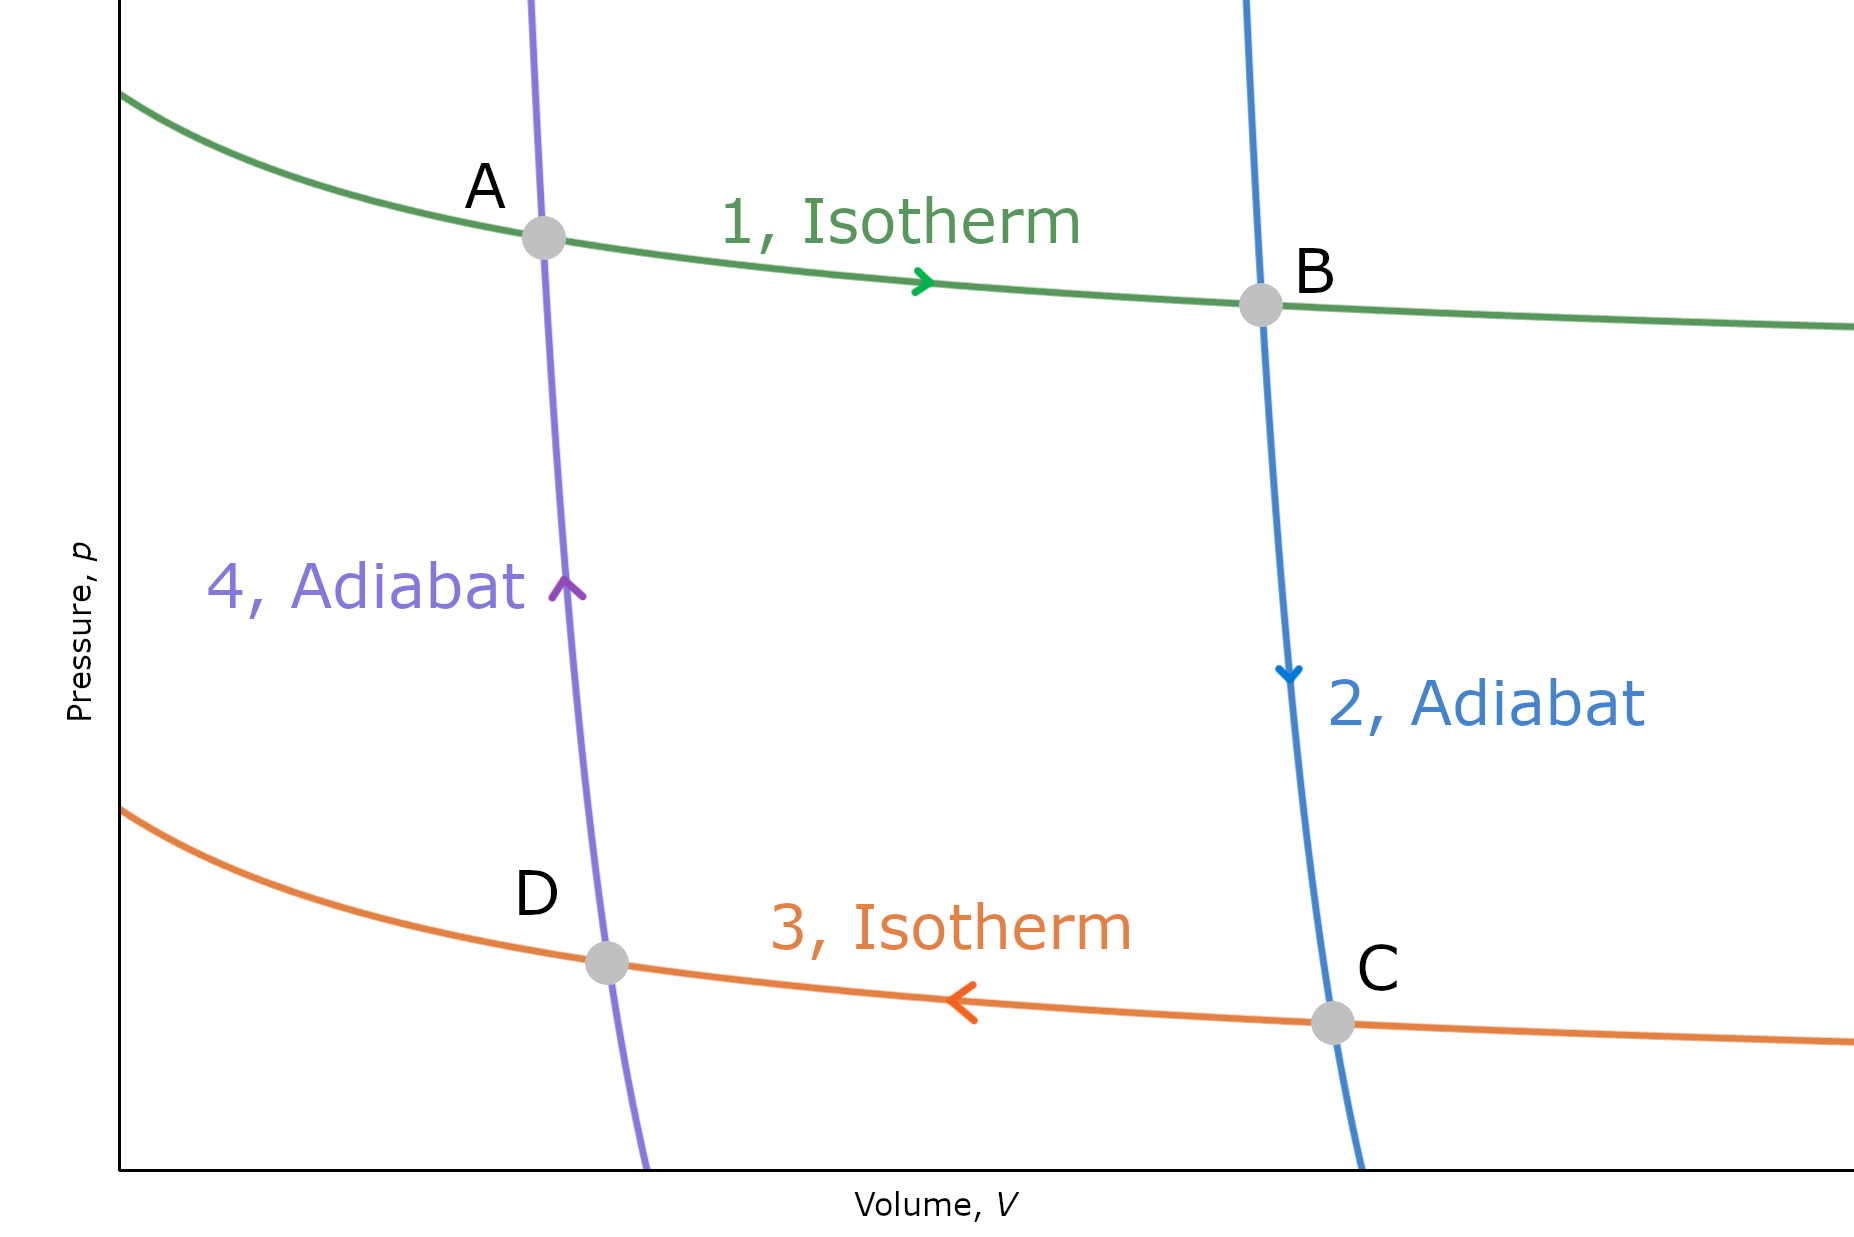
\includegraphics[scale=2]{Images/CarnotCycle.png}
            \caption{Carnot 순환}\label{f4}
        \end{figure}
        따라서 $\displaystyle\oint \difform S = \frac{q_h}{T_h} + \frac{q_c}{T_c}$이다. 이때 과정을 압력-부피 그래프로 나타내면 Figure \ref{f4}와 같다.
        \par 이때 1번과 3번 과정은 등온 과정이므로, $\displaystyle q_h = nRT_h \ln{\frac{V_B}{V_A}}$와 $\displaystyle q_c = nRT_c \ln{\frac{V_D}{V_C}}$를 만족한다. 
        또한, 2번과 4번 과정은 단열 과정이므로 4번 과정에서 $\displaystyle V_A {T_h}^c = V_D {T_c}^c$가, 
        2번 과정에서 $\displaystyle V_B {T_h}^c = V_C {T_c}^c$를 만족한다. 이 둘을 곱하면 다음을 만족한다:
        \begin{equation*}
            V_A V_C {T_h}^c {T_c}^c = V_B V_D {T_h}^c {T_c}^c
        \end{equation*}
        따라서 $\displaystyle V_D / V_C = V_A / V_B$를 만족한다. 따라서 다음을 만족한다:
        \begin{equation*}
            q_c = nRT_c \ln{\frac{V_D}{V_C}} = nRT_c \ln{\frac{V_A}{V_B}} = -nRT_c \ln{\frac{V_B}{V_A}}
        \end{equation*}
        따라서 
        \begin{obs}\label{carnotc}
        \begin{equation*}
            \frac{q_h}{q_c} = -\frac{nRT_h \ln{V_B / V_A}}{-nRT_c \ln{V_B / V_A}} = -\frac{T_h}{T_c}
        \end{equation*}
        \end{obs}
        이므로,
        \begin{equation*}
            \frac{q_h}{T_h} + \frac{q_c}{T_c} = 0
        \end{equation*}
        을 만족한다. 따라서 Carnot 순환에서 $\oint \difform S = 0$을 만족한다. 
        \end{proof}
        \par 열기관의 \textbf{효율(Efficiency, $\eta$)}는 다음과 같이 정의된다:
        \begin{defn}[열기관의 효율]
        \begin{equation*}
            \eta = \frac{\left\vert w \right\vert}{\left\vert q_h \right\vert}
        \end{equation*}
        \end{defn}
        이때 $w$는 열기관이 한 일, $q_h$는 고열원에서 흡수한 열에너지이다. 열기관이 고열원에서 흡수한 열에너지는 일과 저열원으로 방출한 열에너지로 전환되므로, 
        \begin{equation*}
            \eta = \frac{\left\vert q_h \right\vert - \left\vert q_c \right\vert}{\left\vert q_h \right\vert} = 1 - \frac{\left\vert q_c \right\vert}{\left\vert q_h \right\vert}
        \end{equation*}
        로도 쓸 수 있다. Carnot 순환을 하는 열기관에서는 등식 \ref{carnotc}에 의해
        \begin{obs}[Carnot 순환을 하는 열기관의 효율]
        \begin{equation*}
            \eta = 1 - \frac{T_c}{T_h}
        \end{equation*}
        \end{obs}
        로 표현할 수 있다.
        \par 열역학 제2 법칙에 의해, \textit{모든 가역적 열기관은 같은 효율을 가진다.} 
        \begin{proof}
        고열원에서 열에너지를 받아 일을 하는 가역적 열기관 A와 
        저열원에서 열에너지를 받고 A로부터 일을 받아 고열원으로 열에너지를 방출하는 가역적 열기관 B를 가정한다. 이때 A의 효율이 더 높다고 가정하면, '남는 일'이 존재하게 
        된다. 따라서 이 경우 고열원에서 받은 열에너지와 저열원으로 방출하는 열에너지의 차를 모두 '남는 일'로 전환하는 열기관이 된다. 이는 열역학 제2 법칙에 모순이므로, 
        모든 가역적 열기관은 같은 효율을 가진다고 할 수 있다.
        \end{proof}
        \par 모든 열역학 과정은 여러 Carnot 순환의 합으로 근사할 수 있다. 따라서 엔트로피는 상태함수임을 확인할 수 있다.
        \par 온도 $T_h$인 고열원에서 효율 $\eta$의 일을 하고 온도 $T$인 저열원으로 열을 방출하는 가역적 열기관은 다음과 같은 등식을 만족한다:
        \begin{equation*}
            T = \left( 1- \eta\right)T_h
        \end{equation*}
        이를 통해 \textbf{열역학적 온도(Thermodynamic temperature scale)}를 정의할 수 있고, 단위는 K(켈빈, Kelvin)이다.\footnote[11]{%
        2019년에 "Boltzmann 상수를 $1.380\,649 \times 10^{-23}$ J K$^{-1}$로 한다."로 정의되었다.}
        \par 내부 에너지로부터, $\difform U = \difform q + \difform w = \difform q_\mathrm{rev} + \difform w_\mathrm{rev}$ 이므로 
        $\difform q_\mathrm{rev} - \difform q = \difform w - \difform w_\mathrm{rev}$임을 확인할 수 있다. 이때 
        $\difform w - \difform w_\mathrm{rev} \geq 0$이므로, $\difform q_\mathrm{rev} - \difform q \geq 0$이다. 따라서 
        $\displaystyle \difform q_\mathrm{rev} \geq \difform q$이다. 따라서 다음 부등식을 만족한다(\textbf{Clausius 부등식(Clausius inequality)}):
        \begin{law}[Clausius 부등식]\label{clausiusineq}
        \begin{equation*}
            \difform S \geq \frac{\difform q}{T}
        \end{equation*}
        \end{law}
        고립계에서 $\difform q = 0$이므로, \textbf{고립계에서 자발적 변화가 일어날 때 엔트로피는 감소하지 않는다.} 또한, 총 엔트로피에 대해 
        $\difform S_\mathrm{tot} = \difform S + \difform S_\mathrm{sur} \geq 0$을 만족한다. 이때 $\difform S_\mathrm{tot} > 0$, 즉 
        자발적 과정일 때 이는 비가역적 과정이다. 또한, $\difform S_\mathrm{tot} = 0$, 즉 가역적 과정일 때에는 평형 상태에 있다.
        \par 고열원에서 저열원으로 열이 흐르는 과정에서,
        \begin{equation*}
            \difform S \geq \frac{\difform q_h}{T_h} + \frac{\difform q_c}{T_c}
        \end{equation*}
        를 만족한다. 따라서 $\displaystyle\difform q_h = -\difform q_c$이므로,
        \begin{equation*}
            \difform S \geq \left( \frac{1}{T_c} - \frac{1}{T_h} \right)\difform q_c > 0
        \end{equation*}
        을 만족한다. 따라서 열이 온도가 높은 곳에서 온도가 낮은 곳으로 흐르는 것은 자연스럽다.
    \section{열역학 과정에서의 엔트로피 변화}
        \hspace{\parindent} 만약 이상 기체에서 등온 팽창이 가역적으로 일어난다면, $\displaystyle\Delta S = nR \ln{\frac{V_f}{V_i}}$임을 보였다. 또한 가역 과정이므로, $\Delta S_\mathrm{tot} = 0$에서 
        $\displaystyle\Delta S = -nR \ln{\frac{V_f}{V_i}}$임을 보일 수 있다. 만약 등온 팽창이 자유 팽창으로 일어난다면($p_\mathrm{ex} = 0$), $w=0$이고 $\Delta U = 0$에서 
        $q=0$, 즉 $\Delta S_\mathrm{sur} = 0$이다. 따라서 총 엔트로피 변화량은 $\displaystyle\Delta S_\mathrm{tot} = nR \ln{\frac{V_f}{V_i}}$이다. 
        이 또한 $\Delta S > 0$을 만족하고, 따라서 비가역 과정임을 알 수 있다.
        \par 상태 변화에서 또한 엔트로피 변화를 측정할 수 있다. \textbf{정상 상태 변화 온도(Normal transition temperature, $T_\mathrm{trs}$)}는 두 상이 1 atm에서 
        평형을 이루는 온도이다. 이때 $q = \Delta_{\mathrm{trs}}H$이므로, 몰 엔트로피 변화는 다음과 같이 정의된다: 
        \begin{defn}[상태 변화의 몰 엔트로피 변화]\label{trsentr}
        \begin{equation*}
            \Delta_{\mathrm{trs}}S = \frac{\Delta_\mathrm{trs}H}{T_\mathrm{trs}}
        \end{equation*}
        \end{defn}
        만약 상태 변화가 발열 반응일 경우, $\Delta S < 0$이고 흡열 반응일 경우 $\Delta S > 0$이다. 다만 이 경우 $\Delta S_\mathrm{sur}$의 부호는 $\Delta S$의 부호와 
        반대이다. $T_\mathrm{trs}$에서, $\Delta S_\mathrm{tot} = 0$이다. 기화 엔트로피 $\Delta_\mathrm{vap}S^{\circlehbar} \approx 85$ J K$^{-1}$ mol$^{-1}$이다. 
        이를 \textbf{Trouton의 법칙(Trouton's rule)}이라 부르며, 이는 경험적으로 얻어진다. 이는 기화 시에 부피 변화가 물질에 상관없이 비슷하기 때문이라고 설명한다. 
        그러나 여기에서 벗어나는 경우도 존재하는데, 이는 분자 간 인력이 크기 때문에 액체 상태에서 분자의 부분적인 '질서도'가 있기 때문이라고 설명한다.
        \par 엔트로피의 정의에 따라, $\displaystyle S\left(T_f\right) = S\left(T_i\right) + \int_{T_i}^{T_f}\frac{\difform q_\mathrm{rev}}{T}$가 성립하고, 등압 조건에서 
        $\difform q_\mathrm{rev} = \difform H$가 성립하므로 $\difform H = C_p \difform T$에서 다음이 성립한다:
        \begin{cor}[등압 조건에서의 엔트로피]\label{entisobar}
        \begin{equation*}
            S\left(T_f\right) = S\left(T_i\right)+\int_{T_i}^{T_f}\frac{C_p\difform T}{T}
        \end{equation*}
        \end{cor}
        만약 $C_p$가 온도에 무관하다면, 
        \begin{equation*}
            S\left(T_f\right)=S\left(T_i\right) + C_p\int_{T_i}^{T_f}\frac{\difform T}{T} = S\left(T_i\right)+C_p \ln{\frac{T_f}{T_i}}
        \end{equation*}
        가 성립한다. 만약 부피가 일정하고 $C_V$가 온도에 무관하다면, 
        \begin{equation*}
            S\left(T_f\right) = S\left(T_i\right) + C_V \ln{\frac{T_f}{T_i}}
        \end{equation*}
        가 성립한다. 경로가 복잡할 경우 여러 경로로 나누어 생각할 수 있다.
    \section{엔트로피의 측정}
        \hspace{\parindent} 엔트로피는 열량계를 통해 측정된 열 출입을 이용하여 계산될 수 있다. 이때 \textbf{표준 엔트로피(Standard entropy, $S^\circlehbar\left(T\right)$)}는 
        이렇게 계산된 순수한 물질의 1 bar일 때의 엔트로피이다. 
        또한, \textbf{표준 몰 엔트로피(Standard molar entropy, $S_{m}^{\circlehbar}\left(T\right)$)}는 이를 물질의 몰수로 나누어 구한다. 
        \par $T=0$에서 열용량을 구하기 어렵기 때문에, 비금속 고체의 경우 열용량이 $T^3$에 비례한다는 \textbf{Debye 외삽(Debye extrapolation)}을 이용할 수 있다. 이는 
        $C_{p,m} = aT^3$으로 열용량을 근사함으로써, 엔트로피를 추정할 수 있게 한다.
        \par 열역학 제3 법칙은 다음과 같이 기술된다:
        \begin{law}[열역학 제3 법칙]
            모든 완전한 결정은 $T=0$일 때 $S=0$이다. 
        \end{law}
        또한, Walther Hermann Nernst는 다음과 같은 이론을 세웠다:
        \begin{thm}[Nernst 열 이론(Nernst heat theorem)]
            모든 물리적/화학적 변화는 절대 온도가 0으로 수렴할수록 그 과정에 참여하는 모든 물질이 완전히 정렬될 때 그 엔트로피 변화가 0으로 수렴한다.
        \end{thm}
        \par 만약 결정의 배열이 달라질 수 있을 경우, 가능한 미시상태의 수는 1보다 커질 수 있다($\displaystyle\mathcal{W}>0$). 따라서 이때 엔트로피는 0이 아닐 수 있는데, 이를 \textbf{잔류 엔트로피(Residual entropy)}라 한다. 
        얼음 결정은 $3.4$ J K$^{-1}$ mol$^{-1}$의 잔류 엔트로피를 가진다.
        \par 열역학 제3 법칙에 의한 엔트로피 변화는 \textbf{제3 법칙 엔트로피(Third-law entropy)}, 또는 \textbf{엔트로피(Entropy)}라 부른다. 
        \textbf{표준 반응 엔트로피(Standard reaction entropy, $\Delta_r S^{\circlehbar}$)}는 다음과 같이 정의된다:
        \begin{defn}[표준 반응 엔트로피]
        \begin{equation*}
            \Delta_r S^{\circlehbar} = \sum_{\textrm{생성물}} \nu S_m^{\circlehbar} - \sum_{\textrm{반응물}} \nu S_m^{\circlehbar}
        \end{equation*}
        \end{defn}
        또는 화학종 J에 대해 다음과 같이 쓸 수 있다:
        \begin{equation*}
            \Delta_r S^{\circlehbar} = \sum_{\mathrm{J}} \nu_{\mathrm{J}}S_m^{\circlehbar}\left(\mathrm{J}\right)
        \end{equation*}
        이온에 대해서는, $S^{\circlehbar}\left(\textrm(H)^{+},\textrm{aq}\right)=0$으로 관습적으로 정의한다.
        \par 식 \ref{entisobar}에 의해, 엔트로피는 온도 의존성을 가진다. 또한 다음과 같이 표현할 수 있다:
        \begin{cor}
        \begin{equation*}
            \Delta_r S^{\circlehbar}\left(T_2\right) = \Delta_r S^{\circlehbar}\left(T_1 \right)+\int_{T_1}^{T_2}\frac{\Delta_r C_p^{\circlehbar}}{T}\difform T
        \end{equation*}
        \end{cor}
        이때 $\displaystyle\Delta_r C_p^{\circlehbar} = \sum_{\mathrm{J}}\nu_\mathrm{J}C_{p,m}^{\circlehbar}\left(\mathrm{J}\right)$로 정의된다. 이는 Kirchhoff의 법칙(식 \ref{kirlaw})과 
        유사하다. 만약 $\Delta_r C_p^{\circlehbar}$가 온도에 무관하다면, 다음이 성립한다:
        \begin{equation*}
            \Delta_r S^{\circlehbar}\left(T_2\right) = \Delta_r S^{\circlehbar}\left(T_1\right) + \Delta_r C_p^{\circlehbar} \ln{\frac{T_2}{T_1}}
        \end{equation*}
    \section{계에서만 생각하기}\label{ch3sub4}
        \hspace{\parindent} 엔트로피를 계의 상태를 나타내는 변수들로만 나타내기 위해, \textbf{Helmholtz 에너지(Helmholtz energy)}와 \textbf{Gibbs 에너지(Gibbs energy)}라는 새로운 
        에너지를 도입한다. 이는 Clausius 부등식(\ref{clausiusineq})으로부터 출발한다:
        \begin{equation*}
            \difform S - \frac{\difform q}{T} \geq 0
        \end{equation*}
        등적 과정을 가정하면, $\difform q_V = \difform U$가 되어 다음을 만족한다:
        \begin{equation*}
            \difform S - \frac{\difform U}{T} \geq 0
        \end{equation*}
        엔트로피와 내부 에너지 모두 상태 함수이므로, 다음을 만족한다:
        \begin{cor}\label{helmspon}
        \begin{equation*}
            T \difform S \geq \difform U
        \end{equation*}
        \end{cor}
        한편 등압 과정을 가정하면, $\difform q_p = \difform H$를 만족하므로 마찬가지로 다음을 만족한다:
        \begin{cor}\label{gibbspon}
        \begin{equation*}
            T \difform S \geq \difform H
        \end{equation*}
        \end{cor}
        이를 다루기 위해 \textbf{Helmholtz 에너지, $A$}를 다음과 같이 정의한다:
        \begin{defn}[Helmholtz 에너지]
        \begin{equation*}
            A = U - TS
        \end{equation*}
        \end{defn}
        또한, \textbf{Gibbs 에너지, $G$}를 다음과 같이 정의한다:
        \begin{defn}[Gibbs 에너지]
        \begin{equation*}
            G = H - TS
        \end{equation*}
        \end{defn}
        \par 식 \ref{helmspon}을 만족하기 위해서는 $\difform A_{T,V} \leq 0$을, 식 \ref{gibbspon}을 만족하기 위해서는 $\difform G_{T,V} \leq 0$을 만족해야 한다. 
        이때 Helmholtz 에너지는 등온 조건에서 계가 할 수 있는 최대 일에 해당한다. 이는 다음과 같이 증명된다:
        \begin{proof}
        \par $\difform U = \difform q + \difform w$에서, Clausius 부등식 (\ref{clausiusineq})으로부터 $\difform S \geq \difform q/T$를 취하면,
        $\difform U \leq T\difform S + \difform w$를 만족한다. 따라서 $\difform w \geq \difform U -T\difform S$를 만족하고, 따라서 다음을 만족한다:
        \begin{equation*}
            \difform w_{\mathrm{max}} = \difform U - T \difform S
        \end{equation*}
        따라서 등온 조건에서 다음을 만족한다:
        \begin{equation*}
            \difform w_\mathrm{max} = \difform A
        \end{equation*}
        \end{proof}
        마찬가지로, Gibbs 에너지는 등온·등압 조건에서 최대 \textbf{추가 일(Additional work)}에 해당한다. 이는 $\difform G = \difform q + \difform w + \difform \left(pV\right) - T\difform S$라는 
        사실과 $\difform w_\mathrm{rev} = -p\difform V + \difform w_\mathrm{add,max}$라는 사실로부터 유도된다.
        \par \textbf{표준 반응 Gibbs 에너지(Standard Gibbs energy of reaction)}는 다음과 같이 정의된다:
        \begin{defn}[표준 반응 Gibbs 에너지]
        \begin{equation*}
            \Delta_r G^{\circlehbar} = \Delta_r G^\circlehbar - T\Delta_r S^\circlehbar
        \end{equation*}
        \end{defn}
        또한, \textbf{표준 생성 Gibbs 에너지(Standard Gibbs energy of formation, $\Delta_r G^\circlehbar$)}는 표준 상태의 원소로부터 그 화학종이 생성될 때의 표준 반응 Gibbs 에너지에 해당한다. 엔탈피에서와 
        마찬가지로, 표준 반응 Gibbs 에너지는 다음과 같이 쓸 수 있다:
        \begin{defn}[표준 반응 Gibbs 에너지]
        \begin{equation*}
            \Delta_r G^\circlehbar = \sum_{\mathrm{J}}\nu_\mathrm{J}\Delta_f G^\circlehbar\left(\mathrm{J}\right)
        \end{equation*}
        \end{defn}
        이온의 경우, $\displaystyle\Delta_f G^\circlehbar \left(H^{+},\mathrm{aq}\right) = 0$으로 정의한다.
        \par 이온의 용매화 Gibbs 에너지는 \textbf{Born 방정식(Born equation)}으로 추정할 수 있다:
        \begin{law}[Born 방정식]
        \begin{equation*}
            \Delta_\mathrm{solv}G^\circlehbar = -\frac{{z_i}^2 e^2 N_A}{8 \pi \varepsilon_0 r_i}\left( 1-\frac{1}{\epsilon_r}\right)
        \end{equation*}
        \end{law}
        이는 개별 이온을 구형으로 간주하고 수화 반지름 $r_i$와 이온의 전하량 $z_i$, 용매의 비유전율 $\varepsilon_r$에 대해 전기 퍼텐셜을 계산한 것이다.
    \section{열역학 제1 법칙과 제2 법칙을 합친다면?}\label{dudhdadg}
        내부 에너지의 Legendre 변환(Legendre transformation)으로부터 다음 네 개의 식이 성립한다:
        \begin{table}[H]
        \centering
            \begin{tabular}{ c c c }
                \hline
                \rowcolor{lightgray}
                상태함수& &식\\
                \hline
                $\difform U$ & $=$ & $T \difform S - p\difform V$ \\
                $\difform H$ & $=$ & $T \difform S + V\difform p$ \\
                $\difform A$ & $=$ & $-p \difform V - S \difform T$ \\
                $\difform G$ & $=$ & $V\difform p - S \difform T$ \\
                \hline
            \end{tabular}
        \end{table}
        위 식 네 개는 완전미분(\ref{exactdiff} 참고)이므로, 다음 \textbf{Maxwell 관계(Maxwell relation)}가 성립한다:
        \begin{table}[H]
        \centering
            \begin{tabular}{ c|c c c }
                \hline
                \rowcolor{lightgray}
                상태함수& &식& \\
                \hline
                $U$ & $\displaystyle \left(\frac{\partial T}{\partial V}\right)_S$ & $\displaystyle =$ & $\displaystyle -\left(\frac{\partial p}{\partial S}\right)_V$ \\
                $H$ & $\displaystyle \left(\frac{\partial T}{\partial p}\right)_S$ & $\displaystyle =$ & $\displaystyle \left(\frac{\partial V}{\partial S}\right)_p$ \\
                $A$ & $\displaystyle \left(\frac{\partial p}{\partial T}\right)_V$ & $\displaystyle =$ & $\displaystyle \left(\frac{\partial S}{\partial V}\right)_T$ \\
                $G$ & $\displaystyle \left(\frac{\partial V}{\partial T}\right)_p$ & $\displaystyle =$ & $\displaystyle -\left(\frac{\partial S}{\partial p}\right)_T$ \\
                \hline
            \end{tabular}
        \end{table}
        이를 이용하면 내부 압력 $\pi_T = \left(\frac{\partial U}{\partial V}\right)_T$가 다음과 같음을 보일 수 있다:
        \begin{equation*}
            \begin{aligned}
                \pi_T &= \left(\frac{\partial U}{\partial V}\right)_T\\
                &= \left(\frac{\partial U}{\partial S}\right)_V \left(\frac{\partial S}{\partial V}\right)_T + \left(\frac{\partial U}{\partial V}\right)_S\\
                &= T\left(\frac{\partial S}{\partial V}\right)_T -p\\
                &= T\left(\frac{\partial p}{\partial T}\right)_V -p
            \end{aligned}
        \end{equation*}
        \par Gibbs 에너지에서 다음 두 식이 성립한다:
        \begin{cor}\label{gibbspartial}
        \begin{align*}
            \left(\frac{\partial G}{\partial T}\right)_p &= -S\\
            \left(\frac{\partial G}{\partial p}\right)_T &= V
        \end{align*}
        \end{cor}
        \par 또한, Gibbs 에너지의 정의($G = H - TS$)에서 다음이 성립한다:
        \begin{equation*}
            \left(\frac{\partial G}{\partial T}\right)_p = \frac{G-H}{T}
        \end{equation*}
        이때 다음이 성립한다:
        \begin{equation*}
            \begin{aligned}
                \left(\frac{\partial G/T}{\partial T}\right)_p &= \frac{1}{T}\left(\frac{\partial G}{\partial T}\right)_p -\frac{G}{T^2} \\
                &= \frac{G-H}{T^2}-\frac{G}{T^2} = -\frac{H}{T^2}
            \end{aligned}
        \end{equation*}
        따라서 다음 \textbf{Gibbs-Helmholtz 방정식(Gibbs-Helmholtz equation)}이 성립한다:
        \begin{law}[Gibbs-Helmholtz 방정식]\label{gheqn}
        \begin{equation*}
            \left(\frac{\partial G/T}{\partial T}\right)_p = -\frac{H}{T^2}
        \end{equation*}
        \end{law}
        이는 다음과 같이 쓸 수 있다:
        \begin{cor}
        \begin{equation*}
            \left(\frac{\partial \Delta G/T}{\partial T}\right)_p = -\frac{\Delta H}{T^2}
        \end{equation*}
        \end{cor}
        \par 등온 과정에서, Gibbs 에너지는 다음과 같은 식을 만족한다:
        \begin{equation*}
            G_m\left(p_f\right) = G_m\left(p_i\right)+\int_{p_i}^{p_f}V_m \difform p
        \end{equation*}
        만약 이상 기체일 경우, $V_m = RT/p$에서 다음이 성립한다:
        \begin{equation*}
            \begin{aligned}
                G_m\left(p\right) &= G_m^{\circlehbar} + RT \int_{p^\circlehbar}^{p}\frac{1}{p}\difform p\\
                &= G_m^\circlehbar + RT \ln{\frac{p}{p^\circlehbar}}
            \end{aligned}
        \end{equation*}

\chapter{순물질의 물리적 변화}
    \section{순수한 물질의 상평형도}
        \begin{defn}[상(Phase)]
            화학적 조성과 물리적 상태가 일정한 물질의 형태를 \textbf{상(Phase)}이라 한다.
        \end{defn}
        즉 고체, 액체, 기체, 또는 고체의 여러 결정상 등을 일컫는다. 상의 개수를 $P$로 나타낸다. 기체 혼합물이나 완전히 혼합된 액체 혼합물의 상의 개수는 
        $P=1$이다. \textbf{섞이지 않는(Immiscible)} 두 상이 있을 경우 이를 $P=2$로 나타내고, \textbf{섞이는(Miscible)} 하나의 상일 경우  
        $P=1$로 나타낸다. 현탁액과 같은 \textbf{분산물(Dispersion)}의 경우, 상이 두 개이므로 $P=2$이다.
        \par \begin{defn}[상태 변화]
        \textbf{상태 변화(Phase transition)}는 한 상이 다른 상으로 바뀌는 자발적 과정이다.
        \end{defn}이는 \textbf{상태 변화 온도(Transition temperature, $T_\mathrm{trs}$)}에서 일어난다. 상태 변화 온도에서는 두 상이 평형 상태를 
        이루고, 정해진 압력에서 계의 Gibbs 에너지는 최소가 된다. 상태 변화는 주로 \textbf{열분석(Thermal analysis)}을 통해 
        확인한다. 만약 상태 변화가 발열 반응일 경우, 계의 에너지를 감소시키면서 측정하면 온도 변화가 없는 구간이 나타난다. 반대로 
        상태 변화가 흡열 반응일 경우, 계의 에너지를 증가시키면서 측정하면 마찬가지로 온도 변화가 없는 구간이 나타난다. 이를 통해 
        상태 변화를 측정한다. 주로 DSC(\ref{enthal}, \ref{thermalchem} 참조)와 X선 산란 분광법이 이용된다.
        \par \begin{defn}[준안정 상]
        주어진 압력에서 가장 안정하진 않으나, 상태 변화 속도가 매우 느려 다른 상태로 거의 변하지 않는 상을 
        \textbf{준안정 상(Metastable phase)}이라 한다.
        \end{defn}
        예를 들어 다이아몬드는 흑연에 비해 1 bar에서 에너지가 높지만, 상태 
        변화에 필요한 활성화 에너지가 너무 높기 때문에 다이아몬드는 준안정 상에 해당한다.
        \par 상태 변화가 일어나기 위해서는 다음과 같은 조건을 만족해야 한다:
        \begin{rem}[상태 변화의 조건]
            평형 상태에서 물질의 화학적 퍼텐셜은 계에 있는 모든 상에 대해 같다. 
        \end{rem}
        A상과 B상이 평형을 이룬다고 할 때, A의 화학적 퍼텐셜 $\mu_\mathrm{A}$과 B의 화학적 퍼텐셜 $\mu_\mathrm{B}$에 대해 
        $\difform n$만큼 A에서 B로 변화할 때 화학적 퍼텐셜 변화는
        \begin{equation*}
            \difform G = -\mu_\mathrm{A} \difform n + \mu_\mathrm{B} \difform n = \left(\mu_\mathrm{B} - \mu_\mathrm{A}\right) \difform n
        \end{equation*}
        이다. 이 둘이 평형이므로, $\difform G = 0$이다. 따라서 $\mu_\mathrm{A} = \mu_\mathrm{B}$일 때 두 상(혹은 그 이상)이 평형을 
        이룬다.
        \par 순수한 물질의 \textbf{상평형도(Phase diagram)}는 주어진 압력과 온도에서 열역학적으로 안정한 상이 무엇인지 나타낸 그림이다. 
        상평형도에서 영역 사이의 선, 즉 \textbf{상 경계(Phase boundary)}에서는 두 상이 공존하며 평형을 이룬다. 즉 두 상의 화학적 퍼텐셜이 
        동일하다. 상평형도는 다음 Figure \ref{f5}과 같이 나타난다.
        \begin{figure}[H]
            \centering
            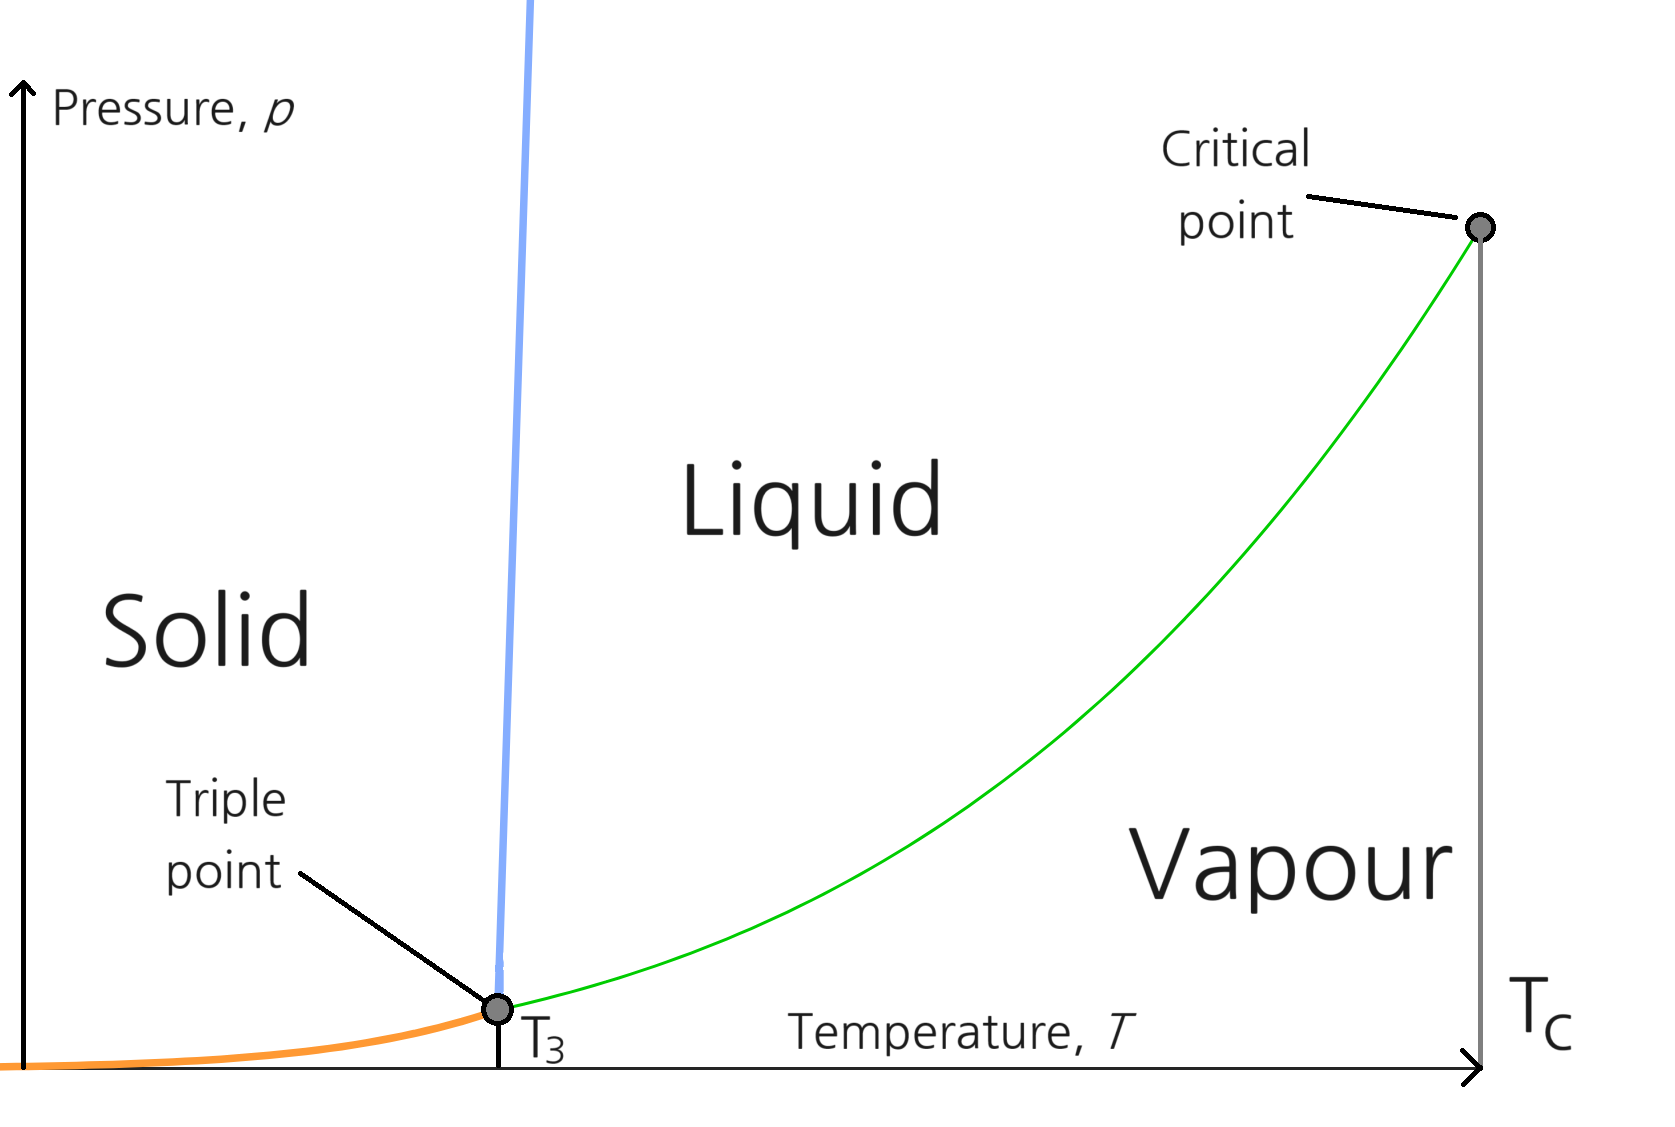
\includegraphics[scale=0.4]{Images/PhaseDiag1}
            \caption{상평형도}\label{f5}
        \end{figure}
        액체 상태의 물질은 \textbf{증기 압력(Vapour pressure)}을 가지며, 따라서 액체-기체 사이의 상 경계는 주어진 온도에서 증기 압력을 나타낸다. 
        마찬가지로, 고체-기체 상 경계는 주어진 온도에서 \textbf{승화 증기 압력(Sublimation vapour pressure)}을 나타낸다.
        \begin{defn}[액체-기체 사이의 논의]
        \begin{enum}
        \item 열린 용기에 액체가 담겨 있을 때, 외부 압력이 그 온도에서의 증기 압력보다 높다면 \textbf{증발(Vaporization, 기화라고도 함)}을 일으킨다. 
        \item 만약 외부 압력이 그 온도에서의 증기 압력과 같아진다면, 액체 전체에서 기화가 일어나는 \textbf{끓음(Boiling)}이라는 과정을 일으킨다. 
        \item 증기 압력이 외부 압력과 같아지는 지점을 \textbf{끓는점(Boiling point)}이라 한다.
        \item 외부 압력이 1 atm일 때의 끓는점을 \textbf{정상 끓는점(Normal boiling point, $T_b$)}이라 한다.
        \item 외부 압력이 1 bar일 때의 끓는점을 \textbf{표준 끓는점(Standard boiling point)}이라 한다. 일반적으로 표준 끓는점은 정상 끓는점보다 낮다.
        \end{enum}
        \end{defn}
        \begin{defn}[임계 상태와 관련한 서술]
        닫힌 용기에서 액체 상태의 물질을 가열하면 끓음이 일어나지 않는다. 대신 증기 압력이 증가하면서, 기체와 액체의 경계면이 사라지는 지점이 
        나타난다. 이때의 온도를 \textbf{임계 온도(Critical temperature, $T_c$)}라 하고, 임계 온도에서의 증기 압력을 \textbf{임계 압력(Critical pressure, $p_c$)}이라 
        한다. 이 지점 이상의 온도를 가지게 되면 물질은 하나의 균일한 상인 \textbf{초임계 유체(Supercritical fluid)}를 이룬다.
        \end{defn}
        \begin{defn}[고체-액체 사이의 논의]
        \begin{enum}
        \item 특정 압력에서 액체와 고체가 공존하면서 평형을 이루는 온도를 \textbf{녹는점(Melting temperature)}이라 한다. 
        \item 녹는점은 \textbf{어는점(Freezing temperature)}과 같다. 
        \item 1 atm에서의 어는점을 \textbf{정상 어는점(Normal freezing point, $T_f$)}이라 한다.
        \item 1 bar에서의 어는점을 \textbf{표준 어는점(Standard freezing point)}이라 한다. 
        대부분의 물질에서는 정상 어는점과 표준 어는점이 거의 일치한다. 정상 어는점은 \textbf{정상 녹는점(Normal melting point)}이라고도 한다.
        \end{enum}
        \end{defn}
        \begin{defn}[삼중점]
        세 개의 서로 다른 상이 공존하며 평형을 이루는 지점을 \textbf{삼중점(Triple point)}이라 한다. 이때의 온도를 $T_3$이라고도 나타낸다.
        \end{defn}
        순수한 물질의 삼중점은 변하지 않는다. 또한, 삼중점은 액체 상태의 물질이 존재할 수 있는 최소한의 압력에 해당한다. 또한, 고체-액체 상 경계의 
        기울기가 양수일 경우, 삼중점은 액체 상태의 물질이 존재할 수 있는 최소한의 온도에 해당한다. (예외로 물이 있다.)
        \par Josiah Willard Gibbs는 \textbf{상 규칙(Phase rule)}을 유도하였다. 각각의 변수들은 다음과 같다:
        \begin{enum}
            \item \textbf{변수(Variance, $F$)}는 자유도를 의미하며, 평형을 이루는 상의 개수를 바꾸지 않는 조건에서 자유로이 바꿀 수 있는 세기 성질의 개수를 나타낸다.
            \item \textbf{구성 성분(Constituent)}은 계를 구성하는 모든 화학종이다.
            \item \textbf{구성 요소(Component)}는 계를 구성하는 \textit{화학적으로 독립적인} 구성 성분이다.
            \item $C$는 구성 요소의 개수로, 계의 모든 상을 나타낼 수 있는 최소한의 구성 요소의 개수를 나타낸다.
        \end{enum}
        \par 먼저, 온도와 압력에 대한 자유도 2에서 시작한다. 이때 C개의 구성 요소가 있으면, 몰 분율이라는 요인에 의해 자유도가 제약된다. 
        $x_A + x_B + \cdots + x_J = 1$이므로, 구성 요소에 대해 $C-1$의 자유도가 주어진다. 이때 각 구성 요소에 대해 $P$만큼의 상이 가능하므로, 
        이 단계에서 가능한 자유도는 $P\left(C-1\right)+2$이다.
        \par 이제 평형 상태를 생각하자. $P$개의 상이 평형을 이룰 때, 화학 퍼텐셜은 $P$개의 상 모두에서 같아야 한다. 따라서 이때 감소되는 
        자유도는 $P-1$이고, $C$개의 구성 요소에 대해 이러한 자유도가 모두 감소되므로 가능한 자유도는 $P\left(C-1\right)-C\left(P-1\right) + 2$, 즉 
        $F = C - P + 2$를 만족한다.
        \par 따라서 Gibbs의 상 규칙은 다음과 같다:
        \begin{law}[상 규칙]
        \begin{equation*}
            F = C- P +2
        \end{equation*}
        \end{law}
        만약 구성 요소가 하나일 경우($C=1$), $F = 3-P$를 만족한다. 따라서 이때에는 상이 하나일 때 독립변수는 두 개, 상이 두 개일 때 독립변수는 하나, 
        상이 세 개(삼중점)일 때 독립변수는 없다. 이를 계가 \textbf{불변(Invariant)}이라 한다. 
        추가적으로, 구성 요소가 하나일 경우에는 네 개의 상이 공존하면서 평형을 이루는 점은 존재할 수 없다.
        \par \ref{phasethermo}에서 다루겠지만, 물을 비롯한 몇몇 물질에서는 고체-액체 상 경계의 기울기가 음수로 나타난다. 특히 물에서는 얼음 I 상의 빈 공간이 
        물일 때보다 많기 때문에 액체에서 얼음 I로 응고되면 부피가 증가한다. 또한, 헬륨-4의 경우 액체 상태가 2종류 존재한다. 이 두 액체의 $\displaystyle C_{p,m}$을 비교하면 불연속점이 
        나타난다. 이를 람다-상태 변화($\lambda$-transition)라 한다. 헬륨-II 액체 상태의 경우 \textbf{초유체(Superfluid)} 상태로, 점성이 0인 특성을 보인다.
    \section{상의 열역학적 관점}\label{phasethermo}
        \hspace{\parindent} 다음이 성립함은 \ref{dudhdadg}에서 살펴보았다:
        \begin{equation*}
            \difform G = V\difform p-S\difform T
        \end{equation*}
        각각에서, $\mu = G_m$이라는 사실을 이용하면 다음이 성립한다:
        \begin{equation*}
            \begin{aligned}
                \left(\frac{\partial \mu}{\partial T}\right)_p &= -S_m \\
                \left(\frac{\partial \mu}{\partial p}\right)_T &= V_m
            \end{aligned}
        \end{equation*}
        이때, $T>0$이면 $S_m>0$이므로, 온도가 증가할수록 화학 퍼텐셜은 감소한다. 
        일반적으로 $S_m\left(\mathrm{g}\right)>S_m\left(\mathrm{l}\right)>S_m\left(\mathrm{s}\right)$이므로, 화학 퍼텐셜의 기울기의 절댓값은 
        고체에서보다 액체에서, 액체에서보다 기체에서 더 크다.
        \par 또한, $V_m>0$에서 압력이 증가하면 화학 퍼텐셜은 증가한다. 대부분의 경우에서, $V_m\left(\mathrm{l}\right)>V_m\left(\mathrm{s}\right)$이므로 
        압력이 증가할 때 화학 퍼텐셜이 증가하는 정도는 고체에서보다 액체에서가 더 크다. 따라서 이 경우 압력이 증가하면 어는점이 올라간다. 
        그러나 물과 같은 일부 경우에서는 $V_m\left(\mathrm{l}\right)< V_m\left(\mathrm{s}\right)$이므로, 
        압력이 증가할 때 화학 퍼텐셜이 증가하는 정도는 액체에서보다 고체에서가 더 크다. 따라서 이 경우 압력이 증가하면 어는점이 내려간다.
        \par 액체나 고체 등에 비활성 기체(Inert gas)를 이용하여 압력을 가했을 때, 압력을 받는 물체의 증기 압력은 증가한다. 따라서 
        \textbf{부분 증기 압력(Partial vapour pressure)}을 정의할 수 있고, 이는 전체 압력 $P$와 관련이 있다. 
        위에서 언급한 것과 같이, $\displaystyle\left(\frac{\partial \mu}{\partial p}\right)_T = V_m$이 성립하므로, 증기를 이상 기체로 가정하면 
        $\displaystyle\difform \mu = V_m \difform p = RT \difform p /p$가 성립한다. 또한, 증기와 응축 상태(액체로 가정하겠다)가 평형을 이루므로, 다음이 성립한다: 
        $$
        \difform \mu\left(\mathrm{l}\right) = V_m\left(\mathrm{l}\right)\difform p 
        = \difform \mu\left(\mathrm{g}\right) = \frac{RT \difform p}{p}
        $$
        따라서, \underline{이때 불활성 기체는 증기와 상호작용하지 않고 액체에 녹지 않는다고 가정하면}\footnote[12]{%
        이 가정이 없을 경우 굉장히 복잡해진다.}, 정상 증기 압력 $p^\ast$와 액체에 추가로 가해진 압력 $\Delta P$에 대해 $p^\ast + \Delta p = p$라 
        가정할 때, 다음이 성립한다(단 이때 적분변수는 $p^\prime$으로 한다):
        \begin{equation*}
            RT \int_{p^\ast}^{p}\frac{\difform {p^\prime}}{p^{\prime}} = \int_{p^\ast}^{p^\ast + \Delta P}V_m\left(\mathrm{l}\right)\difform P
        \end{equation*}
        따라서 다음이 성립한다:
        \begin{equation*}
            \ln{\frac{p}{p^\ast}}=\frac{V_m\left(\mathrm{l}\right)}{RT}\Delta P
        \end{equation*}
        즉 $p=p^\ast e^{V_m\left(\mathrm{l}\right)\Delta P/RT}$가 성립한다.
        \par 상 $\alpha$와 상 $\beta$가 압력 $p$, 온도 $T$에서 평형을 이룰 때, 이 둘의 화학 퍼텐셜 $\mu$가 같음은 위에서 살펴보았다. 
        이제 상 경계의 기울기를 구할 것이다. $\mu = G_m$이라는 사실로부터 출발하자. 
        $\difform G_m = V_m \difform p - S_m \difform T$에서, 
        \begin{equation*}
            V_m \left(\alpha\right)\difform p - S_m \left(\alpha\right)\difform T = V_m \left(\beta\right)\difform p - S_m \left(\beta\right)\difform T
        \end{equation*}
        이 성립한다. 따라서 
        \begin{equation*}
            \left\{S_m\left(\beta\right) - S_m\left(\alpha\right)\right\}\difform T = \left\{V_m\left(\beta\right) - V_m\left(\alpha\right)\right\}\difform p
        \end{equation*}
        가 성립하고, 이를 정리하면 다음과 같다:
        \begin{equation*}
            \Delta_\mathrm{trs} S \difform T = \Delta_\mathrm{trs}V\difform p
        \end{equation*}
        따라서 다음과 같은 \textbf{Clapeyron 등식(Clapeyron equation)}을 유도할 수 있다:
        \begin{law}[Clapeyron 등식]
        \begin{equation*}
            \frac{\difform p}{\difform T} = \frac{\Delta_\mathrm{trs}S}{\Delta_\mathrm{trs}V}
        \end{equation*}
        \end{law}
        압력이 변화하는 조건에서는 각각의 "역수"를 취하면 된다.
        \par 식 \ref{trsentr}에 의해, 고체-액체 상 경계에서도 다음이 성립한다:
        \begin{equation*}
            \frac{\difform p}{\difform T} = \frac{\Delta_\mathrm{fus}H}{T \Delta_\mathrm{fus}V}
        \end{equation*}
        따라서 $\difform T$를 우변으로 넘기고 양변을 적분하면 다음과 같다:
        \begin{equation*}
            \int_{p^\ast}^{p}\difform p = \frac{\Delta_\mathrm{fus}H}{\Delta_\mathrm{fus}V}\int_{T^\ast}^{T}\frac{\difform T}{T}
        \end{equation*}
        따라서 다음이 성립한다:
        \begin{equation*}
            p = p^\ast + \frac{\Delta_\mathrm{fus}H}{\Delta_\mathrm{fus}V}\ln{\frac{T}{T^\ast}}
        \end{equation*}
        이때 $\displaystyle \ln{\frac{T}{T^\ast}} = \ln{\left(1+\frac{T-T^\ast}{T^\ast}\right)}\approx \frac{T-T^\ast}{T^\ast}$으로 근사할 수 있으므로, 
        다음과 같이 일차식으로 근사할 수 있다:
        \begin{equation*}
            p = p^\ast + \frac{\Delta_\mathrm{fus}H}{T^\ast \Delta_\mathrm{fus}V}\left(T-T^\ast \right)
        \end{equation*}
        \par 액체-기체 상 경계에서도 비슷하게 성립한다. 이때 기체의 부피가 액체의 부피보다 현저히 크기 때문에, $\Delta_\mathrm{vap}V \approx V_m\left(\mathrm{g}\right)$로 
        근사할 수 있다. 증기를 이상 기체로 근사하면, $V_m = RT/p$에서 
        $$
        \frac{\difform p}{\difform T} = \frac{\Delta_\mathrm{vap}H}{RT^2 /p}=\frac{p\Delta_\mathrm{vap}H}{RT^2}
        $$
        가 성립한다. 다시 정리하면 다음과 같은 \textbf{Clausius-Clapeyron 등식(Clausius-Clapeyron equation)}이 성립한다:
        \begin{law}[Clausius-Clapeyron 등식]
        \begin{equation*}
            \frac{\difform \ln{p}}{\difform T} = \frac{\Delta_\mathrm{vap}H}{RT^2}
        \end{equation*}
        \end{law}
        이 등식을 적분하면 다음과 같은 식 또한 성립한다:
        \begin{equation*}
            \ln{\frac{p}{p^\ast}} = -\frac{\Delta_\mathrm{vap}H}{R}\left(\frac{1}{T} - \frac{1}{T^\ast}\right)
        \end{equation*}
        \par 고체-기체 상 경계에서도 같은 과정을 통해 기울기를 구할 수 있다.

\chapter{간단한 혼합물}
    \section{열역학적 관점에서 본 혼합물}
        \hspace{\parindent}혼합물을 구성하는 물질 $J$에 대해, 부분 몰 부피 $V_J$를 다음과 같이 정의한다:
        \begin{defn}[부분 몰 부피]
        \begin{equation*}
            V_J = \left(\frac{\partial V}{\partial n_J}\right)_{p,T,n^\prime}
        \end{equation*}
        \end{defn}
        이때 $n^\prime$은 혼합물의 다른 모든 물질의 몰수가 일정함을 의미한다.
        \par A와 B의 이원계 혼합물(Binary mixture)에서 한 물질의 몰수가 미소하게 변화할 때 부피 변화 $\difform V$는 다음과 같다:
        \begin{equation*}
            \begin{aligned}
                \difform V &= \left(\frac{\partial V}{\partial n_A}\right)_{p,T,n_B}\difform n_A + \left(\frac{\partial V}{\partial n_B}\right)_{p,T,n_A}\difform n_B\\
                &= V_A \difform n_A + V_B \difform n_B
            \end{aligned}
        \end{equation*}
        이때 $V_J$는 반드시 양수일 필요는 없다. 즉, 다른 물질을 첨가할 때 부피가 감소하는 경우도 존재한다.
        \par 혼합물에서 화학 퍼텐셜 $\mu_J$는 다음과 같이 정의된다:
        \begin{defn}[혼합물에서의 화학 퍼텐셜]
        \begin{equation*}
            \mu_J = \left(\frac{\partial G}{\partial n_J}\right)_{p,T,n^\prime}
        \end{equation*}
        \end{defn}
        A와 B의 이원계 혼합물에서 총 Gibbs 에너지는 다음과 같다:
        \begin{fact}[이원계 혼합물에서의 총 Gibbs 에너지]\label{binarygibbs}
        \begin{equation*}
            G = n_A \mu_A + n_B \mu_B
        \end{equation*}
        \end{fact}
        실제로 혼합물에서는 Gibbs 에너지가 다음과 같이 정의된다:
        \begin{defn}[혼합물에서의 Gibbs 에너지]\label{gibbsreal}
        \begin{equation*}
            \difform G = V\difform p - S\difform T + \mu_A \difform n_A + \mu_B \difform n_B + \cdots
        \end{equation*}
        \end{defn}
        이때 압력과 온도가 일정하면, $\displaystyle\difform G = \mu_A \difform n_A + \mu_B \difform n_B + \cdots = \difform w_\mathrm{add,max}$
        를 만족한다. 따라서 혼합물의 구성을 바꿔도 계에 추가적인 (비팽창) 일을 하게 된다. 조건에 따라 다음과 같이 정의할 수 있다:
        \begin{align*}
            \mu_J &= \left(\frac{\partial U}{\partial n_J}\right)_{S,V,n^\prime}\\
            \mu_J &= \left(\frac{\partial H}{\partial n_J}\right)_{S,p,n^\prime}\\
            \mu_J &= \left(\frac{\partial A}{\partial n_J}\right)_{T,V,n^\prime}
        \end{align*}
        \par A와 B의 이원계 혼합물에서 식 \ref{binarygibbs}에 의해 다음이 성립한다:
        \begin{equation*}
            \difform G = \mu_A \difform n_A + \mu_B \difform n_B + n_A \difform \mu_A + n_B \difform \mu_B
        \end{equation*}
        이때 일정한 압력과 온도에서 식 \ref{gibbsreal}를 만족해야 하므로, $n_A \difform \mu_A + n_B \difform \mu_B = 0$을 만족한다. 
        따라서 일반적인 혼합물에서 다음과 같은 \textbf{Gibbs-Duhem 등식(Gibbs-Duhem equation)}을 만족한다:
        \begin{law}[Gibbs-Duhem 등식]\label{gibbsduhem}
        \begin{equation*}
            \sum_{J} n_J \difform \mu_J = 0
        \end{equation*}
        \end{law}
        부분 몰 부피에 대해서도 유사하게, 
        \begin{equation*}
            \sum_{J} n_J \difform V_J = 0
        \end{equation*}
        을 만족한다.
        \par 이상 기체에서 $\displaystyle G_m = G_m^\circlehbar + RT\ln{\left(p/p^\circlehbar\right)}$를 만족하므로,
        \begin{law}[이상 기체에서의 화학 퍼텐셜]\label{chempotgas}
        \begin{equation*}
            \mu = \mu^\circlehbar +RT\ln{\frac{p}{p^\circlehbar}}
        \end{equation*}
        \end{law}
        를 만족한다. 이때, $p/p^\circlehbar = p$로 두자(즉 $p^\circlehbar = 1$). 
        온도와 압력이 $T$, $p$로 서로 같은 A와 B를 혼합할 때, 초기 Gibbs 에너지
        $$
        G_i = n_A \mu_A + n_B \mu_B = n_A\left(\mu_A^\circlehbar +RT\ln{p}\right) + n_B\left(\mu_B^\circlehbar + RT\ln{p}\right)
        $$
        와 최종 Gibbs 에너지
        $$
        G_f = n_A\left(\mu_A^\circlehbar +RT\ln{p_A}\right) + n_B\left(\mu_B^\circlehbar + RT\ln{p_B}\right)
        $$
        의 차 $\Delta_\mathrm{mix}G$\textbf{(혼합 Gibbs 에너지, Gibbs energy of mixing)}를 구하면
        \begin{law}[혼합 Gibbs 에너지]
        \begin{equation*}
            \Delta_\mathrm{mix}G = n_A RT \ln{\frac{p_A}{p}} + n_B RT\ln{\frac{p_B}{p}}
        \end{equation*}
        \end{law}
        가 성립한다. 이때 $n_J = x_J n$으로 치환하면 
        \begin{equation*}
            \Delta_\mathrm{mix}G = nRT \left(x_A \ln{x_A} + x_B \ln{x_B}\right)
        \end{equation*}
        가 성립한다. $x_J \leq 1$이므로, 이 경우 항상 $\Delta_\mathrm{mix}G < 0$이 성립한다. 처음 압력이 다를 경우에도 $G = \mu_A n_A + \mu_B n_B + \cdots$에서 
        시작하여 $\Delta_\mathrm{mix}G$를 유도할 수 있다.
        \par 혼합 엔트로피 $\Delta_\mathrm{mix}S$는 다음과 같이 계산할 수 있다:
        \begin{equation*}
            \Delta_\mathrm{mix}S = -\left(\frac{\partial \Delta_\mathrm{mix}G}{\partial T}\right)_p = -nR\left(x_A \ln{x_A} + x_B \ln{x_B}\right)
        \end{equation*}
        여기에서도 마찬가지로, $\ln{x} < 0$이므로 $\Delta_\mathrm{mix}S>0$이 성립한다.
        \par \textbf{이상 기체에서는 $\Delta_\mathrm{mix}H = 0$이다.}
        \par 액체와 기체가 평형을 이룰 때, 순수한 액체 A에 대해서 $\mu_A^\ast \left(\mathrm{l}\right) = \mu_A^\circlehbar \left(\mathrm{g}\right) + RT \ln{p_A^\ast}$를 
        만족한다. 
        만약 다른 물질이 A에 추가될 때, A 기체의 부분 압력 $p_A$에 대하여 평형 상태에서 다음이 성립한다:
        $$
        \mu_A \left(\mathrm{l}\right) = \mu_A^\circlehbar \left(\mathrm{g}\right) + RT \ln{p_A}
        $$
        이 두 식을 연립하면, 다음을 얻는다:
        \begin{equation*}
            \begin{aligned}
                \mu_A\left(\mathrm{l}\right) &= \mu_A^\ast\left(\mathrm{l}\right) - RT\ln{p_A^\ast}+RT\ln{p_A^\ast}\\
                &= \mu_A^\ast\left(\mathrm{l}\right) + RT\ln{\frac{p_A}{p_A^\ast}}
            \end{aligned}
        \end{equation*}
        이를 두고 François-Marie Raoult은 $p_A/p_A^\ast \approx x_A$임을 발견하였다. 따라서 다음과 같은 \textbf{Raoult 법칙(Raoult's law)}이 성립한다:
        \begin{law}[Raoult 법칙]
        \begin{equation*}
            p_A = x_A p_A^\ast
        \end{equation*}
        \end{law}
        \begin{defn}[이상 용액]
        이러한 Raoult 법칙을 모든 $x_A$ 범위에서 잘 따르는 용액을 \textbf{이상 용액(Ideal solution)}이라 한다.
        \end{defn}
        \par 이상 용액에서는 $\mu_A\left(\mathrm{l}\right) = \mu_A^\ast \left(\mathrm{l}\right) + RT \ln{x_A}$가 성립한다. 
        실제 용액에서는 Raoult 법칙을 벗어나는 경우를 많이 관찰할 수 있으나, 이 역시 $x_A \rightarrow 1$일 때에는 Raoult 법칙을 잘 따른다.
        \par 용질에 대해서는, William Henry가 다음과 같은 \textbf{Henry 법칙(Henry's law)}를 발견하였다:
        \begin{law}[Henry 법칙]
        \begin{equation*}
            p_B = x_B K_B
        \end{equation*}
        \end{law}
        이때 $K_B$는 경험적인 상수이다. $x_B \rightarrow 0$일 때 Henry 법칙을 잘 따른다.
        \begin{defn}[이상 묽은 용액]
        \par 용질이 Henry 법칙을 잘 따르고, 용매가 Raoult 법칙을 잘 따르는 용액을 \textbf{이상 묽은 용액(Ideal-dilute solution)}이라 한다.
        \end{defn}
        이 경우, 용질 분자 주변에는 거의 용매 분자뿐이므로, 용매는 거의 순수한 액체 물질로 근사할 수 있고, 용질은 용매와 다르게 거동한다. 
        (그러나 용질과 용매의 성질이 비슷할 경우 용질 또한 Raoult 법칙을 따른다.)
        \par 실제로 Henry 법칙을 이용할 때, 용질에 대해 몰랄 농도(molality) $b_B$를 이용하게 된다. 즉 $p_B = b_B k_B$로 이용한다.
    \section{용액의 성질}
        \hspace{\parindent}이상 용액에서 다음이 성립함을 보였다:
        $$
        \mu_J = \mu_J^\ast + RT \ln{x_J}
        $$
        기체에서와 마찬가지로, 액체 용액에서도 혼합 전후의 Gibbs 에너지를 계산할 수 있다. 두 액체 A와 B가 혼합될 때,
        혼합 전에는 $G_i = n_A \mu_A^\ast + n_B \mu_B^\ast$를 만족하고, 혼합 이후에는 $G_f = n_A\left(\mu_A^\ast + RT \ln{x_A}\right) + n_B\left(\mu_B^\ast + RT\ln{x_B}\right)$를 
        만족한다. 이 둘의 차 $\Delta_\mathrm{mix}G$는 다음을 만족한다:
        \begin{obs}[이상 용액의 혼합 Gibbs 에너지]\label{reggibbs}
        \begin{equation*}
            \Delta_\mathrm{mix}G=nRT\left(x_A\ln{x_A}+x_B\ln{x_B}\right)
        \end{equation*}
        \end{obs}
        이때 $n=n_A+n_B$이다. 다음 또한 만족한다:
        \begin{obs}[이상 용액의 혼합 엔트로피]
        \begin{equation*}
            \Delta_\mathrm{mix}S=-nR\left(x_A\ln{x_A} + x_B\ln{x_B}\right)
        \end{equation*}
        \end{obs}
        액체에서 또한 이상 용액에서는 $\Delta_\mathrm{mix}H = 0$을 만족하고, 나아가 
        $$
        \Delta_\mathrm{mix}V=\left(\frac{\partial \Delta_\mathrm{mix}G}{\partial p}\right)_T
        $$
        에서 
        $\Delta_\mathrm{mix}V = 0$ 또한 만족한다.
        \par 액체에서 혼합의 '동력(Driving force)'은 엔트로피 증가에 의한 것이다. 이때 $\Delta_\mathrm{mix}H=0$이라는 것은 기체에서는 
        기체 분자 사이의 상호작용이 없다는 뜻이지만, 액체에서는 A 분자끼리의 인력과 B 분자끼리의 인력의 평균 에너지가 A-B 사이의 인력과 같다는 것을 의미한다. 
        이상 용액에서 $\Delta_\mathrm{mix}G$와 $\Delta_\mathrm{mix}S$는 다음 Figure \ref{f6a}, Figure \ref{f6b}과 같이 나타난다.
        \begin{figure}[H]
            \begin{subfigure}{0.5\textwidth}
                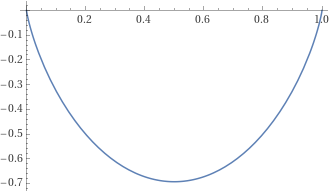
\includegraphics[width=0.9\linewidth]{Images/xlnx}
                \caption{$x$에 따른 $\Delta_\mathrm{mix}G$\footnote[1]{가로축은 $x$, 세로축은 $\Delta_\mathrm{mix}G/nRT$}}\label{f6a}
            \end{subfigure}
            \begin{subfigure}{0.5\textwidth}
                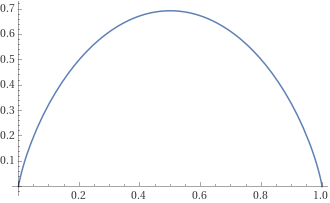
\includegraphics[width=0.9\linewidth]{Images/minusxlnx}
                \caption{$x$에 따른 $\Delta_\mathrm{mix}S$\footnote[2]{가로축은 $x$, 세로축은 $\Delta_\mathrm{mix}S/nR$}}\label{f6b}
            \end{subfigure}
        \end{figure}
        \par 실제 용액에서는 분자들 사이의 상호작용이 모두 다르다. 따라서 혼합 엔탈피가 0이 아닐 수 있고, 부피 변화 또한 0이 아닐 수 있다. 만약 
        혼합 엔트로피가 음수일 경우, 혼합의 Gibbs 에너지는 양수가 될 수 있다. 이 경우 액체의 혼합은 일어나지 않는다(Immiscible). 한편, 
        \textbf{부분적으로 섞이는(Partially miscible)} 경우도 있다. 이 경우 특정 비율까지만 혼합될 수 있다.
        \par 실제 용액과 이상 용액에서의 열역학 변수들의 차를 \textbf{초과 함수(Excess function, $X^E$)}라 한다. 이때 $X$는 열역학 변수를 의미한다. 
        초과 함수는 다음과 같이 정의된다:
        \begin{defn}[초과 함수]
        \begin{equation*}
            X^E = \Delta_\mathrm{mix}X-\Delta_\mathrm{mix}X^\mathrm{ideal}
        \end{equation*}
        \end{defn}
        예를 들어 초과 엔트로피 $S^E$를 생각할 수 있다. A와 B가 혼합될 때 초과 엔탈피 $H^E > 0$일 경우, 
        A-B 사이의 상호작용이 A-A와 B-B 사이의 상호작용보다 덜 선호된다는 것을 알 수 있다. 
        \par 이상 용액은 아니지만, 실제 용액의 좋은 모형으로 \textbf{정규 용액(Regular solution)}을 생각할 수 있다:
        \begin{defn}[정규 용액]
        정규 용액은 초과 엔탈피 $H^E \neq 0$이지만 
        초과 엔트로피 $S^E = 0$인 용액이다. 이는 두 종류의 분자가 무작위로 분포하나, 분자 간 상호작용의 크기는 같지 않은 경우로 생각할 수 있다.
        \end{defn}
        \par 정규 용액에서 초과 엔탈피는 다음과 같이 쓸 수 있다:
        \begin{obs}[정규 용액에서의 초과 엔탈피]\label{excessenth}
        \begin{equation*}
            H^E = n \xi RT x_A x_B
        \end{equation*}
        \end{obs}
        이때 $\xi$는 A-A 상호작용과 B-B 상호작용과 비교하여 A-B 상호작용의 에너지가 얼마나 되는지 나타내는 무차원 변수이다. 
        만약 $\xi<0$일 경우, A-B 상호작용이 더 선호되어 혼합은 발열 반응이 된다. 반대로 $\xi>0$일 경우, A-A와 B-B 상호작용이 더 선호되어 
        혼합은 흡열 반응이 된다. 이를 고려하여 정규 용액의 혼합 Gibbs 에너지를 구하면
        \begin{obs}[정규 용액의 혼합 Gibbs 에너지]\label{excessgibbs}
        \begin{equation*}
            \begin{aligned}
                \Delta_\mathrm{mix}G &= n\xi RT x_A x_B - T\left[-nR\left(x_A \ln{x_A}+x_B \ln{x_B}\right)\right]\\
                &= nRT\left(x_A \ln{x_A}+ x_B \ln{x_B} + \xi x_A x_B\right)
            \end{aligned}
        \end{equation*}
        \end{obs}
        과 같다. 이때 $\xi > 2$이면, $\Delta_\mathrm{mix}G$의 극소점이 두 개로 나뉜다. 이는 혼합물이 자발적으로 두 개의 상으로 나뉘는 것을 의미한다.
        \par 이제부터 용액의 총괄성(Colligative property)에 대해 살펴볼 것이다.
        \begin{defn}[총괄성]
        \textbf{총괄성(Colligative property)}이란, 용액의 물리적인 성질이 
        용질의 성질에 관계없이 용질 입자의 개수에 의존하는 것을 의미한다. 증기 압력 내림, 끓는점 오름, 어는점 내림, 삼투압이 총괄성의 예시이다.
        \end{defn}
        총괄성을 보이기 위해서는 두 가지 가정이 필요하다:
        \begin{enum}
            \item 용질은 비휘발성이다. 즉 용질은 증기 압력에 관여하지 않는다.
            \item 용질은 고체 용매에 녹지 않는다. 즉 용매가 응고하면 순수한 고체 물질이 된다. 
        \end{enum}
        총괄성은 액체 용매에 용질이 녹을 때 액체의 화학 퍼텐셜이 감소하는 것으로부터 출발한다. 이상 용액에서(즉 Raoult 법칙을 만족하면), 순수한 액체 용매의 
        화학 퍼텐셜 $\mu_A^\ast$에서 용질이 녹으면 화학 퍼텐셜은 $-RT\ln{x_A}$만큼 감소한다. 즉 $\mu_A = \mu_A^\ast + RT \ln{x_A}$가 된다. 2번째 가정에 의해, 
        용매 증기나 고체 용매는 화학 퍼텐셜에 영향을 미치지 않는다. 따라서 Figure \ref{f7}과 같이, 어는점 내림(Freezing point depression)과 
        끓는점 오름(Boiling point elevation)이 나타난다.
        \begin{figure}[H]
            \centering
            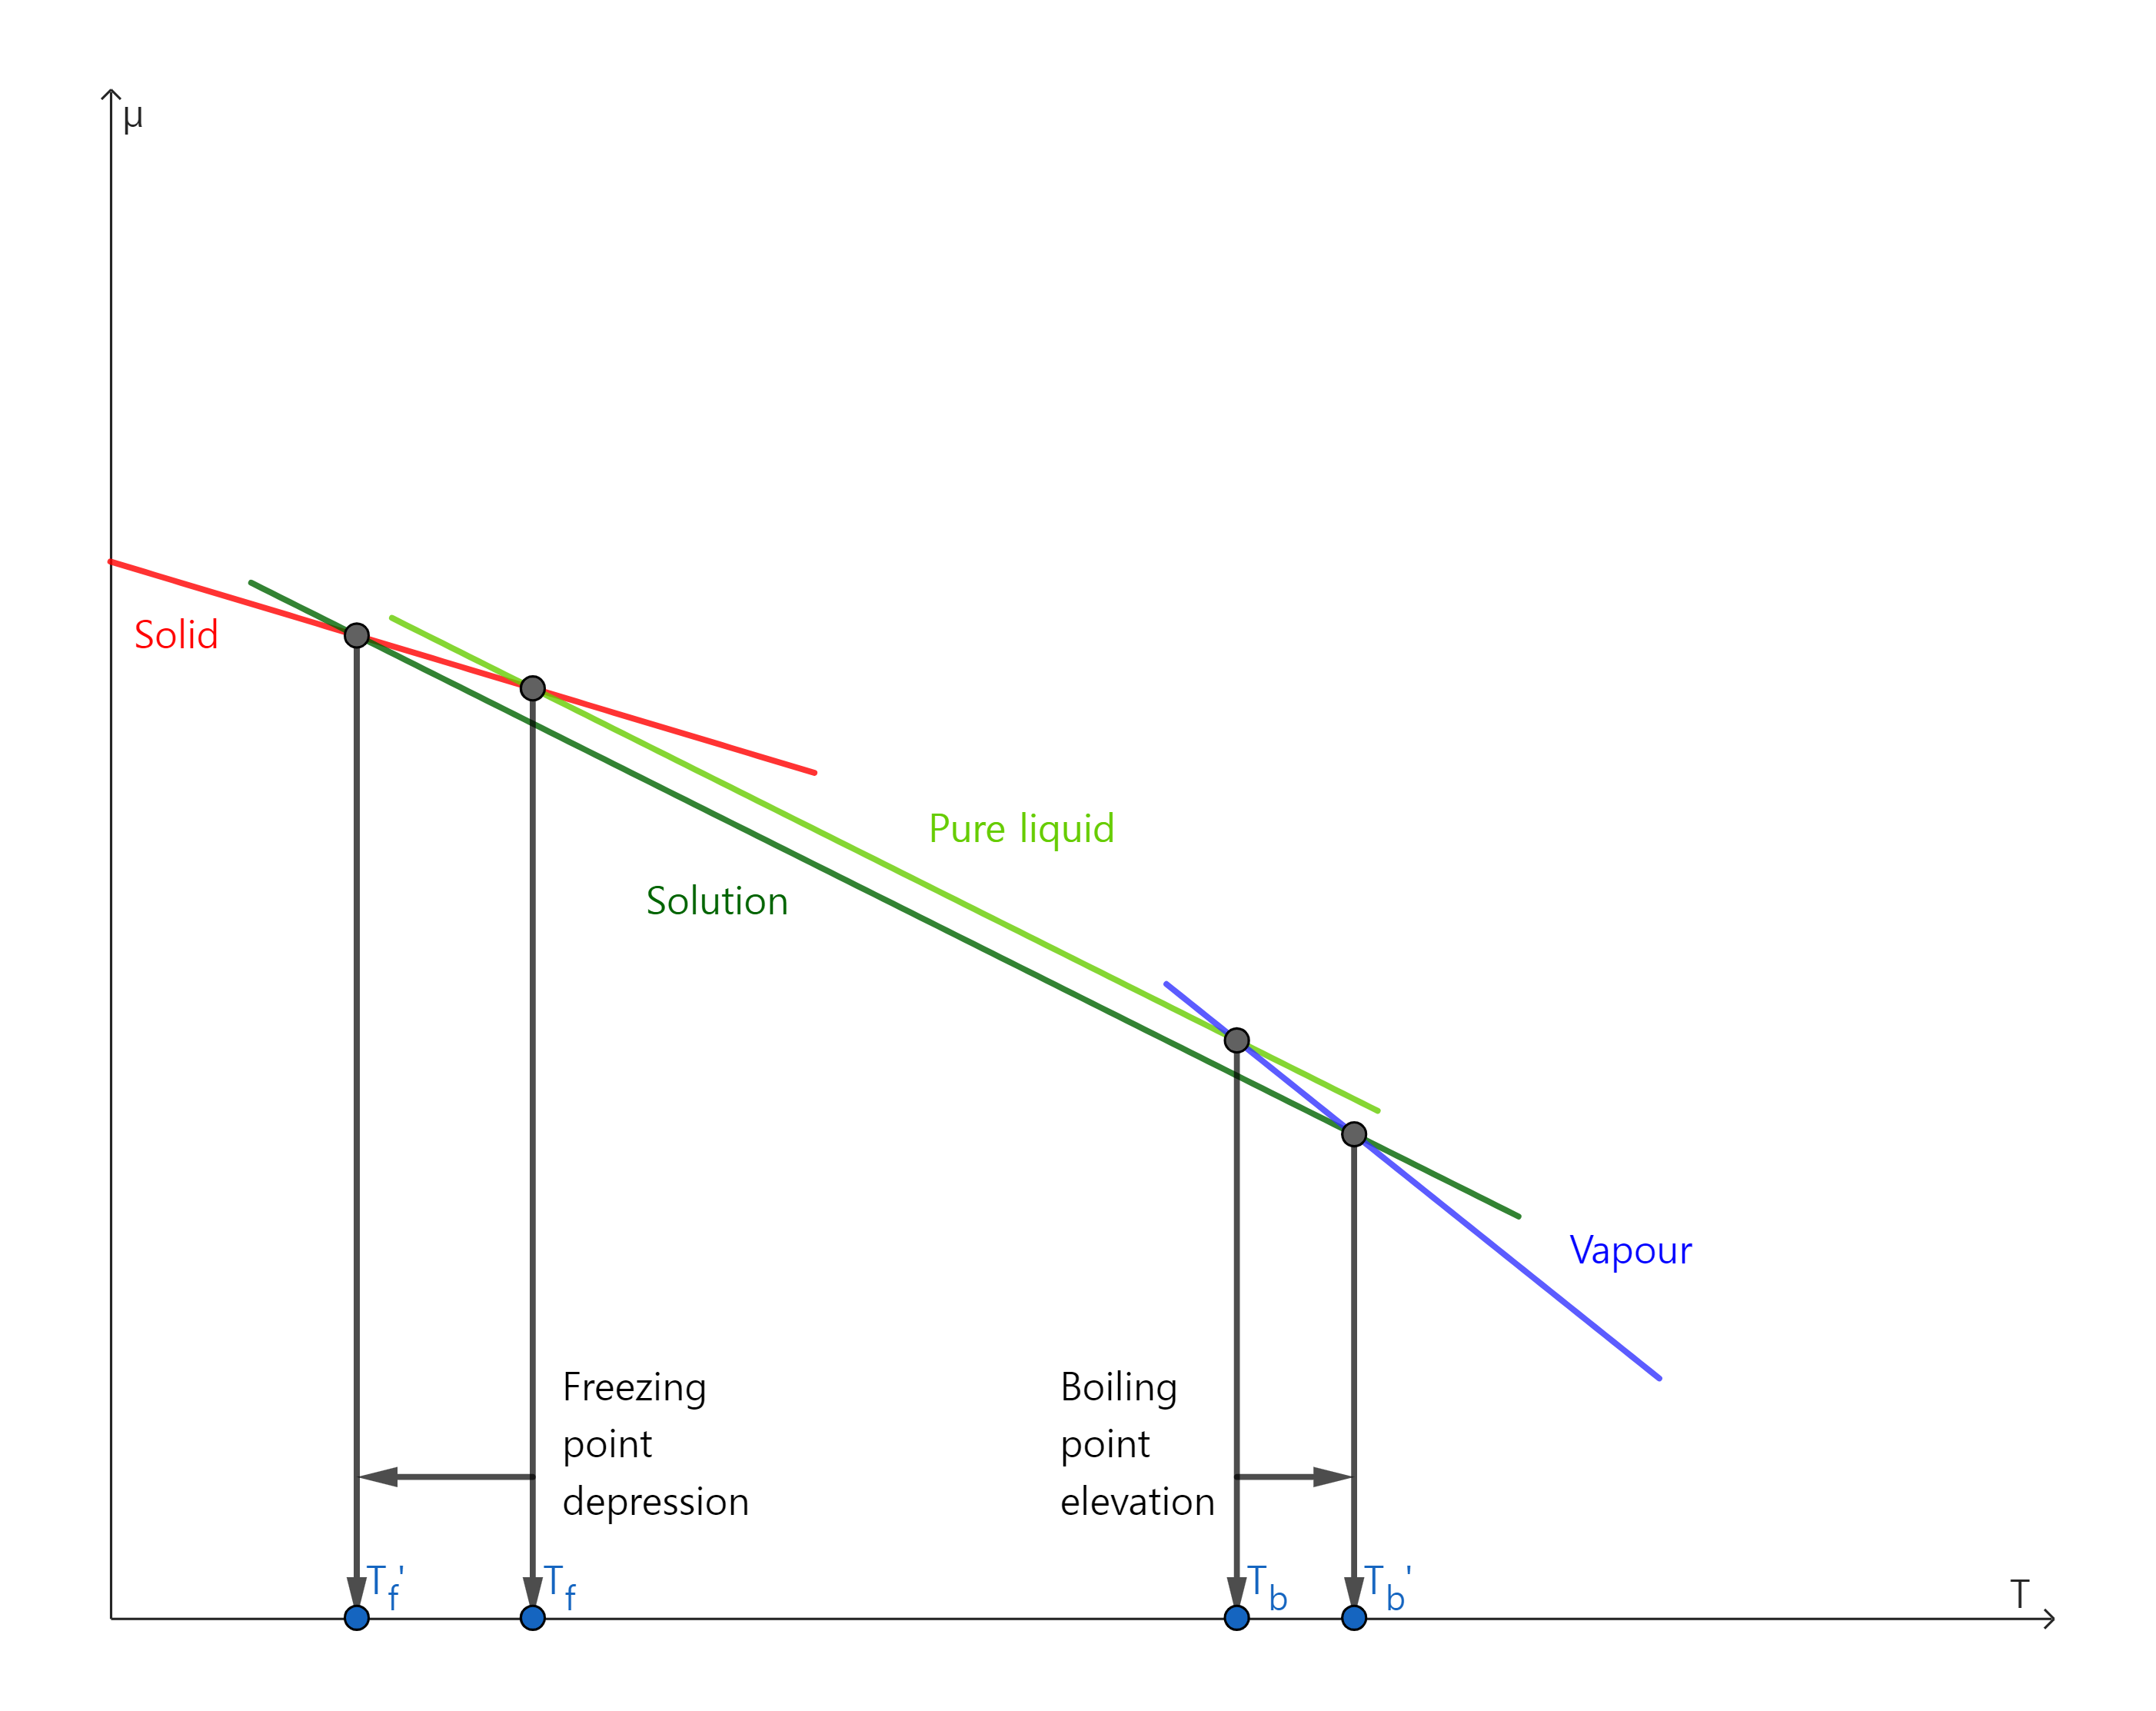
\includegraphics[scale=0.4]{Images/chempotcoll}
            \caption{상태 변화의 화학 퍼텐셜 변화}\label{f7}
        \end{figure}
        이는 이상 용액에서도 나타나는 현상이다. 따라서 이러한 현상은 엔트로피에 의한 것이다.
        \par 먼저 끓는점 오름을 유도해 보자.
        \begin{proof}[끓는점 오름]
        $\mu_A^\ast\left(\mathrm{g}\right)=\mu_A^\ast\left(\mathrm{l}\right)+RT\ln{x_A}$로부터 시작한다. 이때 
        별표는 순수한 물질에서의 상태를 나타낸다. 다시 정리하면 다음을 만족한다:
        $$
        \ln{x_A}=\frac{\mu_A^\ast\left(\mathrm{g}\right)-\mu_A^\ast\left(\mathrm{l}\right)}{RT}=\frac{\Delta_\mathrm{vap}G}{RT}
        $$
        이때 Gibbs-Helmholtz 방정식 (\ref{gheqn})을 이용해, 양변을 T로 미분하면
        $$
        \frac{\difform \ln{x_A}}{\difform T}=\frac{1}{R} \frac{\difform \left(\Delta_\mathrm{vap}G/T\right)}{\difform T}=-\frac{\Delta_\mathrm{vap}H}{RT^2}
        $$
        이 성립한다. 따라서 $\displaystyle\difform \ln{x_A}=-\frac{\Delta_\mathrm{vap}H}{RT^2}\difform T$에서, 
        양변을 적분하면 
        $$
        \int_{0}^{\ln{x_A}}\difform \ln{x_A^\prime}=-\frac{1}{R}\int_{T^\ast}{T}\frac{\Delta_\mathrm{vap}H}{T^{\prime 2}}\difform T^\prime
        $$
        이 성립한다. 이를 A와 B가 혼합된 이원계 혼합물에서 계산하면 다음과 같다:
        $$
        \ln{\left(1-x_B\right)}=\frac{\Delta_\mathrm{vap}H}{R}\left(\frac{1}{T}-\frac{1}{T^\ast}\right)
        $$
        $t <\!< 1$일 때 $\ln{\left(1-t\right)}\approx -t$로 근사할 수 있고, $T\approx T^\ast$에서 $\displaystyle\frac{1}{T^\ast}-\frac{1}{T}\approx \frac{T-T^\ast}{{T^\ast}^2} = \frac{\Delta T_b}{{T^\ast}^2}$이므로 
        다음이 성립한다:
        \begin{equation*}
            x_B = \frac{\Delta_\mathrm{vap}H}{R}\times\frac{\Delta T_b}{{T^\ast}^2}
        \end{equation*}
        이때 $K = \frac{R{T^\ast}^2}{\Delta_\mathrm{vap}H}$로 정의하면,
        \begin{equation*}
            \Delta T_b = K x_B
        \end{equation*}
        가 성립한다. 이를 \textbf{끓는점 오름(Elevation of boiling point)}이라 한다.
        \end{proof}
        \par 실제로는 경험적으로 몰랄 농도 $b$를 이용하여
        \begin{equation*}
            \Delta T_b = K_b b
        \end{equation*}
        를 쓴다. 이 $K_b$를 \textbf{끓는점 오름 상수(Boiling-point constant)}라 한다.
        \begin{proof}[어는점 내림]
        어는점 내림도 마찬가지로
        $$
        \mu_A^\ast\left(\mathrm{s}\right)=\mu_A^\ast\left(\mathrm{l}\right)+RT\ln{x_A}
        $$
        에서 출발하여 다음과 같은 식을 얻을 수 있다:
        \begin{equation*}
            \Delta T_f = K^\prime x_B
        \end{equation*}
        이때 $\displaystyle K^\prime = \frac{R{T^\ast}^2}{\Delta_\mathrm{fus}H}$이고, 이를 \textbf{어는점 내림(Freezing point depression)}이라 한다.
        \end{proof}
        \par 실제로는 경험적으로 몰랄 농도 $b$를 이용하여 
        \begin{equation*}
            \Delta T_f = K_f b
        \end{equation*}
        를 쓴다. 이 $K_f$를 \textbf{어는점 내림 상수(Freezing-point constant)}라 한다.
        \par 용해도의 경우에는 총괄성에 해당되지는 않지만(용질의 성질에 영향을 받으므로), 이상 용액은 열역학적으로 다음 식을 만족한다:
        \begin{equation*}
            \ln{x_B}=\frac{\Delta_\mathrm{fus}H}{R}\left(\frac{1}{T_f}-\frac{1}{T}\right)
        \end{equation*}
        \begin{defn}[삼투 현상과 삼투압]
        \textbf{삼투 현상(Osmosis)}은 서로 농도가 다른 두 용액이, 용매 분자는 통과시키지만 용질은 통과시키지 않는 \textbf{반투막(Semipermeable membrane)}을 사이에 
        두고 분리되어 있을 때 저농도에서 고농도로 용매가 흐르는 현상이다. \textbf{삼투압(Osmotic pressure, $\Pi$)}은 이때 용매의 흐름을 막기 위해 고농도 용액에 
        가해야 하는 압력이다.
        \end{defn}
        삼투 현상을 이용하여 거대 분자의 분자량을 측정할 수 있다. 이를 \textbf{삼투법(Osmometry)}이라 한다. 삼투 현상 또한 총괄성에 속한다. 
        \begin{proof}[삼투 현상]
        먼저 순수한 용매와 용액이 반투막으로 분리되어 있다고 하자. 평형 상태에서 다음 등식으로부터 출발한다:
        $$
        \mu_A^\ast\left(p\right)=\mu_A\left(x_A,p+\Pi\right)
        $$
        이때 $\mu_A\left(x_A,p+\Pi\right)=\mu_A^\ast\left(p+\Pi\right)+RT\ln{x_A}$를 만족하고, 이를 대입하면 다음이 성립한다:
        $$
        \mu_A^\ast\left(p+\Pi\right)=\mu_A^\ast\left(p\right)-RT\ln{x_A}
        $$
        식 \ref{gibbspartial}에 의해 $G_m\left(p_f\right)=G_m\left(p_i\right)+\int_{p_i}^{p_f}V_m \difform p$를 만족하므로, 다음을 
        만족한다:
        $$
        \mu_A^\ast \left(p+\Pi\right)=\mu_A^\ast\left(p\right) + \int_{p}^{p+\Pi}V_m \difform p
        $$
        위 식에서 $-RT \ln{x_A}=\int_{p}^{p+\Pi}V_m \difform p$을 만족하고, 용매의 몰 부피가 거의 일정하다고 가정하면 
        $\int_{p}^{p+\Pi}V_m\difform p = V_m \Pi$를 만족한다. 따라서
        $$
        -RT\ln{x_A}=V_m\Pi
        $$
        를 만족한다. 이때 $-RT\ln{x_A} = -RT\ln{\left(1-x_B\right)} \approx RTx_B$를 만족하므로, 묽은 용액의 삼투압은 다음과 같다:
        \begin{equation*}
            RTx_B=\Pi V_m
        \end{equation*}
        만약 B의 농도가 매우 묽을 경우, $x_B \approx n_B/n_A$로 근사할 수 있다. 따라서 $RT n_B \approx n_A \Pi V_m$을 만족하고, 
        $n_A V_m \approx V$이기 때문에 $RT n_B = \Pi V$, 즉 $V$를 양변에 나누면 다음과 같은 \textbf{van 't Hoff 방정식(van 't Hoff equation)}을 
        만족한다:
        \begin{equation*}
            \Pi = \left[ B \right]RT
        \end{equation*}
        이때 $\left[ J \right]$는 $J$의 몰 농도를 의미한다.
        \end{proof}
        여기서도 마찬가지로 비리얼 급수를 구할 수 있다 \textbf{(삼투 비리얼 급수(Osmotic virial expansion))}:
        $$
        \Pi = \left[ J\right]RT \left\{ 1+B\left[J\right]+\cdots\right\}
        $$
        이때 경험적인 계수 $B$는 \textbf{삼투 비리얼 계수(Osmotic virial coefficient)}라 한다.
    \section{이원계 상평형도: 액체}\label{ch5sub3}
        \hspace{\parindent}\textbf{증기 압력 그림(Vapour pressure diagram)}에서는 주어진 압력에서 평형을 이루는 분율을 나타낸 상평형도이다.
        두 휘발성 액체의 이상 용액에서, 부분 증기 압력은 Raoult 법칙에 의해 몰 분율과 비례한다:
        \begin{equation*}
            p_J = x_J p_J^\ast
        \end{equation*}
        따라서 혼합물의 총 증기 압력은 다음 Figure \ref{f8}을 따른다:\\
        \begin{figure}[H]
            \centering
            \begin{tikzpicture}
                \draw[black, thick, ->] (-3,-2.5) -- (-3,2.5) node[rotate = 90, midway, above] {압력, $p$};
                \draw[black, thick] (-3,-2.5) -- (3,-2.5) node[midway, below] {A의 몰 분율, $x_A$};
                \draw[black, thick, ->] (3,-2.5) -- (3,2.5);
                \draw[black, thick] (-3,-1.25) -- (3,1.5);
                \draw[black, thick, ->] (-2,-1.25) -- (-3,-1.25) node[midway, right=12pt] {$p_B^\ast$};
                \draw[black, thick, ->] (2,1.5) -- (3,1.5) node[midway, left=12pt] {$p_A^\ast$};
                \node at (-1,1.5) {Liquid};
                \node at (1,-1.5) {Vapour};
                \node[node font=\small, rotate=90, below right] at (-3,-2.5) {Pure B};
                \node[node font=\small, rotate=90, above right] at (3,-2.5) {Pure A};
                \node[below] at (-3,-2.5) {0};
                \node[below] at (3,-2.5) {1};
            \end{tikzpicture}
            \caption{Raoult 법칙을 만족할 때의 총 증기 압력}\label{f8}
        \end{figure}
        따라서 $p = p_A + p_B$를 따른다. 만약 증기에서의 몰 분율과 액체에서의 몰 분율이 다를 경우, 
        증기의 몰 분율 $y_J$를 다음과 같이 정의한다:
        \begin{equation*}
            y_J = \frac{p_J}{p}
        \end{equation*}
        만약 이상 용액일 경우, 액체의 몰 분율 $x_J$에 대해 다음을 만족한다:
        \begin{equation*}
            y_A = \frac{x_A p_A^\ast}{p_B^\ast + \left(p_A^\ast - p_B^\ast\right)x_A}
        \end{equation*}
        또한 $y_B = 1-y_A$를 만족한다. $p_A^\ast$와 $p_B^\ast$는 각 분자의 휘발성과 관련이 있고, 이 둘의 비율로 증기에 
        무엇이 더 많을지 예측할 수 있다. 즉 $p_A^\ast / p_B^\ast > 1$일 때, $y_A > x_A$를 만족한다.
        \par \textbf{온도-분율 그림(Temperature-composition diagram)}은 주어진 온도에서 평형 상태를 이루는 분율을 나타낸 상평형도이다. 
        이때, 압력은 주로 1 atm에서 측정한다. 이때 액체 상이 아래에 위치하고, 액체 상의 경계는 그 분율에서의 끓는점을 나타낸다. 또한 
        기체 상의 경계는 특정 온도에서 기체의 분율을 나타낸다. 그림은 다음 Figure \ref{f9}와 같다:\\
        \begin{figure}[H]
            \centering
            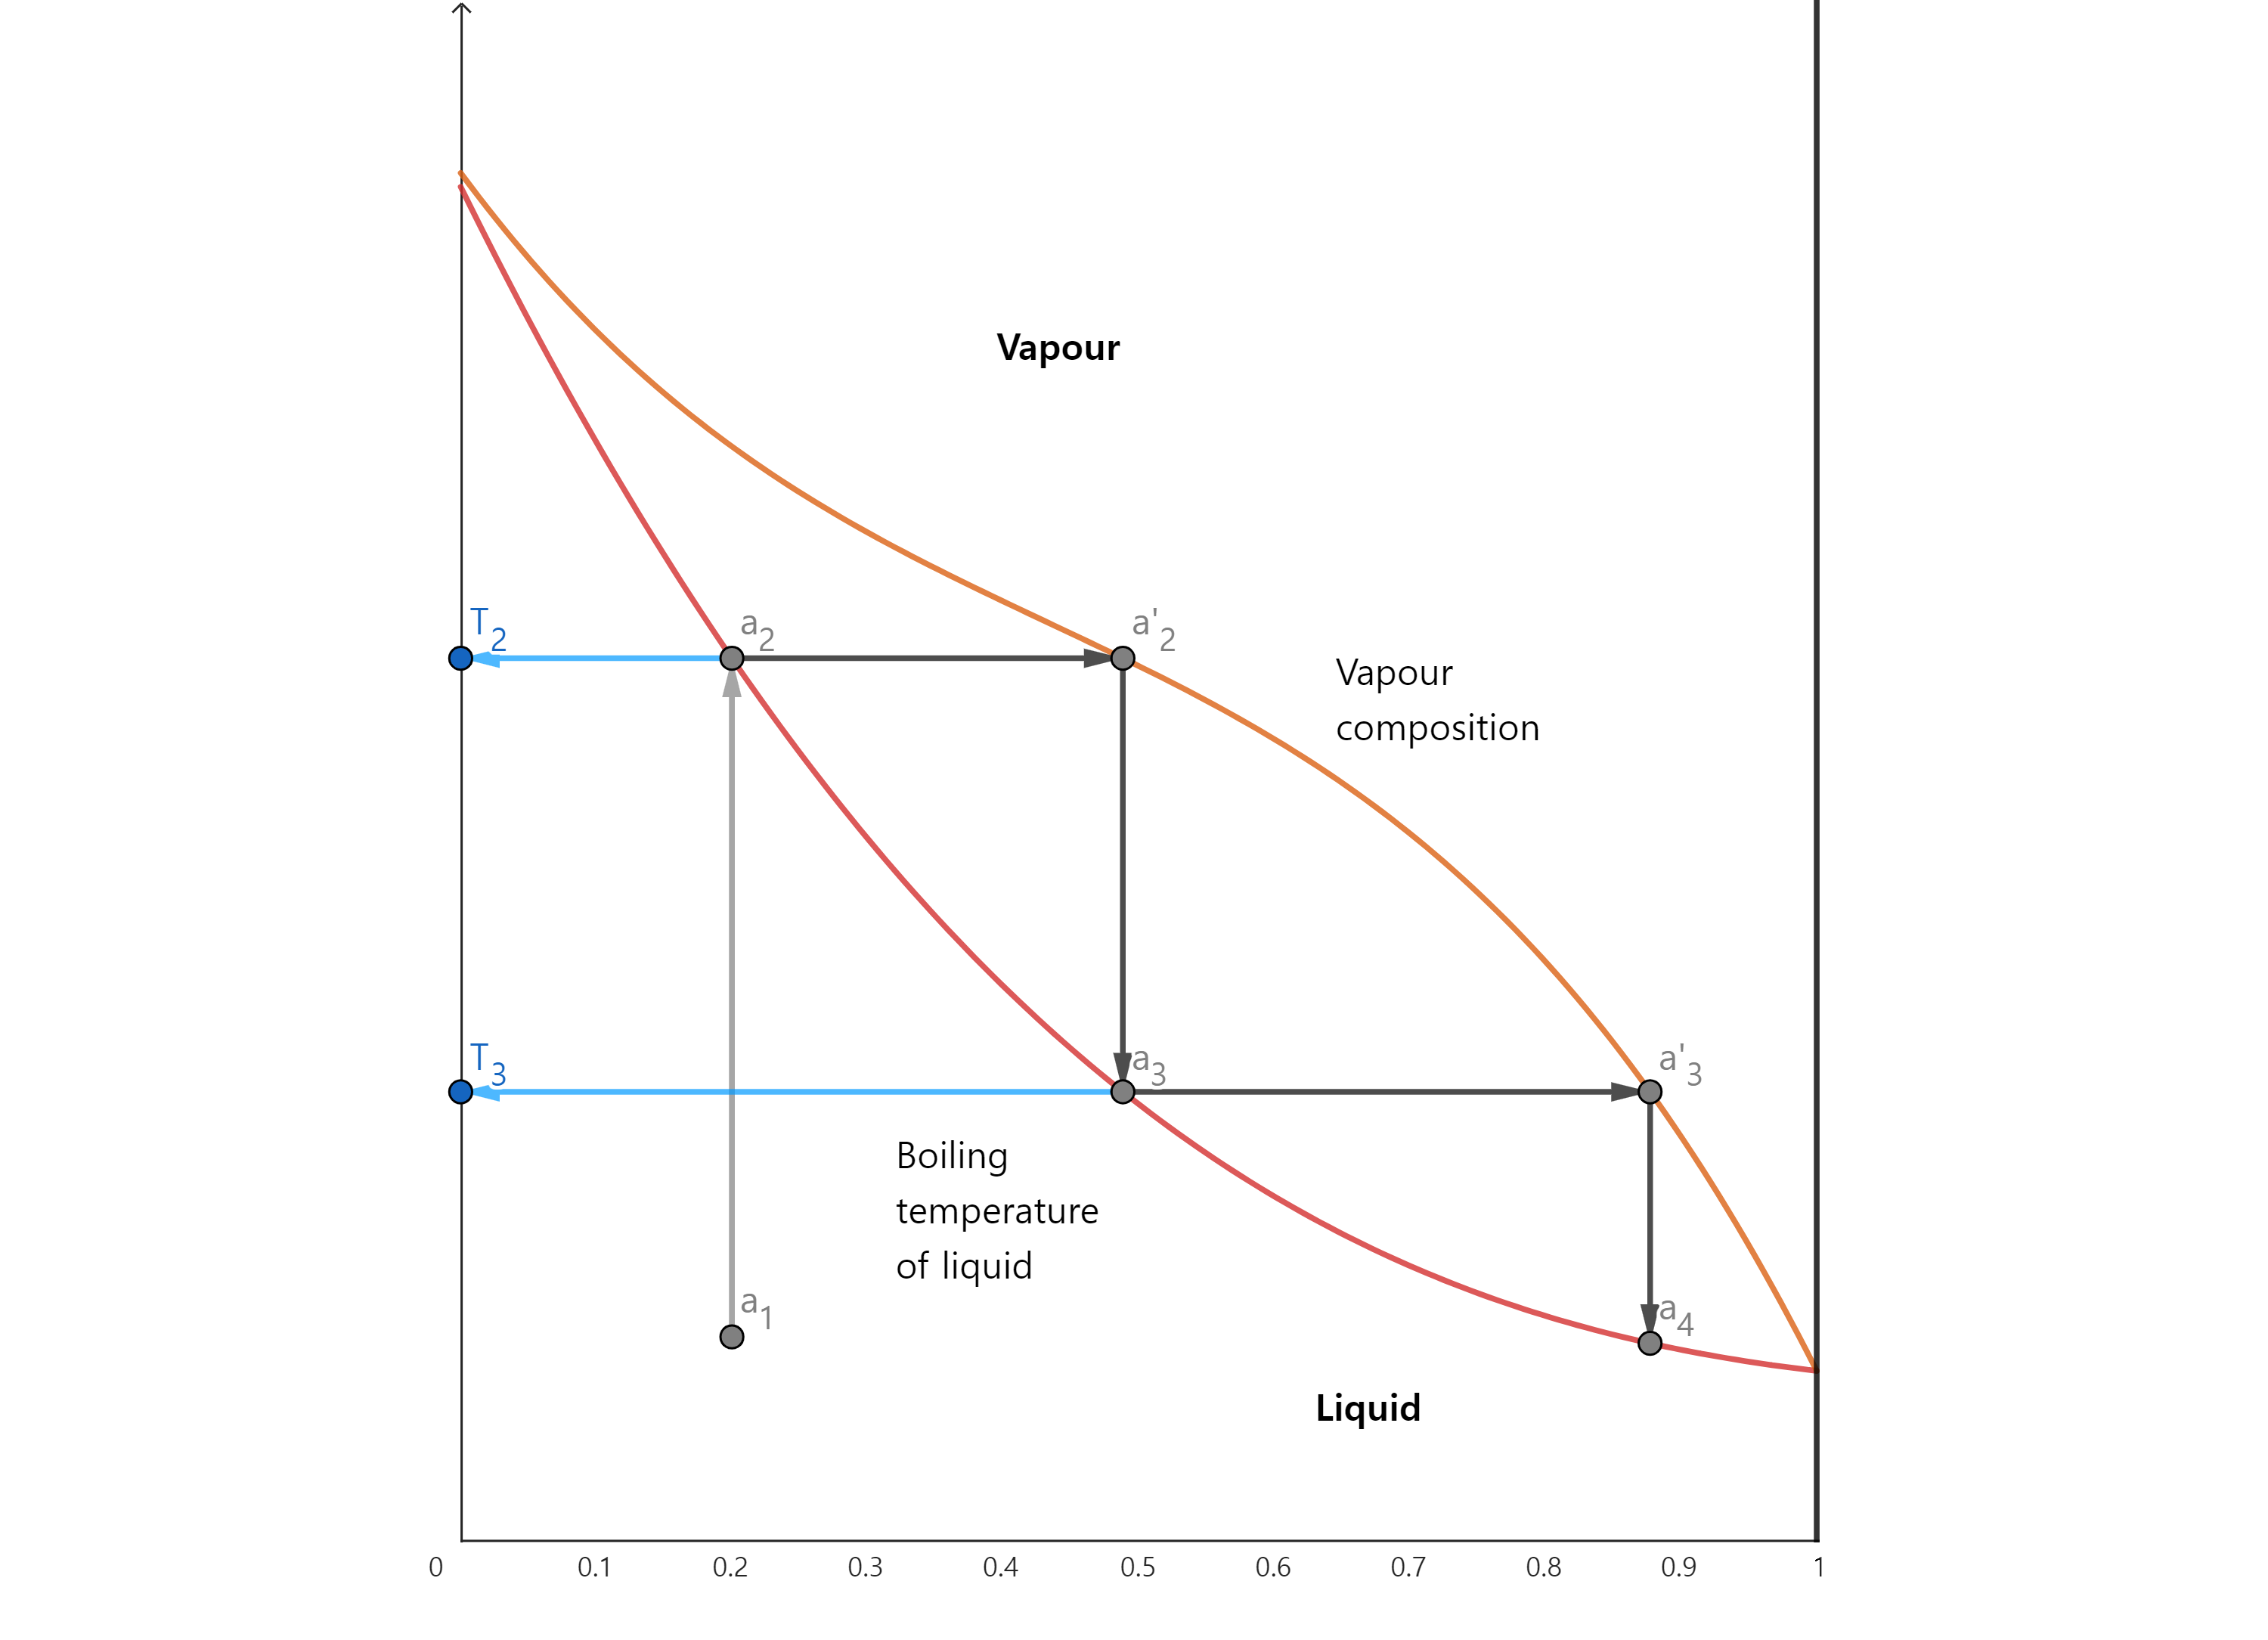
\includegraphics[scale=8]{Images/lgphasediag}
            \caption{온도-분율 그림}\label{f9}
        \end{figure}
        이는 증류 과정에서 중요하다. 즉, 같은 온도에서 기체를 응축하면 응축된 액체의 구성 분율은 달라진다. 이러한 그림에서 
        상 경계는 \textbf{공존 곡선(Coexistence curve)}이라고도 한다.
        \par 이제부터 지레 규칙에 대해 알아볼 것이다. 다음과 같은 Figure \ref{f10}을 생각하자:
        \begin{figure}[H]
            \centering
            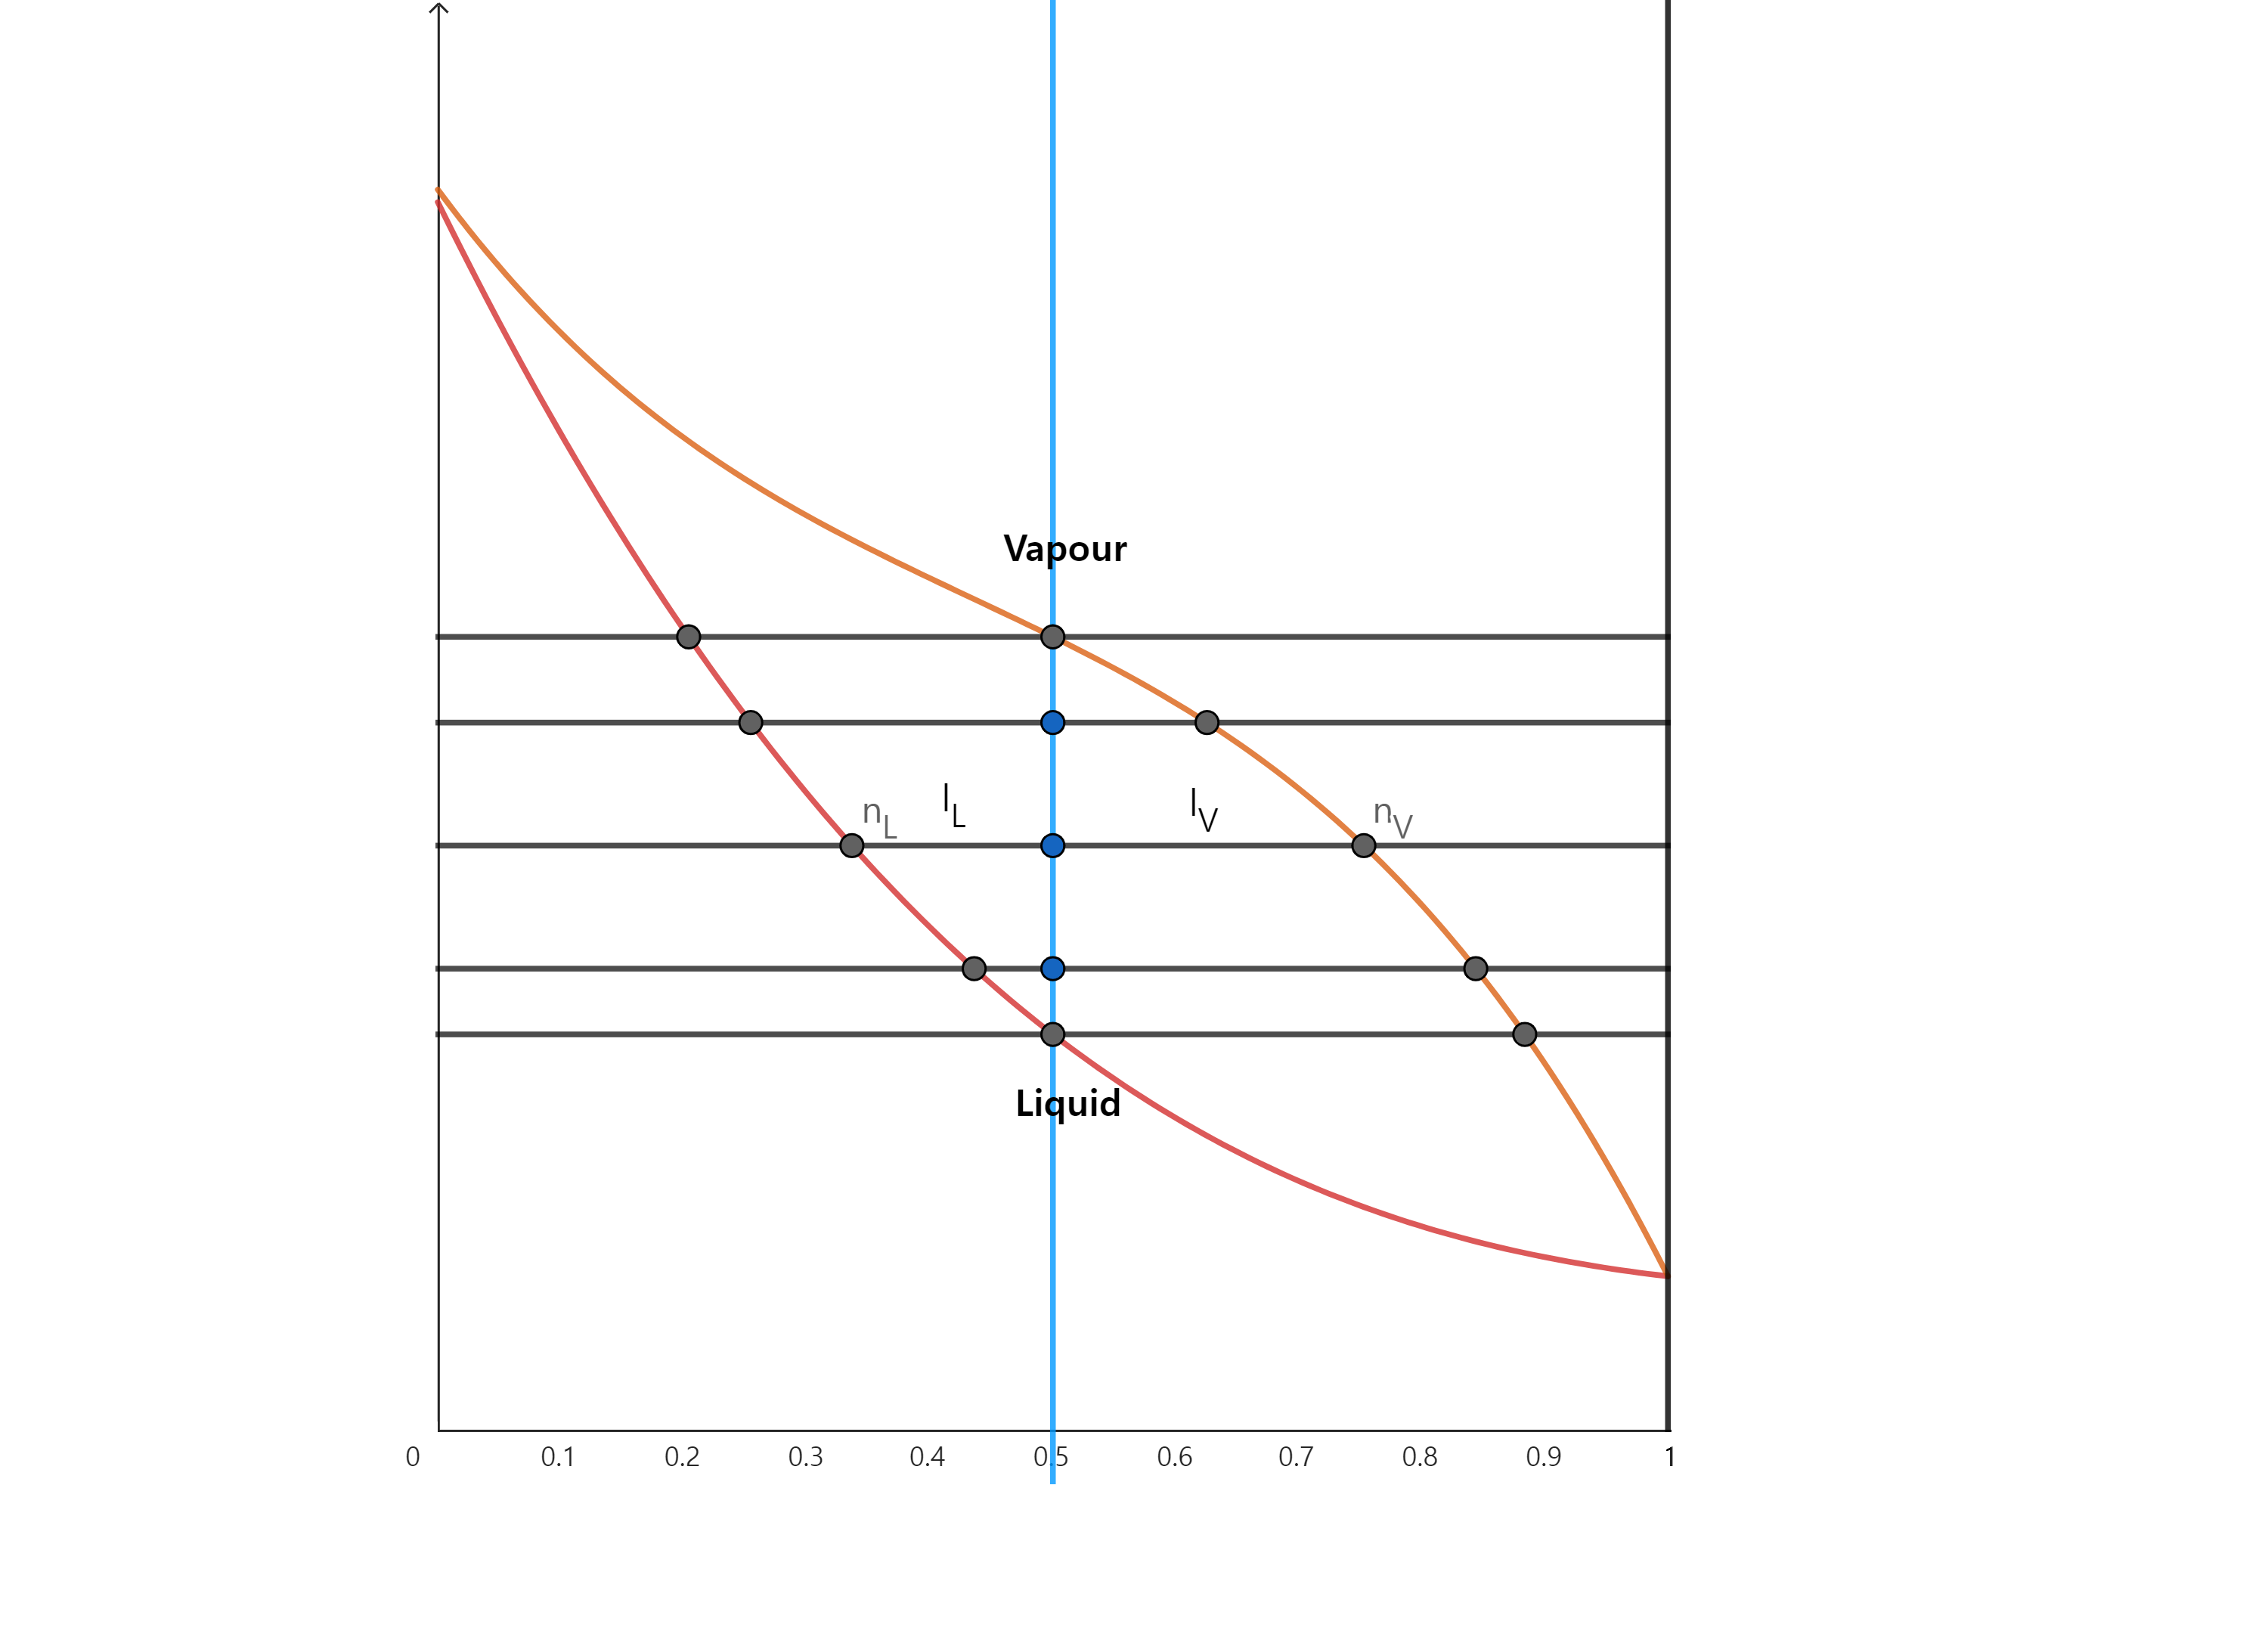
\includegraphics[scale=7]{Images/lgphasediaglever}
            \caption{온도-분율 그림에서의 지레 규칙}\label{f10}
        \end{figure}
        이때 구하고자 하는 몰 분율을 $z_A$라 하자. 이 온도에서 기체상은 $x_A$, 액체상은 $y_A$의 몰 분율을 가지고 있다고 하자. 이때 다음을 만족한다:
        \begin{equation*}
            n_A = n_L x_A + n_V y_A
        \end{equation*}
        또한 $z_A$에서 
        \begin{equation*}
            n_A = nz_A = n_L z_A + n_V z_A
        \end{equation*}
        를 만족한다. 이 둘을 연립하면 
        \begin{equation*}
            n_L\left(z_A - x_A\right) = n_V \left(y_A - z_A\right)
        \end{equation*}
        이때 주어진 점에서 각 공존 곡선까지의 '거리'를 다음과 같이 정의하자:
        \begin{align*}
        l_L &= z_A-x_A\\
        l_V &= y_A-z_A
        \end{align*}
        따라서 다음과 같은 \textbf{지레 규칙(Lever rule)}을 유도할 수 있다:
        \begin{law}[지레 규칙]
        \begin{equation*}
            n_L l_L = n_V l_V
        \end{equation*}
        \end{law}
        이러한 지레 규칙은 액체-기체 상평형도뿐만 아니라 모든 상평형도에서 성립한다. 또한, 일정한 몰 분율을 나타낸 직선을 \textbf{등치선(Isopleth)}이라 한다.
        \par \textbf{단순 증류(Simple distillation)}는 기화된 기체를 응축하여 분리하는 방법이다. 이는 비휘발성 고체나 용질로부터 휘발성 액체를 분리하는 데 이용한다. 
        또한 \textbf{분별 증류(Fractional distillation)}는 이러한 증류를 여러 번 하는 방법이다. 이때 분별 증류관의 효율은 
        \textbf{이론단수(Theoretical plates)}\footnote[13]{이 개념은 분석화학에서 크로마토그래피를 다룰 때에도 사용한다.}를 통해 나타낸다.
        \par 물과 에탄올의 혼합물과 같이, 증류 시 일정 지점을 기준으로 넘어갈 수 없는 경우가 존재한다. 이러한 경우를 \textbf{공비혼합물(Azeotrope)}이라 한다. 
        A-B 혼합물이 공비혼합물을 이룰 때, A-B 분자 간 상호작용이 액체를 안정화할 경우 초과 Gibbs 에너지 $G^E <0$을 만족한다. 따라서 증류 시 
        남아 있는 액체 혼합물의 분율이 일정 지점을 넘어갈 수 없다(High-boiling azeotrope). 또한, A-B 분자 간 상호작용이 액체를 불안정화할 경우, 
        초과 Gibbs 에너지 $G^E >0$을 만족한다. 따라서 증류 시 증기의 분율이 일정 지점을 넘어갈 수 없다(Low-boiling azeotrope). 다음 Figure \ref{f11}은 물-에탄올 혼합물의 
        온도-분율 그림이다\footnote[14]{https://www.science.smith.edu/~jbrady/petrology/igrocks-diagrams/binary/H2O-ethanol.php}:\\
        \begin{figure}[H]
            \centering
            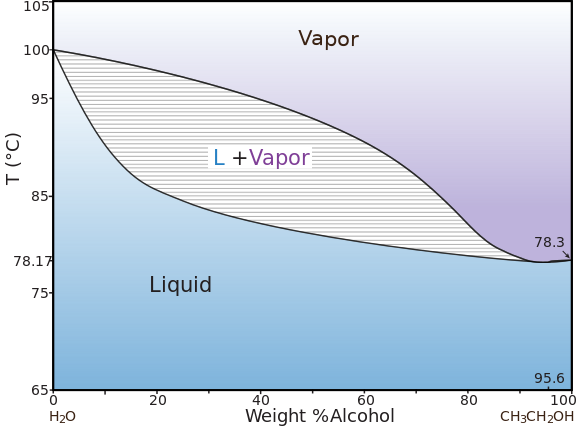
\includegraphics[scale=0.5]{Images/waterethanolazeo}
            \caption{물-에탄올 혼합물의 온도-분율 그림}\label{f11}
        \end{figure}
        이때 공비점인 에탄올 95.6 wt\%에서는 액체의 몰 분율과 기체의 몰 분율이 같아 더 이상 증류할 수 없다.
        \par 이제 섞이지 않는 두 액체에 대해 살펴보자. 서로 매우 적게 녹아있기 때문에, 총 증기 압력은 $p=p_A^\ast + p_B^\ast$에 가깝다. 
        만약 대기압과 총 증기 압력이 같아지면, 용액은 끓기 시작하고 용액에서 용해된 물질들이 분리되어 나온다. 
        대기압과 총 증기 압력이 같아지면 용액이 끓기 시작하는 성질을 이용한 증류를 \textbf{증기 증류(Steam distillation)}라고 한다. 
        이를 이용하면 열에 민감하고 물에 녹지 않는 유기물들을 끓는점보다 낮은 온도에서 분리할 수 있다. 만약 유기물의 휘발성이 낮다면, 
        증류가 어려울 수 있다.
        \par 액체-액체 상평형도는 \textbf{부분적으로 섞이는(Partially miscible)} 액체에 대해 적용할 수 있다. 일정 온도에서 일정 비율의 
        부분적으로 섞이는 액체 둘을 혼합하면 두 상으로 나뉜다. 즉 다음 Figure \ref{f12}와 같다:\\
        \begin{figure}[H]
            \centering
            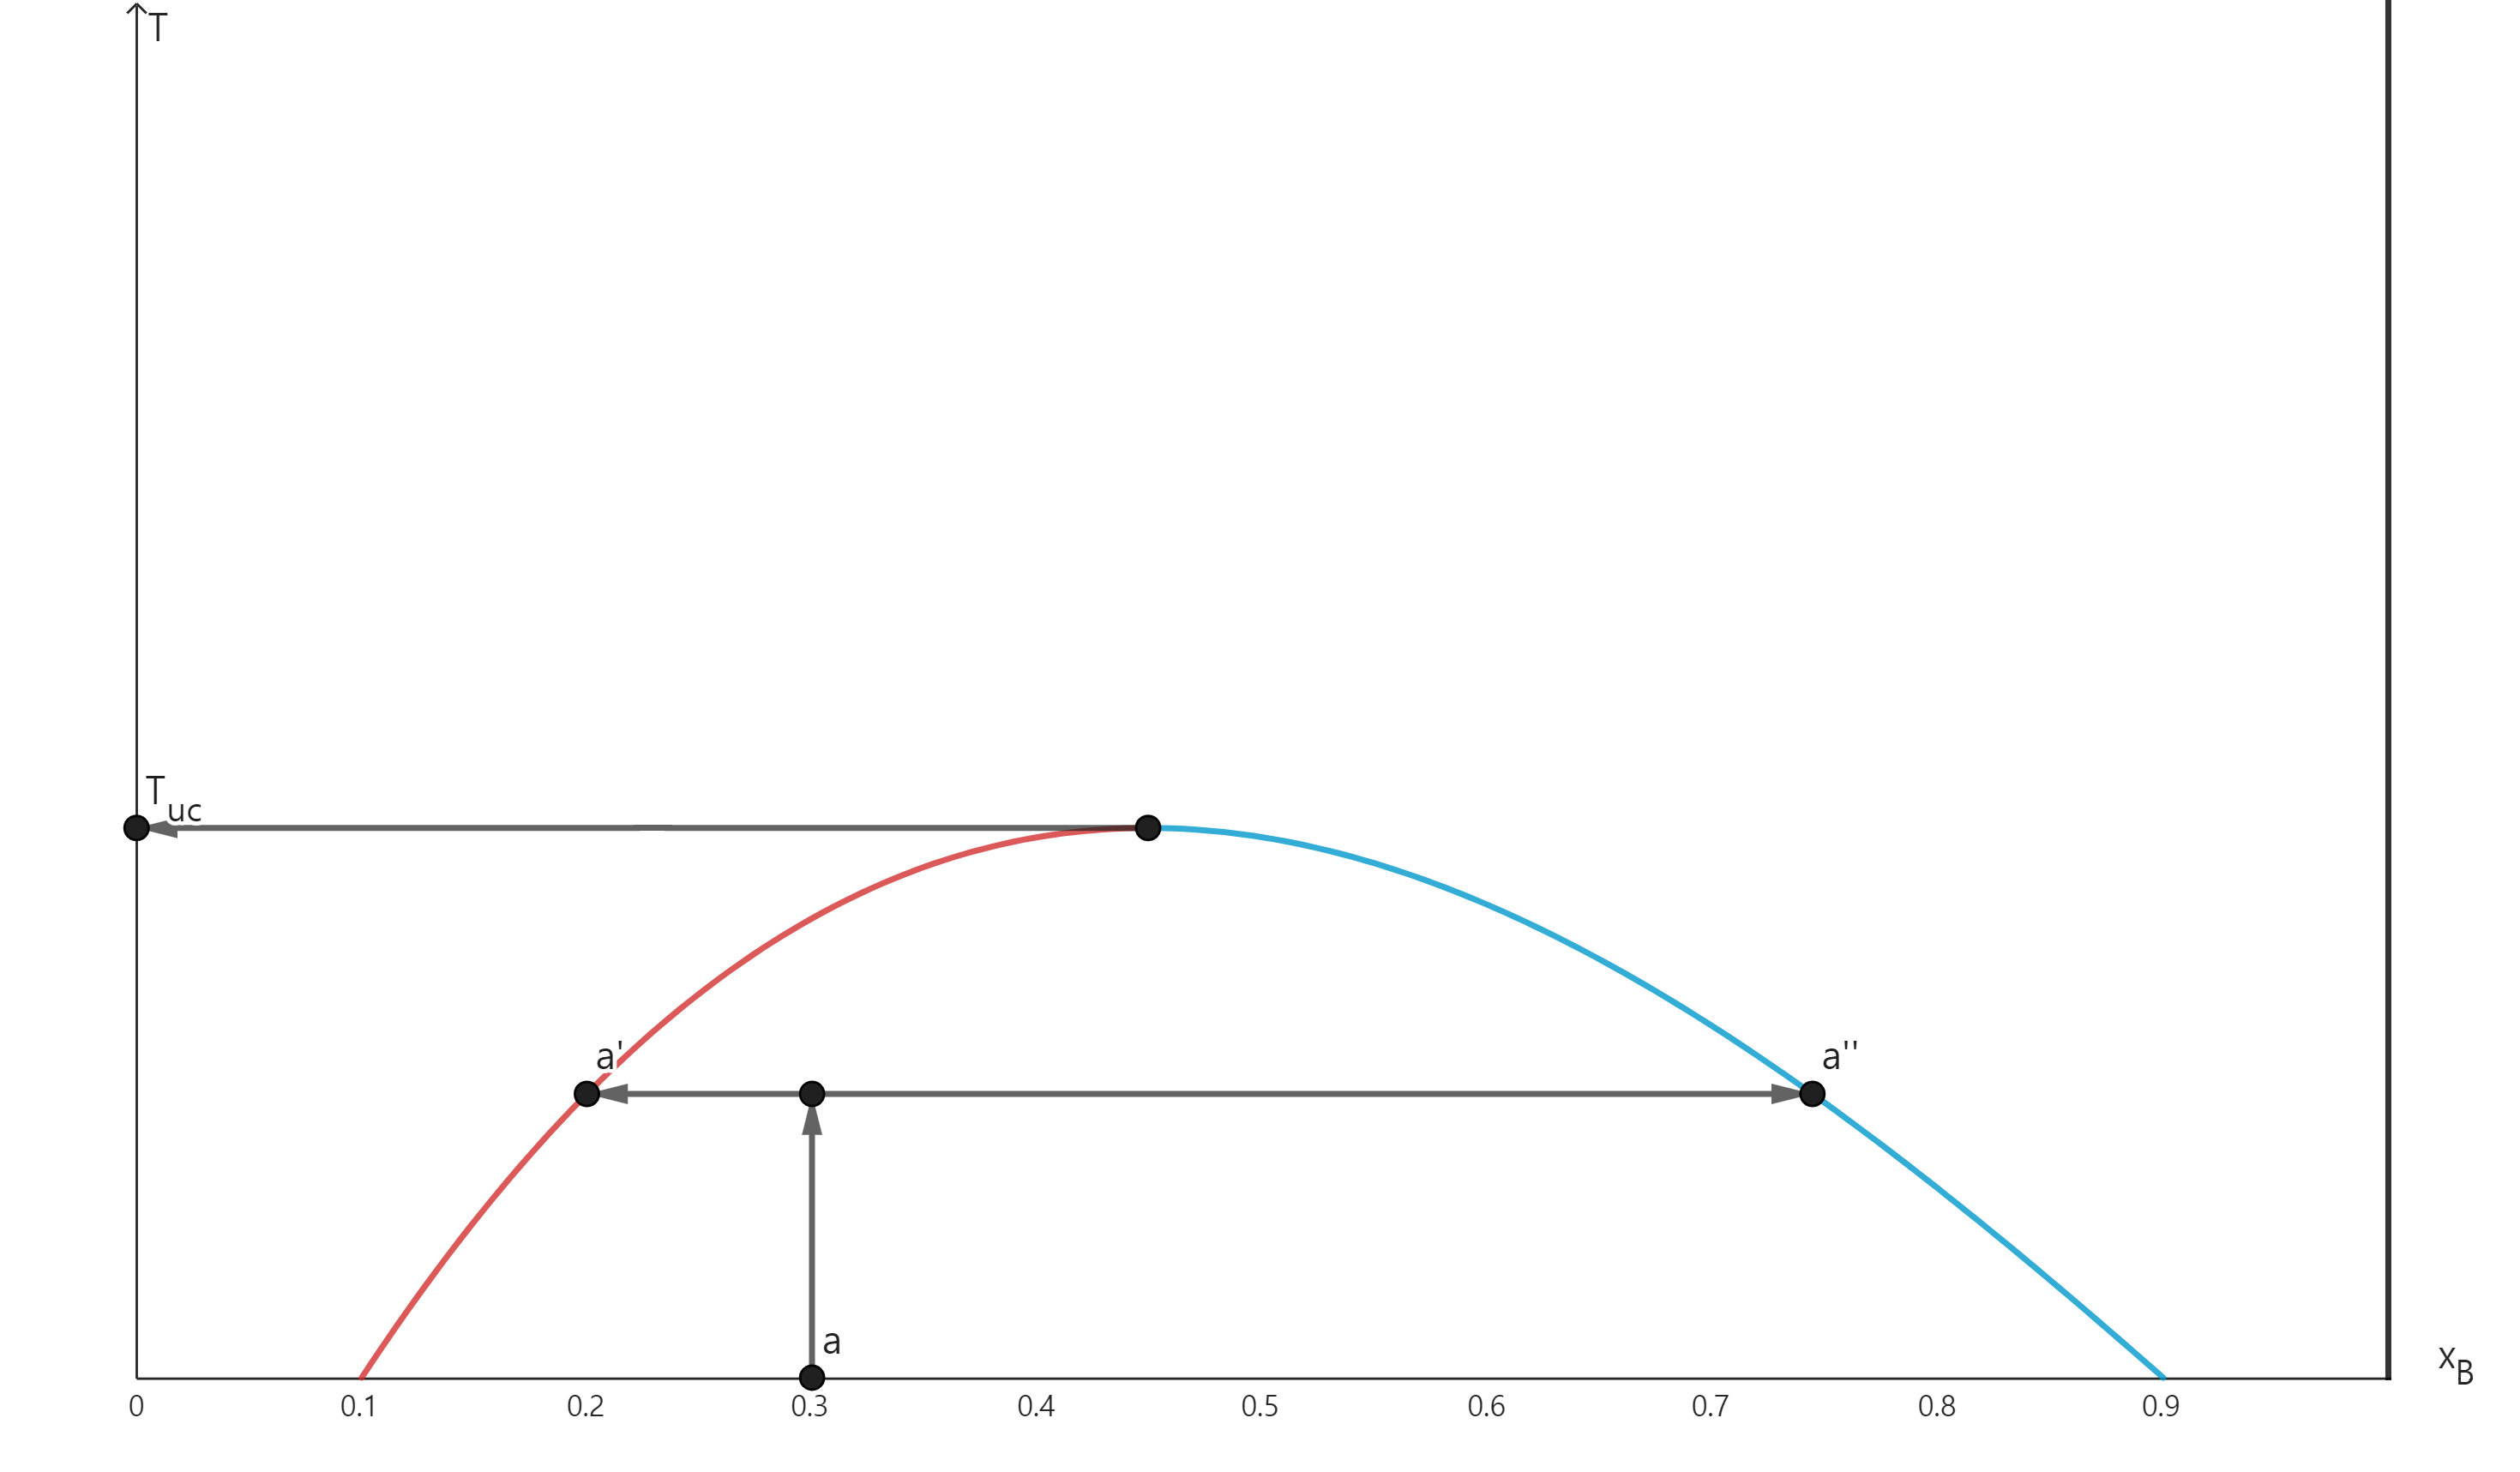
\includegraphics[scale=12]{Images/lldiaguc}
            \caption{액체-액체 상평형도}\label{f12}
        \end{figure}
        그림에서 나뉘는 부분은 $P=2$이고, 나뉘지 않는 부분은 $P=1$이다.
        \par 그림에서, $T_{uc}$ 이상의 온도에서는 어떤 분율을 취하더라도 완전히 섞인다. 이 온도를 
        \textbf{상부 임계 용해 온도(Upper critical solution temperature, UCST)}라 한다. 이 온도 이상에서는 분리되는 경우보다 
        섞이는 경우가 열역학적으로 유리하기 때문이다. 이를 열역학적으로 해석하자. 
        \par 식 \ref{excessenth}에서 도입한 $\xi$를 이용하자. $H^E = n\xi RTx_A x_B$이다. $\xi>2$일 때, 혼합 Gibbs 에너지는 극소점이 
        두 개 생긴다. 따라서 $\xi>2$일 때 상 분리가 발생한다. 이 최소점은 $\partial \Delta_\mathrm{mix}G/\partial x_A = 0$을 풀면 
        구할 수 있다. \ref{excessgibbs}로부터,
        \begin{equation*}
            \begin{aligned}
                &\left(\frac{\partial \Delta_\mathrm{mix}G}{\partial x_A}\right)_{T,p} \\
                &= nRT\left(\frac{\partial\left\{x_A\ln{x_A}+\left(1-x_A\right)\ln{\left(1-x_A\right)}+\xi x_A\left(1-x_A\right)\right\}}{\partial x_A}\right)_{T,p}\\
                &= nRT\left\{\ln{x_A}+1-\ln{\left(1-x_A\right)}-1+\xi\left(1-2x_A\right)\right\}\\
                &= nRT\left\{\ln{\frac{x_A}{1-x_A}}+\xi\left(1-2x_A\right)\right\}
            \end{aligned}
        \end{equation*}
        이므로 다음 방정식을 풀면 최소점을 구할 수 있다:
        \begin{equation*}
            \ln{\frac{x_A}{1-x_A}}=-\xi\left(1-2x_A\right)
        \end{equation*}
        이때 이 방정식은 해석적으로 풀 수 없으므로, 수치적으로 풀 경우 $\xi > 2$에서 상이 분리되는 것을 알 수 있다.
        \par 몇몇 계에서는 \textbf{하부 임계 용해 온도(Lower critical solution temperature, LCST; $T_{lc}$)}를 가진다. 
        이 경우 일정 온도 이하에서는 상이 분리되지 않으나, $T_\mathrm{lc}$ 이상에서는 상이 분리된다. 이는 저온에서 
        약한 복합체(complex)를 이루나, 그 이상의 온도에서 이러한 복합체가 분해되기 때문이다. 
        때에 따라 UCST와 LCST를 모두 가질 수 있다. 이는 낮은 온도에서는 약한 복합체를 이루고, LCST와 UCST 사이에서는 복합체가 분해된다. 
        이후 UCST 이상에서는 분자의 열운동이 혼합물의 상을 하나로 만든다. 이러한 혼합물의 예시는 니코틴과 물의 혼합물이 있다.
        \par 이러한 부분적으로 섞이는 용액을 증류할 때에도 상평형도를 이용할 수 있다. 
    \section{이원계 상평형도: 고체}
        \hspace{\parindent} 다음 Figure \ref{f13}과 같은 고체-액체 상평형도를 생각하자:\\
        \begin{figure}[H]
            \centering
            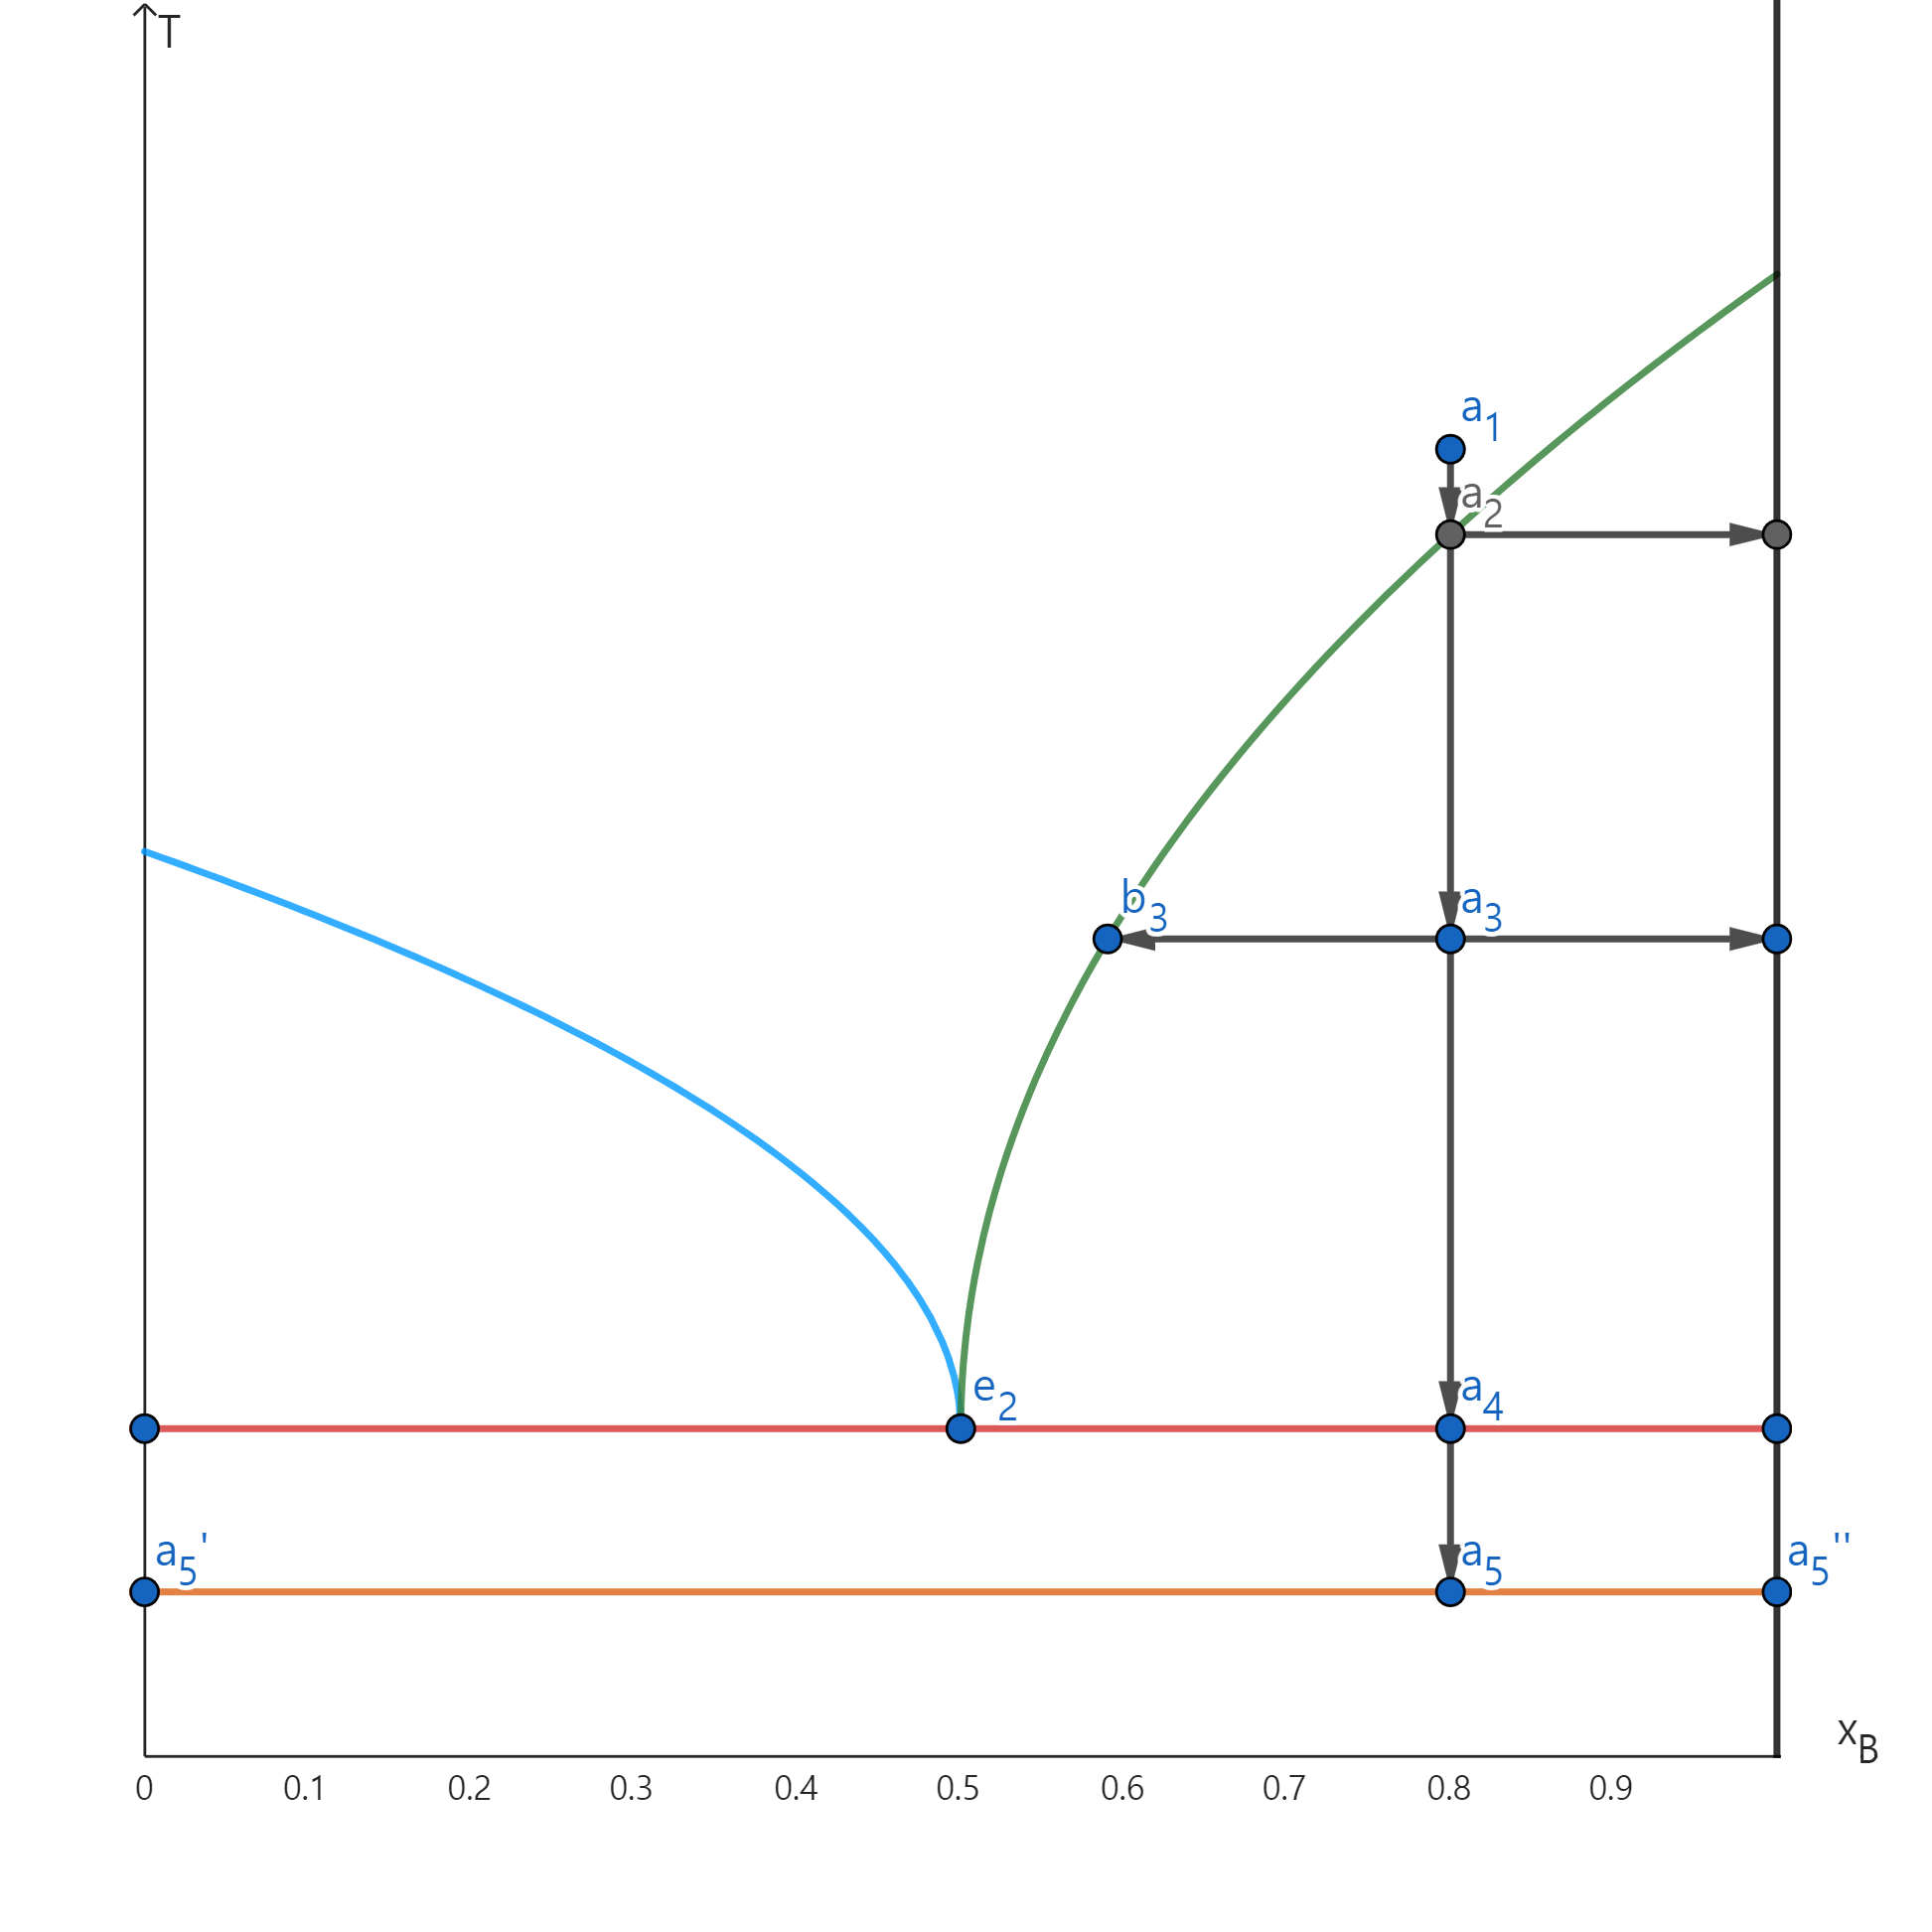
\includegraphics[width=0.7\linewidth]{Images/eutectic}
            \caption{고체-액체 상평형도}\label{f13}
        \end{figure}
        \par $a_1$에서 출발하자. $a_2$에 도달하면, B 고체가 생성되기 시작한다. $a_3$까지 온도를 내리면, 순수한 B 고체가 더 생성되고 $b_3$에 해당하는 액체가 남는다. 
        이제 $a_4$까지 내리자. 이제 액체의 분율은 $e_2$까지 내려간다. 이 이후로 온도가 더 내려가면 순수한 A 고체와 순수한 B 고체가 생성된다. 
        \par 이때 $e_2$ 점의 등치선은 \textbf{공정(Eutectic)}이라고 한다. 공정일 때 녹는점이 가장 낮고, 또한 이와 같은 분율일 때 액체를 냉각하면 순수한 A나 B가 만들어지지 
        않고 \textbf{판상(Lamellar)} 구조가 형성된다. 이러한 공정 상태를 알아내는 데에는 열 분석이 쓰일 수 있다. 특정 분율에서 등치선대로 온도를 내릴 때, 
        위의 Figure \ref{f13}에서 살펴보면 $a_1 \rightarrow a_2$에서 온도가 빠르게 하강하다가 $a_2 \rightarrow a_3$일 때 하강 속도가 느려지면서 순수한 B가 형성된다. 
        이후 $a_3 \rightarrow a_4$일 때 온도 변화가 없다. 이러한 온도 변화가 없는 지점을 \textbf{공정 중단(Eutectic halt)}이라고 한다.
        \par 다음과 같은, 화합물이 존재하는 상평형도(Figure \ref{f14})를 생각하자:\\
        \begin{figure}[H]
            \centering
            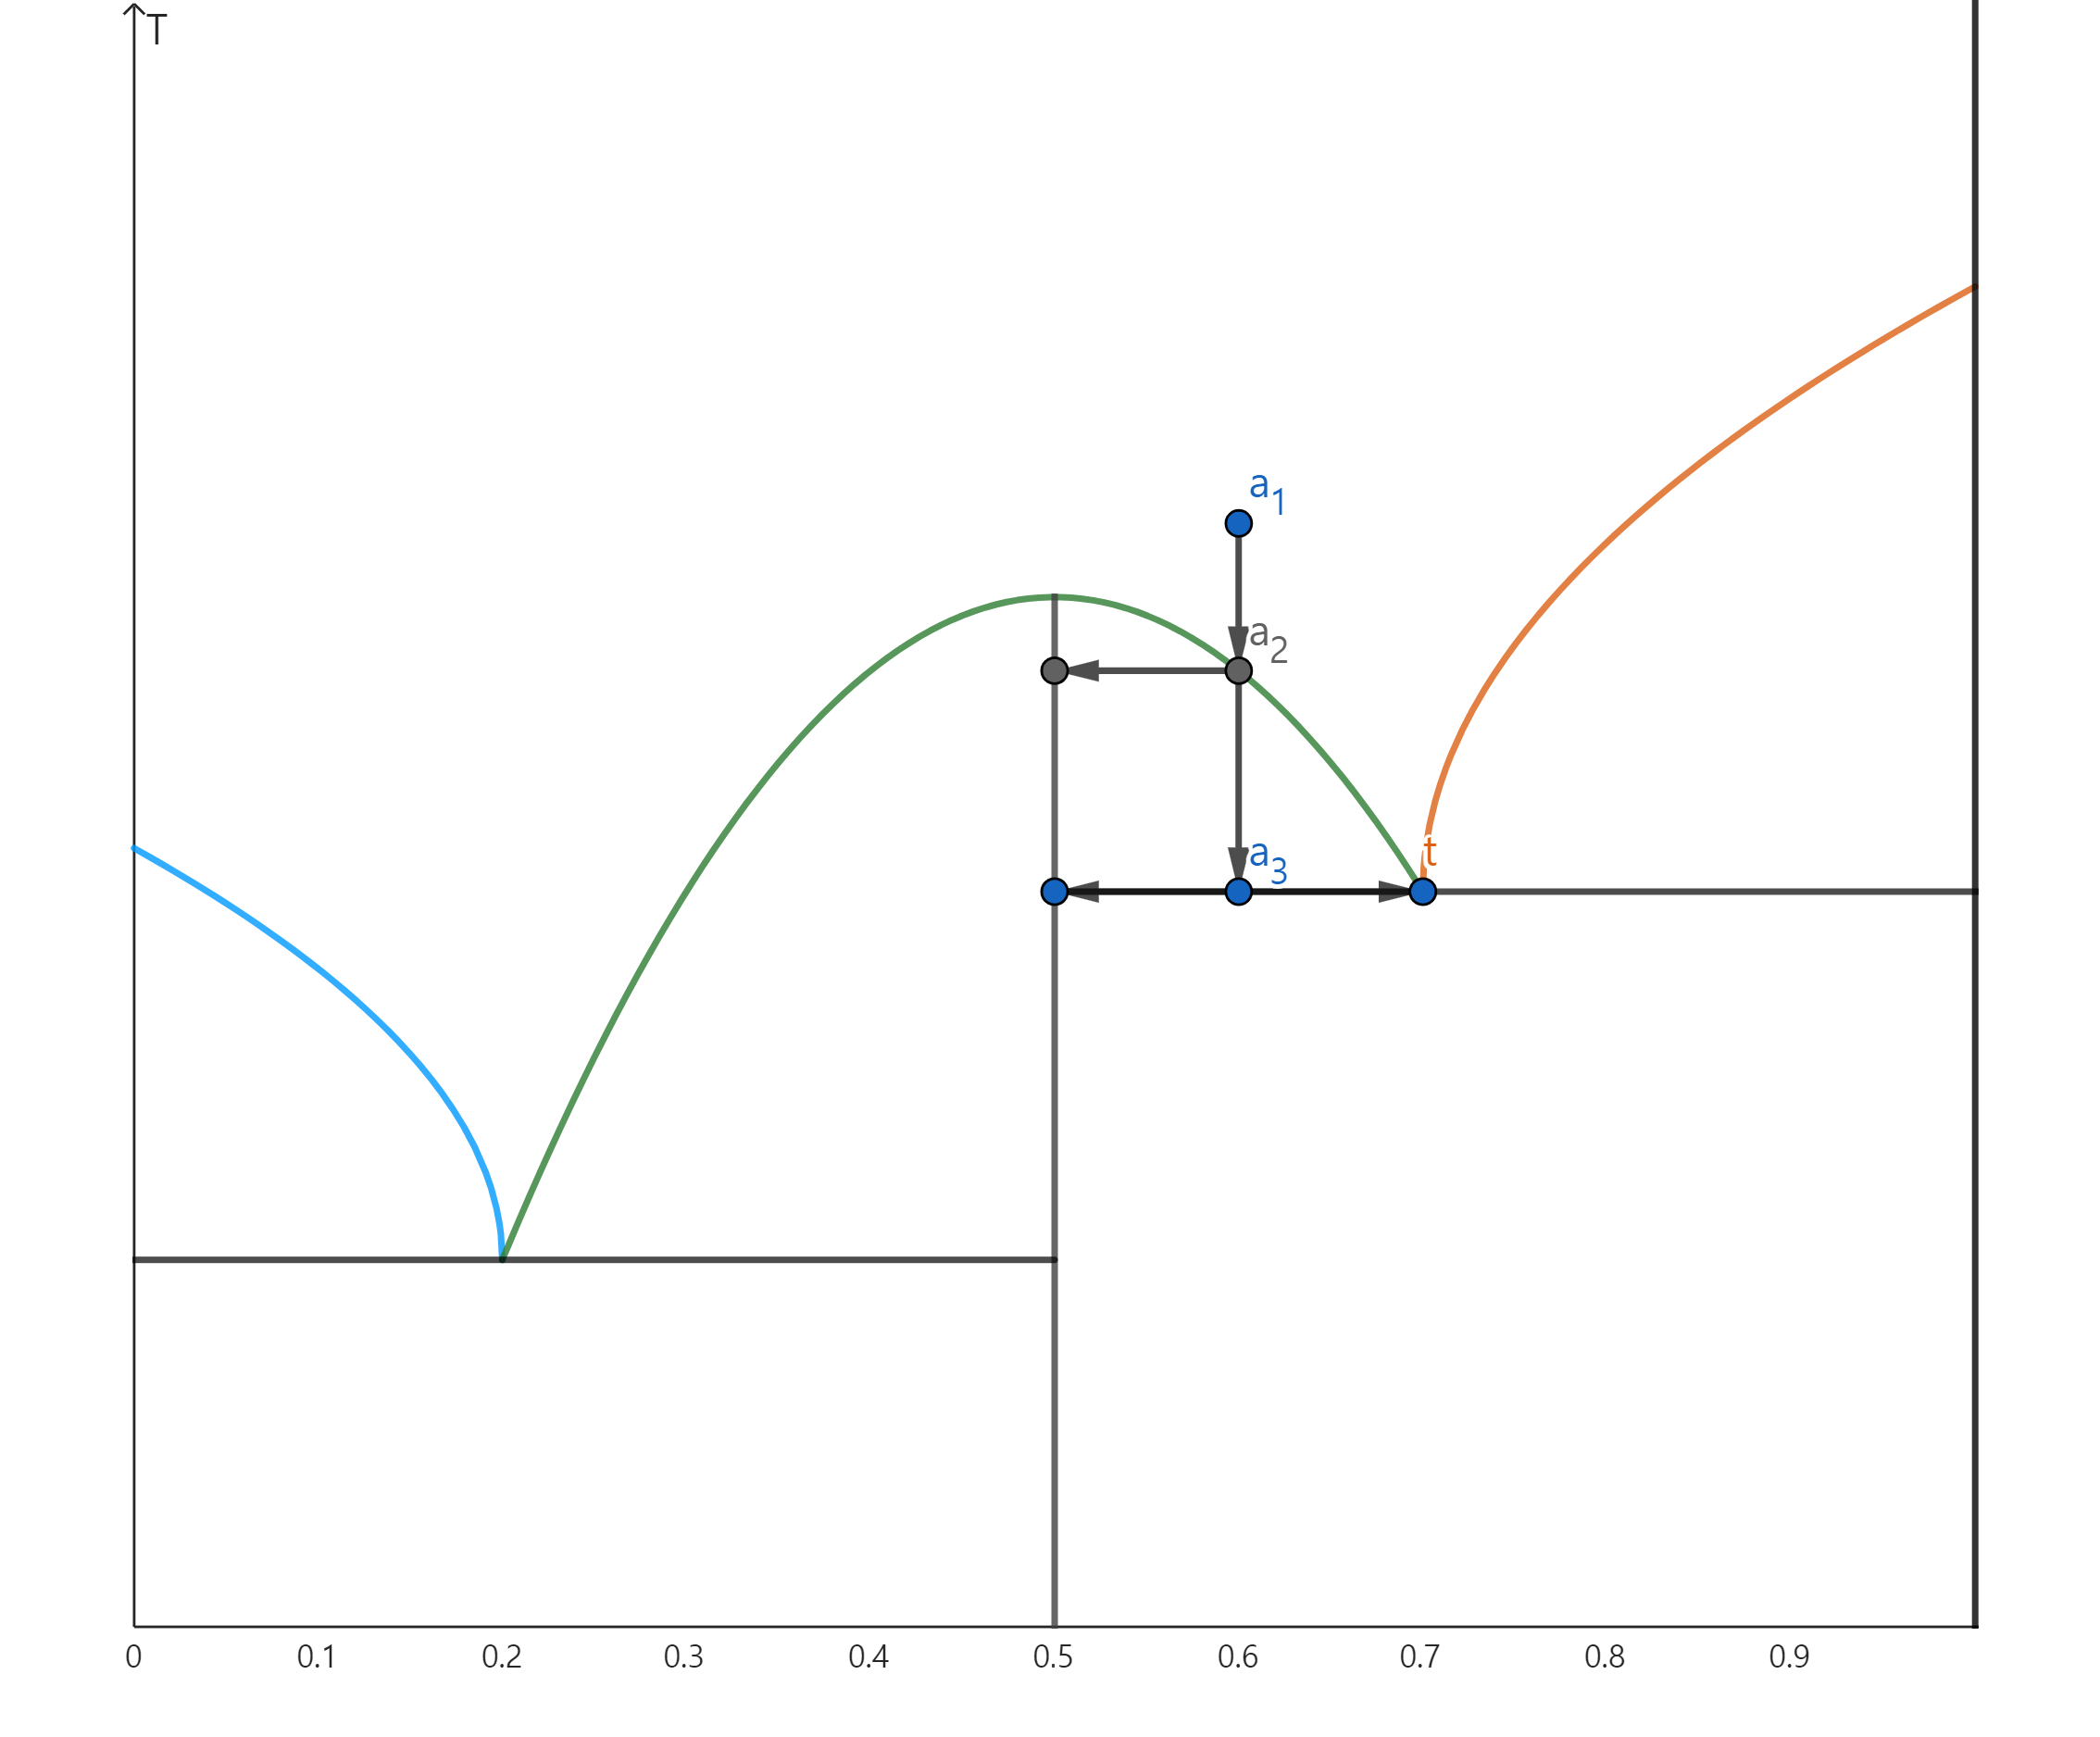
\includegraphics[scale=11]{Images/reactsys}
            \caption{화합물이 존재하는 고체-액체 상평형도}\label{f14}
        \end{figure}
        이 경우, 상평형도 여러 개로 쪼개어 생각할 수 있다. 즉, Figure \ref{f14}에서 왼쪽은 C, 오른쪽은 순수한 B가 존재하는 상평형도와, 왼쪽은 순수한 A, 오른쪽은 
        C가 존재하는 상평형도로 생각할 수 있다. (단, 가운데 화합물이 C라고 하자.) 이때 이 화합물 C는 이 분율을 유지하며 융해된다. 이를 \textbf{동질 용융(Congruent melting)}이라 
        한다. 그렇지 않은 경우를 \textbf{비동질 용융(Incongruent melting)}이라고 하는데, 이는 액체 화합물이 불안정하여 다른 상으로 분리되는 것을 의미한다.
    \section{삼원계 상평형도}
        \hspace{\parindent} 다음 Figure \ref{f15}와 같은 상평형도를 
        \textbf{삼원계 상평형도(Phase diagram of ternary system)}라 한다.
        \begin{figure}[H]
            \centering
            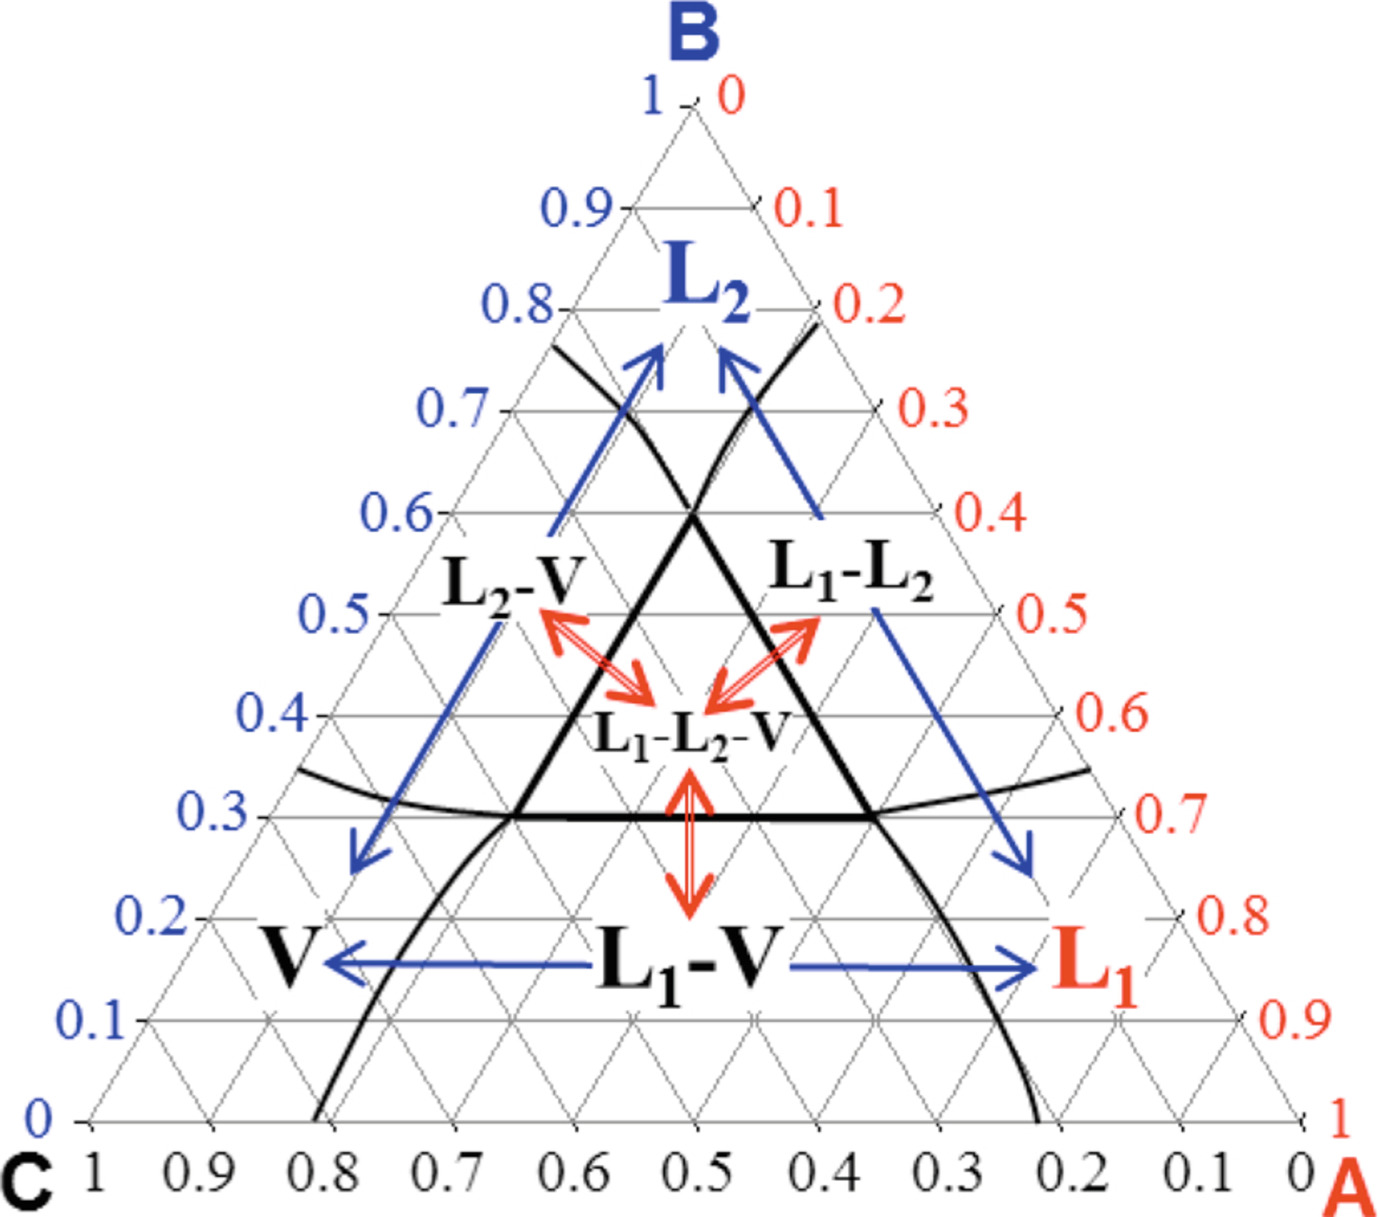
\includegraphics[width=0.6\textwidth]{Images/ternary}
            \caption{삼원계 상평형도}\label{f15}\cite{SMITH2013175}
        \end{figure}
        이때 밑변에서 1을 향하는 선에 수직인 선을 기준으로 성분의 분율을 읽어야 한다. 만약 삼원계 상평형도에서 서로 부분적으로 섞이는 쌍이 있을 경우, \ref{ch5sub3}에서의 논의를 마찬가지로 
        진행할 수 있다. 이러한 예시로는 물-아세트산-클로로폼의 혼합물로, 그 상평형도는 다음 Figure \ref{f16}과 같다. 
        \begin{figure}[H]
            \centering
            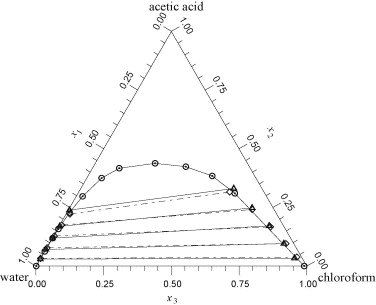
\includegraphics[width=0.6\textwidth]{Images/wtcternary}
            \caption{삼원계 상평형도}\label{f16}\cite{SENOL200651}
        \end{figure}
        이때 상이 분리되기 시작하는 지점을 \textbf{플레이트 포인트(Plait point)}라고 한다. 여기에서 상이 분리되는 두 점을 이은 선을 \textbf{대응선(Tie line)}이라 하고, 실험적으로 결정된다.
        고체에서도 마찬가지로 삼원계 상평형도를 결정할 수 있다.
    \section{활동도}
        \hspace{\parindent} 기체에서 화학 퍼텐셜은 $\mu_A = \mu_A^\ast + RT\ln{\left(p_A/p_A^\ast\right)}$와 같이 정의됨을 
        식 \ref{chempotgas}에서 살펴보았다. 이상 용액에서는 Raoult 법칙을 따르므로, $p_A = x_A p_A^\ast$가 성립한다는 사실에서 
        용액의 화학 퍼텐셜 $\mu_A = \mu_A^\ast +RT\ln{x_A}$가 성립한다. 실제 용액에서는 용질의 몰 분율 $x_A$ 대신 
        \textbf{활동도(Activity, $a_A$)}를 이용하여 다음과 같이 쓴다:
        \begin{equation*}
            \mu_A = \mu_A^\ast +RT\ln{a_A}
        \end{equation*}
        기체에서는 다음과 같이 정의된다:
        \begin{equation*}
            a_A = \frac{p_A}{p_A^\ast}
        \end{equation*}
        이러한 활동도는 '실효' 몰 분율로 볼 수 있다. 
        \par 모든 용매는 용질의 몰 분율이 0에 다가갈수록 Raoult 법칙을 따르므로, $a_A\rightarrow x_A$가 $x_A\rightarrow 1$일 때 성립한다. 
        이때 \textbf{활동도 계수(Activity coefficient, $\gamma_A$)}를 다음과 같이 정의한다:
        \begin{equation*}
            a_A = \gamma_A x_A
        \end{equation*}
        이때 $x_A\rightarrow 1$이면 $\gamma \rightarrow 1$이 모든 온도와 압력에서 성립한다. 따라서 화학 퍼텐셜은 다음과 같이 쓸 수 있다:
        \begin{equation*}
            \mu_A = \mu_A^\ast + RT\ln{x_A} + RT\ln{\gamma_A}
        \end{equation*}
        용매의 표준 상태는 $x_A=1$이고 압력이 $1$ bar일 때이다.
        \par Henry 법칙이 성립하는 이상 묽은 용액에서(즉, $x_B\rightarrow 0$), $p_B = K_B x_B$가 성립하므로 B의 화학 퍼텐셜은 
        \begin{equation*}
            \begin{aligned}
                \mu_B &= \mu_B^\ast +RT\ln{\frac{p_B}{p_B^\ast}} = \mu_B^\ast +RT \ln{\frac{K_B x_B}{p_B^\ast}}\\
                &= \mu_B^\ast +RT\ln{\frac{K_B}{p_B^\ast}}+RT\ln{x_B}
            \end{aligned}
        \end{equation*}
        이때 이상 묽은 용액에서 용질의 표준 화학 퍼텐셜을 다음과 같이 정의한다:
        \begin{defn}[이상 묽은 용액에서 용질의 표준 화학 퍼텐셜]
        \begin{equation*}
            \mu_B^\circlehbar = \mu_B^\ast +RT\ln{\frac{K_B}{p_B^\ast}}
        \end{equation*}
        \end{defn}
        따라서 이상 묽은 용액의 화학 퍼텐셜은 다음과 같이 다시 쓸 수 있다:
        \begin{equation*}
            \mu_B = \mu_B^\circlehbar + RT\ln{x_B}
        \end{equation*}
        만약 용액이 이상적이면, $K_B = p_B^\ast$이고 이는 Raoult 법칙에 해당한다. 따라서 이때 $\mu_B^\circlehbar = \mu_B^\ast$가 
        성립한다.
        \par 실제 용액에서는 다음과 같이 거동한다:
        \begin{equation*}
            \mu_B = \mu_B^\circlehbar + RT\ln{a_B}
        \end{equation*}
        이상 용액에서의 식과 실제 용액에서의 식을 각각 전개하여 합치면, 
        \begin{equation*}
            \begin{aligned}
                \mu_B &= \mu_B^\circlehbar - RT\ln{\frac{K_B}{p_B^\ast}} + RT \ln{\frac{p_B}{p_B^\ast}} \\
                &= \mu_B^\ast + RT\ln{\frac{p_B}{K_B}}
            \end{aligned}
        \end{equation*}
        과 같다. 따라서 활동도를 다음과 같이 정의할 수 있다:
        \begin{defn}[실제 용액에서의 용질의 활동도]
        \begin{equation*}
            a_B = \frac{p_B}{K_B}
        \end{equation*}
        \end{defn}
        마찬가지로 활동도 계수 또한 다음과 같이 정의된다:
        \begin{equation*}
            a_B = \gamma_B x_B
        \end{equation*}
        만약 $x_B \rightarrow 0$일 때 이상 묽은 용액의 거동을 따르므로, 이 경우 $a_B \rightarrow x_B$와 $\gamma_B \rightarrow 1$이 
        모든 온도와 압력에서 성립한다.
        \par 몰 분율 대신 몰랄 농도를 이용하여 다시 정의할 수 있다. 몰랄 농도를 $b$로 나타내면, 다음이 성립한다:
        \begin{equation*}
            \mu_B = \mu_B^\circlehbar +RT \ln{\frac{b_B}{b^\circlehbar}}
        \end{equation*}
        이때의 $\mu_B^\circlehbar$은 몰 분율을 이용할 때의 $\mu_B^\circlehbar$과 다른 값이다. 즉 $b = b^\circlehbar$일 때의 화학 퍼텐셜이다.
        이때 $b_B\rightarrow 0$일 때, $\mu_B \rightarrow -\infty$이다. 이는, 용액을 무한히 묽히면 용액이 무한히 안정해짐을 나타낸다. 
        실제 상황에 대입하면, 용액을 완벽히 분리하는 것이 매우 어려움을 나타낸다. 이때 실제 용액의 활동도 (계수)는 다음과 같이 정의한다:
        \begin{equation*}
            a_B = \gamma_B \frac{b_B}{b^\circlehbar}
        \end{equation*}
        이때 $b_B \rightarrow 0$일 때 $\gamma_B \rightarrow 1$이 성립한다. 따라서 실제 용액에서도 몰랄 농도를 이용해 다음과 같이 쓸 수 있다:
        \begin{equation*}
            \mu_B = \mu_B^\circlehbar + RT\ln{a_B}
        \end{equation*}
        \par 정규 용액에서는, 식 \ref{reggibbs}에서 출발한다. 이상 용액의 \\
        $$
        \Delta_\mathrm{mix}G = nRT\left\{x_A\ln{x_A} + x_B\ln{x_B}\right\}
        $$
        에서, 이상 용액이 아닐 경우에는 식이 다음과 같이 변화한다:
        \begin{equation*}
            \Delta_\mathrm{mix}G = nRT\left\{x_A\ln{a_A} + x_B\ln{a_B}\right\}
        \end{equation*}
        활동도 계수 표현으로 바꾸면 다음과 같다:
        \begin{equation*}
            \begin{aligned}
                \Delta_\mathrm{mix}G &= nRT\left\{x_A\ln{x_A\gamma_A}+x_B\ln{x_B\gamma_B}\right\}\\
                &= nRT\left\{x_A\ln{x_A} + x_B\ln{x_B}+x_A\ln{\gamma_A}+x_B\ln{\gamma_B}\right\}
            \end{aligned}
        \end{equation*}
        두 식을 합치기 위해 $\ln{\gamma_A} = \xi {x_B}^2$와 $\ln{\gamma_B} = \xi {x_A}^2$로 치환하면, 
        다음이 성립한다:
        \begin{obs}[Margules 등식]
        \begin{equation*}
            x_A \ln{\gamma_A}+x_B\ln{\gamma_B} = \xi x_A {x_B}^2+\xi x_B {x_A}^2 = \xi\left(x_A+x_B\right)x_A x_B = \xi x_A x_B
        \end{equation*}
        \end{obs}
        따라서 이렇게 활동도 계수를 $\xi$에 대해 나타낸 등식을 
        \textbf{Margules 등식(Margules equations)}이라 한다. 이를 이용하면 다음과 같이 쓸 수 있다:
        \begin{equation*}
            a_A = \gamma_A x_A = x_A e^{\xi {x_B}^2}=x_A e^{\xi \left(1-x_A\right)^2}
        \end{equation*}
        활동도의 정의로부터, 증기 압력에 대해 다음이 성립한다:
        \begin{equation*}
            p_A = p_A^\ast x_A e^{\xi\left(1-x_A\right)^2}
        \end{equation*}
        $\xi$의 부호에 따라 다음이 성립한다:
        \begin{enum}
            \item $\xi=0$이면, 이상 용액이므로 $p_A = p_A^\ast x_A$가 성립하고 따라서 Raoult 법칙이 성립한다.
            \item $\xi>0$이면, $\Delta_\mathrm{mix}H > 0$이고 용질-용매 간 상호작용이 선호되지 않으므로 이상 용액보다 증기 압력이 더 높다. 
            \item $\xi<0$이면, $\Delta_\mathrm{mix}H<0$이고 용질-용매 간 상호작용이 선호되므로 이상 용액보다 증기 압력이 더 낮다. 
        \end{enum}
        이상 용액에 가까워질 경우($x_A\rightarrow 1$), Raoult 법칙을 따라가게 되고 마찬가지로 $p_A = p_A^\ast x_A$를 만족한다. 
        $x_A <\!< 1$일 경우, 증기 압력은 다음으로 수렴한다:
        \begin{equation*}
            p_A = p_A^\ast x_A e^\xi
        \end{equation*}
        이를 통해 Henry 법칙에서 $K=e^\xi p_A^\ast$를 따라감을 알 수 있다.
        \par 이제 이온의 활동도를 정의하자. 몰랄 농도를 이온의 활동도로 이용하기 위해서는 용액이 매우 묽어야 한다(총 이온 농도로 $<1\textrm{ mmol kg}^{-1}$). 
        따라서 이온의 활동도를 따로 정의할 필요가 있다. 양이온의 화학 퍼텐셜을 $\mu_{+}$로, 음이온의 화학 퍼텐셜을 $\mu_{-}$로 쓰면, 
        전기적으로 중성인 용액의 몰 Gibbs 에너지는 이들의 합에 해당한다. 따라서 이상 용액에서는 다음이 성립한다:
        \begin{equation*}
            G_m^{\mathrm{ideal}}=\mu_{+}^\mathrm{ideal}+\mu_{-}^\mathrm{ideal}
        \end{equation*}
        또한 $\mu_J^\mathrm{ideal}=\mu_J^\circlehbar + RT\ln{x_J}$이다. 실제 용액에서는 다음과 같은 식을 이용해야 한다:
        \begin{equation*}
            \mu_J = \mu_J^\circlehbar + RT\ln{a_J}
        \end{equation*}
        이때 $a_J = x_J \gamma_J$이고, 따라서 $\mu_J = \mu_J^\mathrm{ideal}+RT\ln{\gamma_J}$이다. 따라서 실제 용액에서는 다음이 성립한다:
        \begin{equation*}
            \begin{aligned}
                G_m &= \mu_{+}+\mu_{-}=\mu_{+}^\mathrm{ideal}+\mu_{-}^\mathrm{ideal}+RT\ln{\gamma_{+}}+RT\ln{\gamma_{-}}\\
                &= G_m^\mathrm{ideal}+RT\ln{\gamma_{+} \gamma_{-}}
            \end{aligned}
        \end{equation*}
        이때 마지막 항이 이상 용액으로부터의 편차를 나타낸다.
        \par 그러나, 실험적으로 $\gamma_{+}$와 $\gamma_{-}$를 각각 구할 방법은 존재하지 않는다. 따라서 이들의 기하평균으로 
        \textbf{평균 활동도 계수(Mean activity coefficient, $\gamma_{\pm}$)}를 정의한다. 즉, q가 양이온과 p가 음이온(즉 $M_p X_q$)이 
        있을 때, 평균 활동도 계수는 다음과 같이 정의된다:
        \begin{defn}[평균 활동도 계수]
        \begin{equation*}
            \gamma_\pm = \left({\gamma_{+}}^p{\gamma_{-}}^q\right)^{1/s},\, s=p+q
        \end{equation*}
        \end{defn}
        따라서 각 이온의 화학 퍼텐셜은 다음과 같이 쓸 수 있다:
        \begin{equation*}
            \mu_i = \mu_i^\mathrm{ideal}+RT\ln{\gamma_\pm}
        \end{equation*}
        \par 이상 용액으로부터 실제 용액이 가지는 편차는 \textbf{Debye-Hückel 한계 법칙(Debye-Hückel limiting law)}로 설명한다. 
        먼저, 이온 주변에 반대 전하의 이온이 위치할 가능성이 크다는 것을 가정한다. 이러한 이온 주변의 영역을 \textbf{이온 분위기(Ionic atmosphere)}라 한다. 
        이를 통해 중심 이온의 화학 퍼텐셜은 낮아진다. 이 차이가 이상 용액과 실제 용액의 몰 Gibbs 에너지 차이를 만들어낸다. 다음과 같은 
        식을 \textbf{Debye-Hückel 한계 법칙}이라 한다:
        \begin{law}[Debye-Hückel 한계 법칙]
        \begin{equation*}
            \log{\gamma_\pm}=-A\left\vert z_{+}z_{-}\right\vert I^{1/2}
        \end{equation*}
        \end{law}
        이때 25 $^\circ C$의 수용액에서 $A = 0.509$이고, $I$는 \textbf{이온 세기(Ionic strength)}라 하며 다음과 같이 정의한다:
        \begin{defn}[이온 세기]
        \begin{equation*}
            I = \frac{1}{2}\sum_{i}{z_i}^2\left(b_i/b^\circlehbar\right)
        \end{equation*}
        \end{defn}
        여기에서 $z_i$는 이온의 가수, $b_i$는 이온의 몰랄 농도이다. 만약 두 종류의 이온만 존재한다면 이온 세기는 다음과 같이 정의된다:
        \begin{equation*}
            I = \frac{1}{2}\frac{b_{+}{z_{+}}^2+b_{-}{z_{-}}^2}{b^\circlehbar}
        \end{equation*}
        \par 이러한 Debye-Hückel 한계 법칙은 낮은 농도에서는 잘 맞으나, 높은 농도에서는 오차가 발생한다. 이와 같은 
        한계를 보완하기 위해 \textbf{확장된 Debye-Hückel 법칙(Extended Debye-Hückel law, 또는 Truesdell-Jones 등식으로도 불림)}을 도입한다:
        \begin{law}[확장된 Debye-Hückel 법칙]
        \begin{equation*}
            \log{\gamma_\pm}=-\frac{A \left\vert z_{+}z_{-}\right\vert I^{1/2}}{1+BI^{1/2}}
        \end{equation*}
        \end{law}
        여기에서 $B$는 단위 없는 상수이다. 더 확장하면 다음과 같은 \textbf{Davies 등식(Davies equation)}을 얻을 수 있다:
        \begin{law}[Davies 등식]
        \begin{equation*}
            \log{\gamma_\pm}=-\frac{A \left\vert z_{+}z_{-}\right\vert I^{1/2}}{1+BI^{1/2}}+CI
        \end{equation*}
        \end{law}
        다만 Davies 등식을 이용하여도 0.1 mol kg$^{-1}$ 정도까지만 잘 맞는다. 따라서 여러 모형과 Gibbs-Duhem 등식(\ref{gibbsduhem} 참고)을 
        이용하여 용질의 활동도 계수를 추측한다. 
        \par 기체에서는 \textbf{퓨가시티(Fugacity, $f$)}를 정의한다. 퓨가시티는 다음과 같이 정의한다:
        \begin{defn}[퓨가시티]
        \begin{equation*}
            f=\gamma p
        \end{equation*}
        \end{defn}
        퓨가시티는 기체의 활동도로 볼 수 있다.

\chapter{화학 평형}
        \section{평형 상수}
        \hspace{\parindent} 자발적인 반응이 일어날 때 Gibbs 에너지는 감소하는 방향으로 이동한다. 일정한 압력과 온도에서 Gibbs 
        에너지가 최소가 될 때까지 반응이 일어나는 경향성이 존재한다. $A\rightleftharpoons B$ 반응을 생각하자. A가 B로 매우 작은 
        양 $\difform \xi$만큼 변화할 때, A의 변화량 $\difform n_A = -\difform \xi$이고, B의 변화량 
        $\difform n_B = \difform \xi$이다. 이때 $\xi$는 \textbf{반응 진척도(Extent of reaction)}이다. 반응 
        진척도는 몰수로 나타낸다. \textbf{반응 Gibbs 에너지(Reaction Gibbs energy, $\Delta_r G$)}는 다음과 같이 정의된다:
        \begin{defn}[반응 Gibbs 에너지]\label{rxngibbs}
        \begin{equation*}
            \Delta_r G=\left(\frac{\partial G}{\partial \xi}\right)_{p,T}
        \end{equation*}
        \end{defn}
        따라서 $\difform \xi$만큼 반응이 진행되었을 때, 반응의 Gibbs 에너지는 다음과 같이 변화한다:
        \begin{equation*}
            \difform G =\mu_A \difform n_A + \mu_B \difform n_B = \left(\mu_B-\mu_A\right)\difform \xi
        \end{equation*}
        따라서 다음과 같은 식이 성립한다:
        \begin{equation*}
            \begin{aligned}
                \left(\frac{\partial G}{\partial \xi}\right)_{p,T} &= \mu_B-\mu_A \\
                \Delta_r G &= \mu_B - \mu_A
            \end{aligned}
        \end{equation*}
        이때 $\mu_A > \mu_B$일 때 $A\rightarrow B$ 반응이 자발적이고, $\mu_A < \mu_B$일 때 $B \rightarrow A$ 반응이 자발적이다. 
        만약 $\mu_A = \mu_B$, 즉 $\Delta_r G =0$일 때에는, 반응이 평형에 도달한다. 따라서 다음과 같은 사실이 성립한다:
        \begin{enum}
            \item $\Delta_r G<0$일 때, 정반응이 자발적이다.
            \item $\Delta_r G>0$일 때, 역반응이 자발적이다.
            \item $\Delta_r G=0$일 때, 반응은 평형 상태이다.
        \end{enum}
        $\Delta_r G<0$인 반응을 \textbf{에너지 방출(Exergonic)} 반응이라고 한다. 이는 자발적 반응이 일어나면 다른 반응을 일으킬 수 있음을 
        함의한다. 반대로 $\Delta_r G>0$인 반응을 \textbf{에너지 흡수(Endergonic)} 반응이라고 한다. 이는 반응을 일으키기 위해서는 에너지를 
        공급해야 함을 함의한다.
        \par 이상 기체에서 $A \rightleftharpoons B$ 반응이 일어날 때, $\Delta_r G$는 다음과 같다:
        \begin{equation*}
            \begin{aligned}
                \Delta_r G &=\mu_B -\mu_A = \left(\mu_B^\circlehbar + RT\ln{\frac{p_B}{p^\circlehbar}}\right) - \left(\mu_A^\circlehbar + RT\ln{\frac{p_A}{p^\circlehbar}}\right)\\
                &= \Delta_r G^\circlehbar + RT\ln{\frac{p_B}{p_A}}
            \end{aligned}
        \end{equation*}
        이때 \textbf{반응 지수(Reaction quotient, $Q$)}는 $Q=\frac{p_B}{p_A}$로 쓸 수 있다. 반응 지수는 분자가 0일 때 $Q=0$부터 
        분모가 0일 때 $Q=\infty$까지 존재한다. 표준 상태에서 표준 반응 Gibbs 에너지는 다음과 같이 정의한다:
        \begin{equation*}
            \Delta_r G^\circlehbar = G_m^\circlehbar\left(B\right)-G_m^\circlehbar\left(A\right)=\mu_B^\circlehbar-\mu_A^\circlehbar
        \end{equation*}
        실제 적용에서는 다음과 같이 계산한다:
        \begin{equation*}
            \Delta_r G^\circlehbar = \Delta_f G^\circlehbar \left(B\right)-\Delta_f G^\circlehbar \left(A\right)
        \end{equation*}
        만약 평형 상태, 즉 $\Delta_r G = 0$일 때 반응 지수 $Q$는 평형 상수 $K$와 같아진다. 따라서
        \begin{equation*}
            RT \ln{K}=-\Delta_r G^\circlehbar, K=\left(\frac{p_B}{p_A}\right)_\mathrm{equilibrium}
        \end{equation*}
        가 성립한다. 이때 혼합 Gibbs 에너지를 고려하지 않으면 $\xi$에 대해 $\Delta_r G^\circlehbar$은 선형적인 관계를 보이나, 혼합을 
        고려하면 아래로 볼록한 곡선이 된다. 따라서 혼합까지 고려한 최솟값이 반응의 평형점이 된다.
        \par 화학종 J에 대해, 반응식은 다음과 같이 나타낼 수 있다:
        \begin{equation*}
            0=\sum_\mathrm{J} \nu_\mathrm{J} \mathrm{J}
        \end{equation*}
        이때 $\nu$는 반응물일 때 (-), 생성물일 때 (+)이다. 일반적인 반응의 Gibbs 에너지는 다음과 같이 구할 수 있다: $\difform \xi$만큼 
        반응이 진행되었을 때, $\difform G = \sum_J \mu_J \difform n_J$에서
        \begin{equation*}
            \difform G = \sum_J \mu_J \nu_J \difform \xi = \left(\sum_J \mu_J \nu_J\right)\difform \xi
        \end{equation*}
        가 성립한다. 그리고 $\Delta_r G=\left(\frac{\partial G}{\partial \xi}\right)_{p,T}$에서,
        \begin{equation*}
            \Delta_r G = \sum_\mathrm{J} \nu_\mathrm{J} \mu_\mathrm{J}
        \end{equation*}
        가 성립한다. 이제 $\mu_J = \mu_J^\circlehbar +RT\ln{a_J}$를 도입하자.
        \begin{equation*}
            \begin{aligned}
                \Delta_r G &= \sum_J \nu_J \mu_J^\circlehbar + RT\sum_J \nu_J \ln{a_J}\\
                &= \Delta_r G^\circlehbar +RT\sum_J \nu_J \ln{a_J}\\
                &= \Delta_r G^\circlehbar +RT\sum_J \ln{{a_J}^{\nu_J}}
            \end{aligned}
        \end{equation*}
        이때 $\sum_i \ln{x_i} = \ln{\prod_i x_i}$가 성립하므로, 다음이 성립한다:
        \begin{equation*}
            \Delta_r G = \Delta_r G^\circlehbar + RT\ln{\prod_J {a_J}^{\nu_J}}
        \end{equation*}
        이때 반응 지수를 다음과 같이 정의한다:
        \begin{defn}[반응 지수]
        \begin{equation*}
            Q = \prod_J {a_J}^{\nu_J}
        \end{equation*}
        \end{defn}
        따라서 $Q = \left(\text{생성물의 활동도 곱}\right)/\left(\text{반응물의 활동도 곱}\right)$의 꼴을 가지게 된다. 
        따라서 일반적인 반응 Gibbs 에너지는 다음과 같다:
        \begin{obs}[반응 Gibbs 에너지와 반응 지수의 관계]
        \begin{equation*}
            \Delta_r G = \Delta_r G^\circlehbar + RT \ln{Q}
        \end{equation*}
        \end{obs}
        \par 이때 표준 반응 Gibbs 에너지는 다음과 같다:
        \begin{obs}[표준 반응 Gibbs 에너지]
        \begin{equation*}
            \Delta_r G^\circlehbar = \sum_J \nu_J \Delta_f G^\circlehbar \left(J\right)
        \end{equation*}
        \end{obs}
        평형 상태에서는 $\Delta_r G =0$이고 $Q=K$이므로, 다음이 성립한다:
        \begin{defn}[열역학적 평형 상수]
        \begin{equation*}
            K=\left(\prod_J {a_J}^{\nu_J}\right)_\mathrm{equilibrium}
        \end{equation*}
        \end{defn}
        이렇게 표현된 평형 상수를 \textbf{열역학적 평형 상수(Thermodynamic equilibrium constant)}라 한다. 활동도는 다음 표와 같이 쓸 수 있다:
        \begin{table}[H]
        \centering
            \begin{tabular}{ c c c c }
                \hline
                \rowcolor{lightgray}
                상태 & 측정값 & 활동도에 대한 근사 & 정의 \\
                \hline
                용질 & 몰랄 농도 & $b_J / b_J^\circlehbar$ & $b^\circlehbar = 1 \text{ mol kg}^{-1}$\\
                & 몰 농도 & $\left[J\right]/c^\circlehbar$ & $c^\circlehbar=1\text{ mol dm}^{-3}$\\
                기체 & 부분 압력 & $p_J/p^\circlehbar$ & $p^\circlehbar= 1\text{ bar}$ \\
                순수한 고체나 액체 & & $1$ (정의) & \\
                \hline
            \end{tabular}
        \end{table}
        따라서 평형 상수와 반응 Gibbs 에너지 사이에 다음이 성립한다:
        \begin{law}[평형 상수와 반응 Gibbs 에너지 사이의 관계]
        \begin{equation*}
            \Delta_r G^\circlehbar = -RT\ln{K}
        \end{equation*}
        \end{law}
        \par 위 표에서 살펴본 것과 같이, 평형 상수는 여러 종류의 변수로 나타낼 수 있다. 이는 활동도 계수를 각 변수마다 다르게 정의함으로써 해결할 수 있다. 예를 들어 
        몰 분율을 이용할 경우 $a_J = \gamma_J x_J$, 몰랄 농도를 이용할 경우 $a_J = \gamma_J b_J/b^\circlehbar$, 몰 농도를 이용할 경우 
        $a_J = \gamma_J \left[ J \right]/c^\circlehbar$로 정의할 수 있다. 이때 $A+B\rightleftharpoons C+D$ 반응이 있다고 하면, 몰랄 농도를 이용할 때 평형 상수는 다음과 같다:
        \begin{equation*}
            K = \frac{a_C a_D}{a_A a_B} = \frac{\gamma_C \gamma_D}{\gamma_A \gamma_B}\times\frac{b_C b_D}{b_A b_B} = K_\gamma K_b
        \end{equation*}
        이때 활동도 계수는 평형 상태에서 결정해야 한다. 많은 경우에 $K_\gamma = 1$로 가정하여 $K \approx K_b$로 두고 풀 수 있다.
        \par 만약 기체 반응일 경우, 평형 상수 결정에 압력을 이용할 수 있다. 이때 평형 상수는 다음과 같이 계산된다:
        \begin{obs}[압력 평형 상수]
        \begin{equation*}
            \begin{aligned}
                K &= \prod_J {a_J}^{\nu_J} = \prod_J \left(\frac{p_J}{p^\circlehbar}\right)^{\nu_J} = \prod_J \left[J\right]^{\nu_J}\left(\frac{RT}{p^\circlehbar}\right)^{\nu_J}\\
                &= \prod_J \left[J\right]^{\nu_J}\times\prod_J \left(\frac{RT}{p^\circlehbar}\right)^{\nu_J}
            \end{aligned}
        \end{equation*}
        \end{obs}
        따라서 무차원 평형 상수 $K_c$는 다음과 같이 정의된다:
        \begin{equation*}
            K_c = \prod_J\left(\frac{\left[J\right]}{c^\circlehbar}\right)^{\nu_J}
        \end{equation*}
        따라서
        \begin{equation*}
            K= K_c \times \prod_J\left(\frac{c^\circlehbar RT}{p^\circlehbar}\right)^{\nu_J}
        \end{equation*}
        가 성립한다. 이때 $\Delta \nu = \sum_J \nu_J$라 하면, 다음이 성립한다:
        \begin{equation*}
            K = K_c \times \left(\frac{c^\circlehbar RT}{p^\circlehbar}\right)^{\Delta\nu}
        \end{equation*}
        계산을 위해서는, $p^\circlehbar / c^\circlehbar R = 12.03$ K로 두면 된다.
        \par Boltzmann 분포로 평형을 해석할 경우, $A\rightarrow B$ 반응이 흡열 반응이라 할 때 A의 에너지 준위와 B의 에너지 준위의 분포가 비슷하면(즉 $\Delta_r S \approx 0$) 
        A가 더 우세할 것이다. 그러나 B의 에너지 준위가 A의 에너지 준위보다 더 촘촘하면(즉 $\Delta_r S > 0$) B가 더 우세할 것이다. 구체적으로, 
        $\Delta_r G^\circlehbar = \Delta_r H^\circlehbar - T \Delta_r S^\circlehbar$이므로 다음이 성립한다:
        \begin{equation*}
            K = e^{-\frac{\Delta_r H^\circlehbar}{RT}}\times e^{\frac{\Delta_r S^\circlehbar}{R}}
        \end{equation*}
        따라서 흡열 반응일 경우 $K$를 낮추는 효과가 있고, 한편 반응 엔트로피가 양수일 경우 $K$를 높이는 효과가 있다.
    \section{평형 이동}
        \hspace{\parindent} Henry Louis Le Chatelier는 다음과 같은 이론을 세웠다\textbf{(Le Chatelier의 원리(Le Chatelier's principle))}:
        \begin{law}[Le Chatelier의 원리]
        평형에 있는 계에 변화가 생기면 그 변화의 영향을 최소화하는 방향으로 반응한다.
        \end{law}
        \par 평형 상수는 $\Delta_r G^\circlehbar$에 의존한다. 이때 $\Delta_r G^\circlehbar$는 특정 압력에서 정의되고, 즉 평형 상수는 온도에만 의존한다. 
        평형 상태에 있는 계에 비활성 기체를 추가하거나 용기의 부피를 바꾸면서 기체의 부분 압력을 바꾸면, 평형 상수를 맞추기 위해 평형이 이동한다. $A\rightleftharpoons 2B$ 
        평형이 용기 안에서 일어나고 있다고 하자. 이때 평형 상수는 다음과 같다:
        \begin{equation*}
            K = \left(\frac{{p_B}^2}{p_A p^\circlehbar}\right)_\mathrm{equilibrium}
        \end{equation*}
        만약 기체의 부분 압력이 증가할 경우, 증가한 압력을 낮추기 위해 $A \leftarrow 2B$ 반응이 지배적으로 일어난다. 반대로 기체의 부분 압력이 감소하면, 
        감소한 압력을 올리기 위해 $A \rightarrow 2B$ 반응이 지배적으로 일어난다.
        \par 분해도(Degree of dissociation) $\alpha$에 대해, 처음에 A 분자만 $n$만큼 존재한다면, 평형 상태에서는 A 분자가 $\left(1-\alpha\right)n$만큼 존재하고 
        B 분자가 $2\alpha n$만큼 존재하게 된다. 이때 평형 상태에서 각각의 몰 분율은
        \begin{equation*}
            x_A = \frac{n_A}{n_\mathrm{tot}}=\frac{\left(1-\alpha\right)n}{\left(1-\alpha\right)n+2\alpha n}=\frac{1-\alpha}{1+\alpha}, x_B = \frac{2\alpha}{1+\alpha}
        \end{equation*}
        이때 평형 상수는 
        \begin{equation*}
            K=\frac{{p_B}^2}{p_A p^\circlehbar}=\frac{{x_B}^2 p^2}{x_A p p^\circlehbar}=\frac{4\alpha^2 \left(p/p^\circlehbar\right)}{1-\alpha^2}
        \end{equation*}
        이고, $p$는 총 압력이다. 따라서 다음이 성립한다:
        \begin{equation*}
            \alpha = \sqrt{\frac{1}{1+4\frac{p}{Kp^\circlehbar}}}
        \end{equation*}
        따라서 A와 B의 양은 총 압력에 관련이 있음을 확인하였다. 이때 $p$가 증가하면 $\alpha$는 감소한다. 이는 Le Chatelier의 원리에 정합한다.
        \par Le Chatelier의 원리는 온도에 대해서도 적용된다:
        \begin{enum}
            \item 발열 반응에서는 온도가 올라가면 반응물을 선호한다. 즉, 역반응이 지배적이다.
            \item 흡열 반응에서는 온도가 올라가면 생성물을 선호한다. 즉, 정반응이 지배적이다.
        \end{enum}
        \par 평형 상수와 반응 Gibbs 에너지의 관계로부터 다음 \textbf{van 't Hoff 등식(van 't Hoff equation)}\footnote[15]{삼투압에서의 van 't Hoff 등식과 다르다.}이 성립한다: 
        $\Delta_r G^\circlehbar = -RT \ln{K}$로부터, 
        \begin{equation*}
            \ln{K}=-\frac{\Delta_r G^\circlehbar}{RT}
        \end{equation*}
        의 양변을 T로 미분하면
        \begin{equation*}
            \frac{\difform \ln{K}}{\difform T}=-\frac{1}{R}\frac{\difform \left(\Delta_r G^\circlehbar /T\right)}{\difform T}
        \end{equation*}
        가 성립한다. 이후 Gibbs-Helmholtz 방정식(\ref{gheqn} 참고)을 이용하면, $\difform \left(G/T\right)/\difform T=-H/T^2$에서 
        \begin{equation*}
            \frac{\difform \left(\Delta_r G^\circlehbar /T\right)}{\difform T}=-\frac{\Delta_r H^\circlehbar}{T^2}
        \end{equation*}
        가 성립하므로, 다음이 성립한다:
        \begin{equation*}
            R\frac{\difform \ln{K}}{\difform T}=\frac{\Delta_r H^\circlehbar}{T^2}
        \end{equation*}
        따라서 다음 van 't Hoff 등식이 성립한다:
        \begin{law}[van 't Hoff 등식]
        \begin{equation*}
            \frac{\difform \ln{K}}{\difform T}=\frac{\Delta_r H^\circlehbar}{RT^2}
        \end{equation*}
        \end{law}
        \par 이러한 van 't Hoff 등식을 이용하면, 온도와 평형 상수 간의 관계를 알 수 있다. 이는 Le Chatelier의 원리로 예측한 방향과 
        일치한다. 이를 Boltzmann 분포로 해석하면, 흡열 반응일 경우 에너지 준위가 생성물에서 더 높으므로 온도가 올라가면 생성물의 에너지 
        준위에 위치할 가능성이 높아진다. 반대로 발열 반응일 경우 에너지 준위가 생성물에서 더 낮으므로 온도가 내려가면 생성물의 에너지 준위에 
        위치할 가능성이 높아진다.
        \par van 't Hoff 등식을 이용하여 반응 엔탈피를 구할 수 있다. 그러나 반응 엔탈피가 온도에 의존할 수 있으므로, 선형회귀가 불가능할 
        가능성이 있다. 실제 실험에서는 잘 맞지는 않지만, 반응 엔탈피를 구하는 유일한 방법일 경우가 많다.
        \par 서로 다른 두 온도에서 평형 상수를 구하기 위해, $\Delta_r H^\circlehbar$가 온도 의존성이 거의 없다고 가정하자. van 't Hoff 등식을 
        이용하면, 다음이 성립한다:
        \begin{equation*}
            \ln{K_2}-\ln{K_1} = \frac{1}{R}\int_{T_1}^{T_2}\frac{\Delta_r H^\circlehbar}{T^2}\difform T
        \end{equation*}
        이를 계산하면, 다음이 성립한다:
        \begin{equation*}
            \ln{K_2}-\ln{K_1} = -\frac{\Delta_r H^\circlehbar}{R}\left(\frac{1}{T_2}-\frac{1}{T_1}\right)
        \end{equation*}
        \section{전기화학 전지}\label{echemcell}
        \hspace{\parindent} \textbf{전기화학 전지(Electrochemical cell)}은 금속 도체로 이루어진 두 \textbf{전극(Electrode)}이 
        이온 전도체인 \textbf{전해질(Electrolyte)}과 접촉하고 있는 전지를 말한다. 전극과 그에 상응하는 전해질은 \textbf{전극 칸(Electrode compartment)}을 이룬다. 
        두 전극이 같은 칸을 공유할 수도 있다. 전극의 종류는 다음 표와 같다:
        \begin{table}[H]
            \centering
            \begin{tabular}{ c c c c }
                \hline
                \rowcolor{lightgray}
                전극의 종류 & 표기 & 산화-환원 쌍 & 반쪽 반응 \\
                \hline
                금속/ & M(s)|M$^{+}$(aq) & M$^{+}$/M & M$^{+}$(aq) + e$^{-}$ \\
                금속 이온 & & & $\rightarrow$ M(s)\\
                \hline
                기체 & Pt(s)|X$_2$(g)|X$^{+}$(aq) & X$^{+}$/X$_2$ & X$^{+}$(aq) + e$^{-}$ \\
                 & & & $\rightarrow$ $\frac{1}{2}$X$_2$(g) \\
                \hline
                기체 & Pt(s)|X$_2$(g)|X$^{-}$(aq) & X$_2$/X$^{-}$ & $\frac{1}{2}$X$_2$(g) + e$^{-}$ \\
                 & & & $\rightarrow$ X$^{-}$(aq) \\
                \hline
                금속/ & M(s)|MX(s)|X$^{-}$(aq) & MX/M, X$^{-}$ & MX(s) + e$^{-}$ \\
                불용성 염 & & & $\rightarrow$ M(s) + X$^{-}$(aq) \\
                \hline
                산화-환원 & Pt(s)|M$^{+}$(aq), M$^{2+}$(aq) & M$^{2+}$/M$^{+}$ & M$^{2+}$(aq) + e$^{-}$ \\
                 & & & $\rightarrow$ M$^{+}$(aq) \\
                \hline
            \end{tabular}
        \end{table}
        이때 Pt(s)와 같은 비활성 금속은 전자를 공급하거나 빼는 역할을 하지만, 반응에는 참여하지 않는다.\footnote[16]{촉매로는 작용할 수 있다.} 
        만약 전해질이 다를 경우, 두 칸은 \textbf{염다리(Salt bridge)}로 연결되어야 한다. 염다리는 농도가 높은 전해질이 담겨 있는 관이다. 
        \textbf{갈바니 전지(Galvanic cell)}는 자발적 반응을 통해 전기 에너지를 발생하는 전지이고, \textbf{전해 전지(Electrolytic cell)}은 외부 전류로써 
        비자발적인 반응을 일으키는 전지이다.
        \par 산화-환원 개념은 전자의 이동에 따른 것이다. 화학종이 \textbf{산화(Oxidation)}된다는 것은 전자가 화학종으로부터 제거되는 것을 의미하고, 
        \textbf{환원(Reduction)}된다는 것은 전자가 화학종에 추가되는 것을 의미한다. 즉, \textbf{산화-환원 반응(Redox reaction)}은 전자가 한 화학종에서 다른 
        화학종으로 이동하는 반응이다. 전자의 이동은 전자 그 자체가 이동할 수 있고, 또는 원자나 이온이 이동할 수 있다. \textbf{환원제(Reducing agent, 또는 Reductant)}는 
        \underline{다른 물질을 환원시키는} 물질, 즉 전자 주개(Electron donor)이고, \textbf{산화제(Oxidizing agent, 또는 Oxidant)}는 \underline{다른 물질을 산화시키는} 
        물질, 즉 전자 받개(Electron acceptor)이다. 이러한 산화-환원 반응은 \textbf{반쪽 반응(Half-reaction)}으로 쪼갤 수 있다. 이때 반쪽 반응에서 산화되고 환원되는 
        물질을 \textbf{산화-환원 쌍(Redox couple)}이라고 한다. 반쪽 반응은 다음과 같이 쓴다:
        \begin{defn}[반쪽 반응]
        \begin{equation*}
            \textrm{Ox} + \nu\mathrm{e}^{-}\rightarrow \textrm{Red}
        \end{equation*}
        \end{defn}
        이때 반쪽 전지의 상태, 즉 각 화학종의 농도를 반응 지수로 나타낼 수 있다.
        \par 전체 반응이 $\text{Red}_1 + \text{Ox}_2 \rightarrow \text{Ox}_1 + \text{Red}_2$인 전기화학 반응에서 $\nu$개의 전자가 관여한다고 하자. 
        \textbf{산화 전극(Anode)}은 산화 반응, 즉 $\text{Red}_1 \rightarrow \text{Ox}_1 + \nu e^{-}$ 반응이 일어나는 전극이고, \textbf{환원 전극(Cathode)}은 
        환원 반응, 즉 $\text{Ox}_2 + \nu e^{-} \rightarrow \text{Red}_2$ 반응이 일어나는 전극이다. 갈바니 전지에서 환원 전극은 산화 전극보다 더 높은 전극 전위를 
        가진다: 즉 환원 전극이 양극으로 작용하고, 산화 전극이 음극으로 작용한다. 다음 Figure \ref{f17}과 같은 Daniell 전지가 간단한 갈바니 전지의 예시이다:
        \begin{figure}[H]
            \centering
            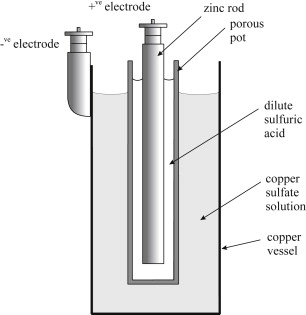
\includegraphics[width=0.7\linewidth]{Images/daniell}
            \caption{Daniell 전지}\label{f17}\cite{WINTERBONE2015497}
        \end{figure}
        \textbf{전해질 농도차 전지(Electrolyte concentration cell)}에서는 전해질의 농도를 제외하고 전극 칸의 구성이 동일하다. 한편 
        \textbf{전극 농도차 전지(Electrode concentration cell)}에서는 전극 그 자체가 서로 다른 농도를 가진다: 예를 들어, 서로 다른 압력으로 작동하는 
        기체 전극의 경우, 또는 아말감과 같이 동일한 물질로 이루어진 전극이지만 그 농도가 다른 경우이다. 
        \par Daniell 전지에서 두 전해질을 분리하는 다공성 용기와 같이, 서로 다른 두 전해질이 맞닿을 경우 생기는 전극 퍼텐셜을 \textbf{액간 전위(Liquid junction potential, $E_\mathrm{lj}$)}라 
        한다. 전해질 간 확산이 시작할 때, 두 이온의 이동도가 다르면 처음에는 더 큰 액간 전위가 형성된다. 
        이후 확산이 더 일어나면 특정 값으로 수렴하게 된다. 
        \par 염다리를 도입함으로써, 액간 전위를 1-2 mV 수준으로 줄일 수 있다. 염다리 내에 존재하는 이온의 
        이동도는 유사해야 한다. 이 경우 염다리 양쪽 끝의 액간 전위가 비슷해져, 서로 거의 상쇄된다.
        \par 전지는 다음과 같이 나타낸다:
        \begin{defn}[전지를 나타낼 때 쓰는 기호]
        \begin{enum}
            \item $\vert$ 상 또는 화학종 간 계면
            \item $\vdots$ 액간 계면
            \item $\vert \vert$ 액간 전위가 없다고 가정하는 계면
        \end{enum}
        \end{defn}
        따라서 Figure \ref{f17}의 전지는 다음과 같이 나타낼 수 있다:
        \begin{center}
            Zn(s) $\vert$ H$_2$SO$_4$(aq) $\vdots$ CuSO$_4$(aq) $\vert$ Cu(s)
        \end{center}
        \par 갈바니 전지에서는 자발적 화학 반응이 일어난다. 이때 \textbf{전지 반응(Cell reaction}은 
        오른쪽 전극이 환원 전극, 왼쪽 전극이 산화 전극일 때의 화학 반응이다. 이를 화학 반응식으로 나타내기 위해서는 오른쪽 전극의 반쪽 반응과 왼쪽 전극의 반쪽 반응을 환원 반응으로 나타낸 후에 왼쪽 전극의 반쪽 반응을 
        오른쪽 전극의 반쪽 반응에서 빼면 된다. 만약 전하 균형이 맞지 않을 경우 계수를 조정할 수 있다.
        \par 화학 평형에 도달하지 않은 전지 반응이 일어나는 전지에서는 외부 회로로 전자를 흘려보냄으로써 
        전기적 일을 할 수 있다. 주어진 양의 전자가 할 수 있는 일의 양은 전위차에 비례한다. 전체 반응이 평형에 
        도달하여 전위차가 발생하지 않은 전지는 할 수 있는 전기적 일이 없다.
        \par \ref{ch3sub4}에서 보인 것과 같이, $w_\mathrm{add,max} = \Delta G$에 해당한다. 전기화학에서는 추가적인 비팽창 일을 전기적 일($w_e$)로. 다루는 계는 전지로, 반응 Gibbs 에너지는 전지 반응의 Gibbs 에너지로 본다. 최대 일을 얻기 위해서는 반응이 가역적으로 일어나야 하므로, 여기에서는 
        반응이 가역적으로 일어난다고 본다. 또한 $\Delta_r G$는 $RT \ln Q$와 관련이 있으므로, 전지는 일정한 구성을 가지고 있다고 본다. 따라서 $\Delta_r G$를 구하기 위해서는 전지가 가역적으로, 일정한 구성으로 작동한다는 것을 가정해야 한다. 
        이때 전류는 흐르지 않는다. 이러한 가정을 통해 정의되는 전위차를 \textbf{전지 전위(Cell potential, $E_\mathrm{cell}$)}라 
        한다.
        \par 전지 전위는 다음과 같이 정의된다: 전지 반응이 $\difform \xi$만큼 일어났을 때, 식 \ref{rxngibbs}에 의해 
        \begin{equation*}
            \difform G = \Delta_r G \difform \xi
        \end{equation*}
        가 성립한다. 이때 $\difform G$는 최대 비팽창 미소 일에 해당하고, 이때 비팽창 일은 전기적 
        일에 해당한다:
        \begin{equation*}
            \difform w_e = \Delta_r G \difform \xi
        \end{equation*}
        이때 반응 1 mol 당 전자가 $\nu$ mol만큼 이동한다고 가정하자. $\difform \xi$만큼의 반응이 일어날 때 이동하는 전하량은 전자의 기본 전하량 $e$에 대해 $-\nu e N_\mathrm{A} \difform \xi$이다. 
        따라서 전기적 일 $\difform w = \phi \difform Q$에 대해, $\phi$는 전기 퍼텐셜에 해당하므로 $\phi = E_\mathrm{cell}$이다. 
        따라서 \textbf{Faraday 상수(Faraday's constant)} $F = e N_\mathrm{A}$로 정의하면, 
        다음이 성립한다:
        \begin{equation*}
            \difform w_e = -\nu F E_\mathrm{cell} \difform \xi
        \end{equation*}
        따라서 두 식에 의해, 다음이 성립한다:
        \begin{law}[전지 전위와 반응 Gibbs 에너지 사이의 관계]
        \begin{equation*}
            -\nu F E_\mathrm{cell} = \Delta_r G
        \end{equation*}
        \end{law}
        만약 전지 반응이 자발적이면(즉 $\Delta_r G < 0$이면), 전지 전위는 양수이다. 반대로, 만약 전지 반응의 반대 반응이 자발적이면(즉 $\Delta_r G > 0$이면), 전지 전위는 음수이다. 반응이 평형에 가까우면, 
        전지 전위는 매우 작다.
        \par 반응 Gibbs 에너지를 표준 반응 Gibbs 에너지와 비교한 식 $\Delta_r G = \Delta_r G^\circlehbar + RT\ln{Q}$에서, 양변을 $-\nu F$로 나누면 $E_\mathrm{cell} = \Delta_r G / \left(-\nu F\right)$에서
        \begin{equation*}
            E_\mathrm{cell}=-\frac{\Delta_r G^\circlehbar}{\nu F}-\frac{RT}{\nu f}\ln{Q}
        \end{equation*}
        이다. 이때 \textbf{표준 전지 전위(Standard cell potential, $E_\mathrm{cell}^\circlehbar$)}를 
        다음과 같이 정의한다:
        \begin{defn}[표준 전지 전위]
        \begin{equation*}
            E_\mathrm{cell}^\circlehbar = -\frac{\Delta_r G^\circlehbar}{\nu F}
        \end{equation*}
        \end{defn}
        따라서 다음이 성립한다:
        \begin{law}[Nernst 등식]
        \begin{equation*}
            E_\mathrm{cell} = E_\mathrm{cell}^\circlehbar - \frac{RT}{\nu F}\ln{Q}
        \end{equation*}
        \end{law}
        이 등식을 \textbf{Nernst 등식(Nernst equation)}이라 한다.
        \par $Q=K$일 때, $E_\mathrm{cell}=0$을 만족한다. 따라서 다음이 성립한다:
        \begin{law}[표준 전지 전위와 평형 상수 사이의 관계]
        \begin{equation*}
            E_\mathrm{cell}^\circlehbar = \frac{RT}{\nu F}\ln{K}
        \end{equation*}
        \end{law}
        이온의 표준 생성 Gibbs 에너지는 $\Delta_f G^\circlehbar\left(\text{H}^+\text{,aq}\right)=0$으로 정의한다. 이를 기준으로 반쪽 반응의 표준 환원 전위를 측정한다.
        \par 표준 전지 전위를 온도로 미분한 값은. $\displaystyle\left(\frac{\partial G}{\partial T}\right)_p = -S$에서 다음과 같이 유도된다:
        \begin{equation*}
            \frac{\difform E_\mathrm{cell}^\circlehbar}{\difform T}=\frac{\Delta_r S^\circlehbar}{\nu F}
        \end{equation*}
        이때 편미분이 아닌 이유는, 전지 반응은 압력에 무관하기 때문이다. 한편, 전지 반응의 반응 엔탈피를 구하는 방법은 다음과 같다:
        \begin{obs}[전지 반응의 반응 엔탈피]
        \begin{equation*}
            \begin{aligned}
                \Delta_r H^\circlehbar &=\Delta_r G^\circlehbar + T \Delta_r S^\circlehbar\\
                &= -\nu F\left(E_\mathrm{cell}^\circlehbar-T\frac{\difform E_\mathrm{cell}^\circlehbar}{\difform T}\right)
            \end{aligned}
        \end{equation*}
        \end{obs}
        따라서 전기화학적인 방법으로 전지 반응의 반응 엔탈피를 구할 수 있다.
        \section{전극 전위}
        \hspace{\parindent} 다음 전극을 \textbf{표준 수소 전극(Standard hydrogen electrode, SHE)}이라 하고, 이 전극의 표준 전극 전위를 모든 온도에서 $E^\circlehbar=0$으로 정의한다:
        \begin{defn}[표준 수소 전극]
        \begin{center}
            Pt(s) $\vert$ H$_2$(g) $\vert$ H$^+$(aq)
        \end{center}
        \end{defn}
        이때 수소 기체의 퓨가시티 $f_{\mathrm{H}_2} = 1$, 수소 이온의 활동도 $a_{\mathrm{H}^{+}}=1$이어야 한다. 
        산화-환원 쌍 X의 \textbf{표준 전위(Standard potential, $E^\circlehbar\left(X\right)$)}은 
        표준 수소 전극을 산화극으로 하는 다음과 같은 화학 전지의 표준 전지 전위로 정의한다:
        \begin{defn}[표준 전위]
        \begin{center}
            Pt(s) | H$_2$(g) | H$^{+}$(aq) || X, $E^\circlehbar\left(X\right)=E^\circlehbar_\mathrm{cell}$
        \end{center}
        \end{defn}
        표준 전지 전위는 두 전극의 표준 전위 차로 계산할 수 있다:
        \begin{obs}[표준 전지 전위]
        \begin{center}
            L $\vert \vert$ R, $E^\circlehbar_\mathrm{cell}=E^\circlehbar\left(R\right) - E^\circlehbar\left(L\right)$
        \end{center}
        \end{obs}
        \par 표준 전위를 구하는 방법을 Ag/AgCl 전극을 통해 알아보자. 다음과 같은 전지를 통해 측정한다:
        \begin{center}
            Pt(s) | H$_2$(g) | HCl (aq, $b$) | AgCl(s) | Ag(s)
        \end{center}
        이때 전체 반응은 다음과 같이 진행된다:
        \begin{center}
            $\displaystyle\frac{1}{2}$ H$_2$(g) + AgCl(s) $\rightarrow$ HCl(aq) + Ag(s)
        \end{center}
        따라서 표준 전지 전위는 다음과 같다:
        \begin{equation*}
            E^\circlehbar_\mathrm{cell}=E^\circlehbar\left(\text{AgCl/Ag,Cl}^{-}\right)-E^\circlehbar\left(\text{SHE}\right)=E^\circlehbar\left(\text{AgCl/Ag,Cl}^{-}\right),\, \nu=1
        \end{equation*}
        따라서 Nernst 등식은 다음과 같이 쓸 수 있다:
        \begin{equation*}
            E_\mathrm{cell}=E^\circlehbar\left(\text{AgCl/Ag,Cl}^{-}\right)-\frac{RT}{F}\ln{\frac{a_{\mathrm{H^+}}a_{\mathrm{Cl^-}}}{a_\mathrm{H_2}^{1/2}}}
        \end{equation*}
        만약 표준 상태라면, $a_\mathrm{H_2}=1$를 만족한다. 또한, $a_\mathrm{H^+}=\gamma_\pm b/b^\circlehbar$이고 
        $a_\mathrm{Cl^-}=\gamma_\pm b/b^\circlehbar$이므로 다음과 같이 쓸 수 있다:
        \begin{equation*}
            E_\mathrm{cell}=E^\circlehbar-\frac{RT}{F}\ln{\frac{{\gamma_\pm}^2 b^2}{{b^\circlehbar}^2}}
        \end{equation*}
        \begin{obs}\label{eqn268}
        \begin{equation*}
            E_\text{cell}+\frac{2RT}{F}\ln{\frac{b}{b^\circlehbar}}=E^\circlehbar-\frac{2RT}{F}\ln{\gamma_\pm}
        \end{equation*}
        \end{obs}
        이때, Debye-Hückel 한계 법칙에 의해 $b\rightarrow 0$일 때
        \begin{equation*}
            \log{\gamma_\pm}=-A\left\vert z_+ z_-\right\vert I^{1/2}=-A\left(b/b^\circlehbar\right)^{1/2}
        \end{equation*}
        가 성립하고, 따라서 식 \ref{eqn268}를 다시 정리하면
        \begin{equation*}
            E_\text{cell}+\frac{2RT}{F}\ln{\frac{b}{b^\circlehbar}}=E^\circlehbar\frac{2ART\ln{10}}{F}\left(\frac{b}{b^\circlehbar}\right)^{1/2}
        \end{equation*}
        이다. 이때 $\displaystyle C=\frac{2ART\ln{10}}{F}$로 두면 다음이 성립한다:
        \begin{equation*}
            E_\text{cell}+\frac{2RT}{F}\ln{\frac{b}{b^\circlehbar}}=E^\circlehbar + C\times\left(\frac{b}{b^\circlehbar}\right)^{1/2}
        \end{equation*}
        따라서 $\left(b/b^\circlehbar\right)^{1/2}$를 $x$축으로 하고 $E_\text{cell}+\frac{2RT}{F}\ln{\left(b/b^\circlehbar\right)}$을 $y$축으로 하여 선형회귀하면 $y$절편이 표준 전위에 해당하게 된다.
        \par 관여하는 전자 수가 다른 두 반쪽 반응을 결합하기 위해서는 다음과 같은 식을 이용한다:
        \begin{equation*}
            \nu_c E^\circlehbar\left(c\right)=\nu_a E^\circlehbar\left(a\right) - \nu_b E^\circlehbar\left(b\right)
        \end{equation*}
        이때 $\nu_r$은 각각의 반쪽 반응에서 관여하는 전자의 수이다.
        \par 화학 전지 L $\vert\vert$ R (즉 Ox$_L$/Red$_L$ $\vert\vert$ Ox$_R$/Red$_R$)이 있을 때, 다음 반쪽 반응과 표준 전지 전위를 관례적으로 이용한다:
        \begin{center}
            Ox$_R$ + $\nu$e$^- \rightarrow$ Red$_R$, Ox$_L$ + $\nu$e$^- \rightarrow$ Red$_L$
        \end{center}
        \begin{equation*}
            E_\text{cell}^\circlehbar = E^\circlehbar\left(R\right)-E^\circlehbar\left(L\right)
        \end{equation*}
        이때 전체 반응은 다음을 관례적으로 이용한다:
        \begin{center}
            R $-$ L : Red$_L+$ Ox$_R \rightarrow$ Ox$_L+$ Red$_R$
        \end{center}
        만약 이 반응의 $K>1$이면 $E_\text{cell}^\circlehbar$이고, $E^\circlehbar\left(R\right)>E^\circlehbar\left(L\right)$이다. 이 경우 Red$_L$이 Ox$_R$을 환원시키는 경향이 더 크다. 즉, 
        \textbf{$E^\circlehbar\left(R\right)>E^\circlehbar\left(L\right)$일 때 환원시키는 (즉 자신이 산화되는) 경향은 Red$_L$이 Red$_R$보다 더 크다.}
        \textbf{전위 서열(Electrochemical series)}은 금속 원소가 산화되는 경향성을 표준 전위를 기준으로 
        늘어 놓은 열이다.\footnote[17]{우리가 "칼카나마알아철니..."로 외우는 그 목록이 맞다.} 표준 전위가 낮을수록 금속 원소가 산화되는 (즉 다른 화학종을 환원시키는) 경향이 강하므로, 목록의 아래에 있을수록 환원제로 작용하는 경향성이 강하다.
        \par 마지막으로, Nernst 식을 이용하여 활동도 계수 및 평형 상수를 결정할 수 있다.

\backmatter
\pagestyle{plain}

\renewcommand{\bibname}{참고문헌}

\bibliographystyle{ieeetr}
\bibliography{ref}
\addcontentsline{toc}{chapter}{참고문헌}

\end{document}